\documentclass[a4paper,12pt, twoside]{memoir}   	% use "amsart" instead of "article" for AMSLaTeX format

\pagestyle{ruled} %ruled, companion, headings
%also: empty, plain, headings, myheadings, simple, ruled, Ruled,
%also: companion, book, chapter, cleared, part, title, titlepage
\chapterstyle{madsen} % madsen
%also: default, section, hangnum, companion, article, reparticle
%also: bianchi, brighthurst, brotherton, chappell, crosshead, culver,
%also: dash, demo2, demo3,  dowdingell, ell, ger, komalke, lyhne, madsen
%also: ntglike, pederson,  southall, book, thatcher, veelo, verville,
%also: wilsondob


%% \usepackage[switch, modulo]{lineno}
%% \linenumbers


\usepackage{geometry}                		% See geometry.pdf to learn the layout options. There are lots.
%% \geometry{letterpaper}                   		% ... or a4paper or a5paper or ...
\geometry{vmargin=3cm}%% hmargin=2cm
\usepackage{graphicx}
\usepackage{color}
\usepackage[dvipsnames]{xcolor}
\usepackage{enumerate}
\usepackage{amssymb}
\usepackage{footnote}
\usepackage{enumerate}
\usepackage{eucal}
\usepackage{amsmath}
\usepackage{braket}
\usepackage[utf8]{inputenc}
\usepackage[english]{babel}
\usepackage{hyperref}
\usepackage{xspace}
\usepackage{pdfpages}
\usepackage{subcaption}
\usepackage[margin=2cm]{caption}
%% pour empêcher la cesure des mots
\pretolerance=10000
\tolerance=1000
\emergencystretch=10pt

\captionsetup[figure]{font=footnotesize}
\captionsetup[subfigure]{font=footnotesize}
\captionsetup[table]{font=footnotesize}
\captionsetup[subtable]{font=footnotesize}
\captionsetup[tabular]{font=footnotesize}

\hypersetup{
  colorlinks,
  citecolor=red,
  filecolor=red,
  linkcolor=red,
  urlcolor=red
}

\setcounter{tocdepth}{2}
\setcounter{secnumdepth}{3}

\newcommand{\zeronu}{0\nu\beta\beta}
\newcommand{\twonu}{2\nu\beta\beta}
\newcommand{\Se}{$^{82}$Se}
\newcommand{\Nd}{$^{150}$Nd}
\newcommand{\Mo}{$^{100}$Mo}
\newcommand{\U}{$^{238}$U}
\newcommand{\Th}{$^{232}$Th}
\newcommand{\K}{$^{40}$K}
\newcommand{\Tl}{$^{208}$Tl}
\newcommand{\Co}{$^{60}$Co}
\newcommand{\Pb}{$^{208}$Pb}
\newcommand{\Bi}{$^{214}$Bi}
\newcommand{\Rn}{$^{222}$Rn}
\newcommand{\Qbb}{Q_{\beta\beta}}
\newcommand{\Bckunit}{\text{counts.keV}^{-1}\text{.kg}^{-1}\text{.y}^{-1}}
\newcommand{\Tbeta}{T_{1/2}^{0\nu}}
\newcommand{\Ttwonu}{T_{1/2}^{2\nu}}
\newcommand{\mbb}{m_{\beta\beta}}
\newcommand{\Pint}{P$_{int}$}

\newcommand\myshade{85}
\colorlet{mylinkcolor}{violet}
\colorlet{mycitecolor}{YellowOrange}
\colorlet{myurlcolor}{Aquamarine}
\usepackage{hyperref} %backref
\hypersetup{
  linkcolor  = mylinkcolor!\myshade!black,
  citecolor  = mycitecolor!\myshade!black,
  urlcolor   = myurlcolor!\myshade!black,
  colorlinks = true,
}

\newenvironment{itemize*}%
               {\begin{itemize}%
                   \setlength{\itemsep}{0pt}%
                   %\setlength{\parskip}{0pt}
               }%
               {\end{itemize}}


               %\title{}

               \includeonly{Sensitivity/Sensitivity}
               %% \includeonly{commissioning/commissioning}
               %% \includeonly{timedifference/timedifference}
               %% \includeonly{SNdemonstrator/SNdemonstrator}

               \begin{document}
               %\maketitle
               \includepdf{1couverture}
               \cleardoublepage
               \tableofcontents

               \chapter*{Introduction}
\label{ch:intro}
\addcontentsline{toc}{chapter}{Introduction}

It is always interesting to take a historical approach when talking about a scientific discovery. This allows us to put into perspective knowledge that is now considered to have been acquired.

The Standard Model of Elementary Particle Physics attempts to describe the world around us on scales that were inconceivable two centuries ago.
A little over a hundred years ago, Henri Becquerel discovered what we today call radioactivity, with the observation of $\beta$ decay.
This historical discovery was nevertheless accompanied by profound questioning, since the $\beta$ particle emitted during this decay, which turned out to be an electron, only carries away part of the available energy for the reaction.
This observation was contrary to the first principle of thermodynamics on the energy conservation, and some scientists postulated that this fundamental law was being violated.
It took 35 years for an eminent scientist by the name of Wolfgang Pauli to propose the existence of the \emph{neutrino} ($\nu$) - for small neutron in Italian - as a solution to the problem of missing energy.
Three years later Enrico Fermi laid the foundations for the first mathematical formulation of what is today the Lagrangian of weak interaction.
It was another 25 years, 60 years after the discovery of $\beta$ radioactivity, before the neutrino was experimentally observed by Clyde Cowan and Frederick Reines.
The neutrino adventure had only just begun.

Why is this particle, although abundantly produced in the sun in the atmosphere and in the earth, so difficult to detect?
It is because it interacts very little with the matter - electrons and quarks - that constitutes us, being sensitive only to the weak interaction (of short range), and to the gravitational force (very weakly since the mass of the neutrino is extremely low, so much that it was believed massless for a long time).

In the current model of particle physics, neutrinos are actually described as massless.
It was Bruno Pontecorvo who proposed in 1957 that neutrinos could oscillate between their different mass states, based on the already known model of oscillation of neutral kaons.
To be valid, this model then presupposed that neutrinos had a non-zero mass.
It was the SuperKamiokande experiment that first observed this phenomenon in 1998, demonstrating that at least two of the three neutrino flavours have a non-zero mass.
The Standard Model of particle physics is then no longer sufficient to account for this particle properties, opening the way to physics beyond the Standard Model.

It now remains to be discovered how this particle acquires its mass.
Indeed, having a neutral charge under the three fundamental interactions described by the Standard Model, two mass generation mechanisms are foreseeable.
The first is to assume that, like all other fermions, the neutrino obtains its mass through the Higgs mechanism, leading irremediably to the assumption of the existence of a sterile neutrino.
The second, proposed by Ettore Majorana, assumes that the neutrino is its own antiparticle, giving the neutrino its mass with the addition in the Lagrangian of the Majorana mass term.
If this assertion is the one that applies to neutrinos, then a disintegration, prohibited in the Standard Model, is possible.
It is called \emph{neutrinoless double beta decay} ($\zeronu$), to contrast with the \emph{two neutrinos double beta decay} ($\twonu$) allowed by the Standard Model and already observed for several isotopes.
In the former disintegration, two simple $\beta$ decays take place simultaneously in the same nucleus, in which the two neutrinos are absorbed, allowing the total energy of the reaction to be distributed between the two exiting electrons.
For reasons that are detailed in the first chapter of this manuscript, which deals with the phenomenology of the neutrino, this disintegration is only possible if the neutrino is a Majorana particle.

Several experiments, also described in the first chapter, are dedicated to the search for this disintegration which, if it exists, is expected to be extremely rare.
%%Its observation would prove the neutrino is a Majorana particle.
The SuperNEMO experiment, on which I conducted my PhD, is one of them.
Successor of the NEMO experiments, it uses a unique combination of technologies, described in detail in the second chapter, allowing to trace the path of the electrons resulting from double $\beta$ disintegrations -with a wire chamber-, and also to measure their energies - with a segmented electromagnetic calorimeter.

These generation of experiments differ from one another in the technology they use, and also in the sensitivity they can achieve in the search for this decay.
Within the framework of this PhD, I carried out a sensitivity study of this experiment presented in the third chapter, determining the influence that several characteristics of the detector can have on it.

All these experiments are designed to observe, should this process exist, an extremely rare physical event.
They are thus constrained to focus on the background which may disturb the measurement and have a non-negligible impact on their sensitivity to this disintegration.
In this perspective, the fourth chapter presents a new technique to identify the events resulting from one of the main background for this experiment, which is the natural disintegration of an isotope from the uranium 238 decay chain, found in the detector's components.
To effectively reject this background, I also study the impact on the sensitivity of the accuracy with which we measure the arrival time of particles in the calorimeter.
To complete this theoretical analysis based on simulations of the detector, the fifth chapter gives an overview of the data taken at Modane with the SuperNEMO calorimeter and of the analysis aiming to characterise the time resolution for a large part of the optical modules.

When I joined the LAL team at Orsay (now IJCLab) as a PhD student, SuperNEMO was already largely built in the Modane underground laboratory.
I had the opportunity to actively participate in the completion of its assembly, as well as in the analyses of the first commissioning data described in the last chapter, thus completing the experimental knowledge acquired during this PhD.

               \chapter{Phenomenology of particle physics}
\section{The Standard Model of particle physics}
\subsection{Bosons}
\subsection{Fermions}
\subsection{$\twonu$ decay}
\subsection{Where the Standard Model ends}
\section{Going beyond the Standard Model with neutrinos}
\subsection{Neutrino flavors and oscillations}
\subsection{Neutrino masses and nature}
\label{subsec:nu_mass_nature}
\subsection{Other searches beyond the Standard Model with neutrinos}

               \chapter{The SuperNemo demonstrator}
\label{ch:detector}

\section{The SuperNemo demonstrator}
\subsection{Comparison with Nemo$3$ experiment}
\subsection{Expermimental design}
\subsection{Sources}
\subsection{Tracker}
\subsection{Calorimeter}
\label{subsec:SN_calo}



\subsubsection{Scintillator}





\subsubsection{Photomultiplier}
\label{sec:calorimeter}
\subsection{Calibration systems}
\subsection{Control Monitoring system}
\subsection{Electronics}

\section{The backgroung of SuperNEMO}
\label{sec:SNbkg}
\subsection{Internal background}
\label{subsec:SNbkg_internal}

Trace quantities of naturally-occurring radioactive isotopes can occasionally produce two-electron events and thus can mimic $\beta\beta$-decay events.
The largest contributions come from isotopes of decay chains of $^{238}$U, $^{232}$Th and $^{40}$K, which disintegration occur inside the source foils, as well as inside the tracking volume.

Décire la contamination mesurée des sources, et du radon dans la partie suivante

\subsection{External background}
Radon:\\
Radon is a noble gas which occurs as an indirect decay product of uranium and thorium.
Due to its chemical properties, radon has a long diffusion length in solids, making it difficult to remove.
Radon contaminations inside the tracker volume is a major background to the rare event experiments such as SuperNEMO.
Simulations show that, to achieve the designed sensitivity, the level of radon must not exceed $0.15$ mBq/m$^{3}$ since its decay daughter \Bi, $\Qbb= 3.2$ MeV can mimic a $\zeronu$ event.
Radon concentration measurements inside the demonstrator tracker have been performed by the SuperNEMO collaboration, revealing an activity of $0.15\pm0.02$ mBq/m$^{3}$, through the combination of an anti-radon tent and an air-flushing method.

%%Repris d'un article -> a changer:
They are outgased in the air from the rock walls of the experimental hall and can enter the detector either through tiny gaps between sectors or through gas pipe joints.
The progeny of radon and thoron produces $\gamma$-rays and $\beta$ decays accompanied by internal conversion (IC), Møller or Compton scattering.
\subsection{Background specifications}
\subsection{Measured demonstrator background levels}

\section{Magnetic field}
\label{sec:magnetic_field}

\section{The SuperNemo software}
\label{sec:SNsoftware}
\subsection{Simulation}

As described in Sec.~\ref{sec:SNsoftware} of Chapter~\ref{ch:detector}, the SuperNEMO collaboration developed its own simulation, reconstruction and analysis environment.
The Falaise software, specifically designed by and for the SuperNEMO collaboration, holds the \verb!C++! library for the event reconstruction and analysis of simulated and real data.
Especially, it contains the geometry, the detector material, the event data model, the reconstruction algorithms and the data analysis.
Finally, the SNFee software is a tool package for the configuration, control and monitoring of the SuperNEMO front-end electronics.

\subsection{Reconstruction}

               \chapter{Sensitivity of the SuperNEMO demonstrator to the $\zeronu$}
\label{ch:sensitivity}

In this chapter, we present a study aiming to evaluate the SuperNEMO's sensitivity to the $\zeronu$ decay, and the corresponding effective neutrino mass.
Studies of this kind have already been conducted, and the final detector is expected to exclude half-lives up to $1.2\times 10^{26}$ y ($90\%$ CL), with an exposure of $500$ kg.y for the \Se\footnote{Supposing Selenium-$82$ $\zeronu$ decays through the exchange of a light Majorana neutrino.}~\cite{art:SuperNEMO2010}.
In $2015$ began the demonstrator installation at the Laboratoire Souterrain de Modane, aiming to assess the feasibility of such a large scale detector based on the NEMO-$3$ technology.
With an exposure of $17.5$ kg.y, the demonstrator could reach a sensitivity on the $\zeronu$ process of $5.3\times 10^{24}$ y ($90\%$ CL) \cite{CalvezThesis}.

At the time of the current analysis, the coil, which is supposed to deliver a magnetic field inside the detector, was not yet installed on the demonstrator.
We aim to explore the impact, on both the demonstrator and final detector sensitivity, of the presence of this magnetic field.
The findings of this study will participate in the final decision on the installation of the coil.
In a context of investigating the demonstrator and final detector's capabilities, different internal source contamination levels are considered.
The topology of interest is the two electrons ($2e$) topology, and we use the total energy sum to discriminate the signal from the background events.
Thanks to SuperNEMO tracking capabilities, topological informations are also exploited to improve the sensitivity.

\begin{itemize}
\item parler des autres isotopes qu''on voudrait mettre
\end{itemize}

%%The sensitivity is given as an upper limit, in case we do not observe the expected signal.


\section{The $\zeronu$ Signal and background model}
\label{sec:sensitivity_simus}

A full simulation for the demonstrator was performed, in order to determine the upper limit on $\zeronu$ half-life that can be probed with SuperNEMO.
This sensitivity greatly depends on the number of background events detected but non-rejected during the data taking.
The expected number of events for natural isotopes depend on their activities inside the source foils (for Thallium-$208$ and Bismuth-$214$), or on the tracker's wires (for Radon-$222$ decaying in Bismuth-$214$).
It was necessary, during the design of the detector, to constrain their maximal tolerable activities, to guarantee a high sensitivity to the $\zeronu$ disintegration~\cite{internal:SNphysicsCase}.
These values are given in the table, per disintegration unit per second, for one kg of source material, or for one m$^{3}$ of gas inside the tracker.

Meanwhile, the amount of expected $\twonu$ decays is mainly driven by its $\Ttwonu$ value: the higher the half-life of this process, the lower its contribution in the total number of expected background.
For Selenium-$82$ sources, we take the $\twonu$ half-life measured by NEMO-$3$, $\Ttwonu = 9.39 \pm 0.17$ (stat) $\pm 0.58$ (syst) $\times 10^{19}$ years~\cite{art:NEMO2018}.

%%
In the Tab.~\ref{tab:sensitivity_simulations} is summarised the expected number of signal and background events, both for the SuperNEMO demonstrator and final detector.
We also present, for each of the process, the amount of simulated events.
\begin{table}[h]
  \centering
  \begin{tabular}{|l|cc|c|}
    \hline
    Type of decay &\multicolumn{2}{c|}{Expected decays} & Simulated decays \\
    & Demonstrator & Final detector & \\
    \hline\hline
    $\zeronu$ ($\Tbeta = 2.5\,10^{23}$ y) & $3.6\,10^{2}$ & $1.0\,10^{4}$ & $1.0\,10^{7}$ \\
    $\twonu$ ($\Ttwonu = 9.39\times 10^{19}$ y) & $9.5\,10^{5}$ & $2.7\,10^{7}$ & $1.0\,10^{7}$ \\
    \Tl\ ($\mathcal{A}^{\text{Tl}} = 10\,\mu$Bq/kg)  & $5.5\,10^{3}$ & $1.6\,10^{5}$ & $1.0\,10^{7}$ \\
    \Bi\ ($\mathcal{A}^{\text{Bi}} = 2\,\mu$Bq/kg) & $1.1\,10^{3}$ & $3.1\,10^{4}$ & $1.0\,10^{7}$ \\
    \Rn\ ($\mathcal{A}^{\text{Rn}} = 0.15$ mBq/m$^{3}$) & $1.8\,10^{5}$ & $7.2\,10^{6}$ & $1.0\,10^{8}$ \\
    \hline
  \end{tabular}
  \caption{Expected and simulated decays for different processes, both for the demonstrator ($17.5$ kg.y) and for the final detector exposures ($500$ kg.y), assuming target background activities are reached: $\mathcal{A}^{\text{Tl}}~=~10\,\mu$Bq/kg, $\mathcal{A}^{\text{Bi}}~=~2\,\mu$Bq/kg, $\mathcal{A}^{\text{Rn}}~=~0.15$ mBq/m$^{3}$.
    The measured half-life $\Ttwonu~=~9.39\times~10^{19}$ y for Selenium-$82$'s $\twonu$ is taken, and we assume $\Tbeta = 2.5\times 10^{23}$ y~\cite{art:NEMO2018}.
    \label{tab:sensitivity_simulations}}
\end{table}
%The value entered for the $\Tbeta$ is given only illustratively: the decay has never been observed, so we choose the limit on the half-life obtained with NEMO-$3$~\cite{art:NEMO2018}.
The figures in the central column represent the total number of disintegrations, without taking into account any technique to reject background, and for the total energy window.


%%

%%


Nevertheless, the number of decays presented in the table are expected to be extremely reduced, notably by the application of event selections aimed at maximising the sensitivity to the excluded $\zeronu$ half-life (Sec.~\ref{sec:sensitivity_ev_selection}).
Moreover, this effect is augmented by the fact that, for the current sensitivity analysis, we will focus on a narrow energy window, called \emph{region of interest}, whose usefulness will be described in more detail in Sec.~\ref{sec:Nbkg_ROI}.
Therefore, to properly conduct this sensitivity study, it was necessary to simulate a large number of events, so that the signal and backgrounds are correctly represented in the region of interest.
Let us now detail the simulations produced as part of this analysis.

%% c'est pas plutôt à cause du fait que tous les decays de ces isotopes ne sont pas intéressants ?
%% du coup dans la topologie 2e il ne reste plus rien

\subsection{The $\zeronu$ signal}

The SuperNEMO detector was designed to search for the never-observed $\zeronu$ decay.
In the following, we assume the underlying mechanism for this decay is the exchange of a light Majorana neutrino, the so-called mass mechanism (MM), as it is the most widespread mechanism.
The hypothetical $\zeronu$ signal would be detected as an excess of events in the region of interest, with respect to the predicted background contamination level.
Some $10^{7}$ $\zeronu$ events were simulated inside the source foils, using the DECAY$0$ software~\cite{art:decay0}.
The simulations are normalised assuming the half-life excluded by NEMO-$3$, $\Tbeta = 2.5\,10^{23}$ y ($90\%$~CL)~\cite{art:NEMO2018}.

\subsection{Inside detector backgrounds}

In addition with the $\zeronu$ decay, we simulated different types of backgrounds, that could mimic the searched signal.

\subsubsection{Internal backgrounds}

The so-called \emph{internal backgrounds} stand for decays occurring inside the source foils, presenting the same signature as the $\zeronu$ signal.
These backgrounds, already introduced earlier, are the $\twonu$ of the source isotope, as well as disintegrations of \Tl\ and \Bi.


\subsubsection*{The $\twonu$ process}

In the full energy range, the allowed $\twonu$ decay stands as the dominant internal background type.
Its total energy spectrum is a continuum, whose ending point should stands at $\Qbb = 2.99$ MeV, but is slightly increased by the detector's energy resolution.
We simulated $10^{7}$ events of this decay inside the source foils, in the full energy window.
However, above a certain energy value, the number of $\twonu$ events decreases very quickly.
To offset this effect, we simulated additional $10^{7}$ of this decay on a slightly lower energy range, that is to say above $2$ MeV.
The second set of simulations is normalised with the first one.
In this way, the lack of $\twonu$ simulated events in the high-energy tail is avoided, without requiring too high computational resources.

\subsubsection*{Source foils contamination by natural isotopes}

As described in Sec.~\ref{subsec:SNbkg_internal}, after sources purification, remaining natural isotopes such as \Tl\ or \Bi\ can still be present inside the foils.
This class of contamination constitutes the principal internal source of background, with the $\twonu$ decay.
We simulated $10^{7}$ decays both for the two isotopes, inside the source foils.

\subsubsection{Tracker contamination by natural isotopes}

The presence of gaseous Radon-$222$ inside the tracker, mainly deposited on the copper wires, can produce events similar to internal one.
In fact, one of the progeny of Radon-$222$, the Bismuth-$214$, can decay on (or near) a foil, and appear with a $2e$ topology, becoming hard to distinguish from a double beta decay candidate.
As this isotope is distributed throughout the whole tracking detection volume, to study the experiment's sensitivity, we simulated a large quantity of this decay on the tracker wires.
This way, we maximise the amount of \Bi\ events, coming from \Rn\ decays, in the region of interest.


\subsection{Outside detector backgrounds}

This background category is populated by the external $\gamma$-ray flux produced by radioactive isotope decays in detector components or surrounding laboratory rocks, as well as neutron interactions in the shield.
The most notorious difference is the fact that the SuperNEMO scintillator blocks are thicker than those of NEMO-$3$.
Therefore, a gamma is more likely to be detected and therefore, in that case, the event would not contribute to the background in the $2e$ channel.
As a consequence, for the same PMTs radioactivity, the external gamma background rate is expected to be less important for the SuperNEMO demonstrator than for NEMO-$3$.
Moreover, radiopurity measurements of SuperNEMO PMTs allow to conclude that their total activity is better than for those of NEMO-$3$, for the two principal considered isotopes \Tl\ and \Bi ~\cite{docdb:perrot2017}.
The NEMO-$3$ experiment set a limit on the external background number of counts, of $<0.2$ events in the $2e$ topology, for the energy range [$2.8$;$3.2$] MeV (two electrons energy sum), for an exposure of $34.3$ kg·y, with $^{100}$Mo sources~\cite{art:NEMO2015}.
Given the fact that SuperNEMO is expected to be better than NEMO-$3$ at rejecting external background events, we consider that all external backgrounds from outside the foil, apart from \Rn\ in the tracking volume, are expected to be negligible, and were not simulated.
Even if the regions of interest are slightly different between these two experiments, it produces negligible increase on the external background contribution.
 % Nevertheless, it is important to note that the energy window for SuperNEMO starts at $2.7$ MeV, and not at $2.8$ MeV as for NEMO-$3$, which could increase the external background contribution.\\

In the following we present an optimisation of the event selection that has been set up to maximise the excluded $\zeronu$ half-life in this specific topology.

%% \begin{itemize}
%% \item Justifier bdf externe avec article nemo3 (plus diff roi et meilleure eff)
%% \item The dominant two neutrino $\twonu$ background and the background due to foil contaminations were normalised assuming a demonstrator exposure of $17.5$ kg.y.
%% \item The total energy brought by the two electrons is a continuum presenting a reduced number of events in the region of interest, due to electron energy losses before reaching the calorimeter (mainly inside the dense source material, as well as inside the wire chamber).
%% \end{itemize}


\section{Event selection}
\label{sec:sensitivity_ev_selection}

For SuperNEMO, the $\zeronu$ signature is two-electrons events, emitted simultaneously from the same vertex on the source foils, with an energy sum compatible with $\Qbb = 2.99$ MeV for the Selenium-$82$.
Therefore, we conducted this analysis selecting only events matching the $2e$ topology, where a reconstructed particle is tagged as an electron if it has
\begin{itemize}
\item a vertex on the source foils,
\item a reconstructed track inside the wire chamber,
\item an associated calorimeter hit,
\item and a final criterion depending on the case under consideration.
  In fact, in the following, we will consider two separate cases.
  One where the magnetic field has a value of 25 Gauss along the z (vertical) axis of the detector, and one where the field is zero.
  In the first case, particles such as electrons and positrons of a few MeV will have a curved trajectory in the tracker.
  In the second case, the tracks of the particles will be straight lines.
  It is then necessary to adapt the selection of events to each case. When the magnetic field is switched on, we will then consider an additional criterion: a particle will be identified as an electron if its trace has a negative curvature.
\end{itemize}
All these selections represent the so-called \emph{first-order cuts}.

We present the total energy spectra for each simulated process, after event selection, in Fig.~\ref{fig:energy_spectra}.
\begin{figure}[h]
\centering
\begin{subfigure}[t]{0.7\textwidth}
  \centering
  \includegraphics[width=1.1\textwidth]{Sensitivity/fig_sensitivity/energy_spectrum_with_B_82Se.pdf}
  \captionsetup{justification=centering}
  \caption{
    \label{subfig:energy_spectra_full}}
\end{subfigure}
\hfill
\begin{subfigure}[t]{0.7\textwidth}
  \centering
  \includegraphics[width=1.1\textwidth]{Sensitivity/fig_sensitivity/energy_spectrum_with_B_82Se_zoom.pdf}
  \captionsetup{justification=centering}
  \caption{
    \label{subfig:energy_spectra_zoom}}
\end{subfigure}
\caption{Total energy spectra for the $\zeronu$ signal and main backgrounds, for (a) the full energy range, and (b) for the [$2.7$;$3.15$]~MeV energy range, whose optimisation is discussed in Sec.~\ref{sec:Nbkg_ROI}.
  \label{fig:energy_spectra}}
\end{figure}
% The total number of events for each decay represent the amount of selected $2e$ topologies.
The $\zeronu$ spectrum is peaked around $2.8$ MeV, as the available energy $\Qbb = 2.99$ MeV is degraded by electron energy losses before reaching the calorimeter (mainly inside the dense source material, as well as inside the wire chamber), explaining the asymmetric energy distribution.
% The progeny of \Rn\ produces $\gamma$-rays and $\beta$ decays accompanied by internal conversion (IC), Møller or Compton scattering, the dominant mechanism being the first one.
Whatever their origin, either Radon-$222$ contaminations inside the tracker gas, or internal contaminations of the source foils, the Bismuth-$214$ energy distributions have nearly the same shape.
Moreover, a great part of Radon-$222$ events have been rejected by the topological cuts.
Therefore, given the activities of \Rn\ in the tracker and \Bi\ inside the source foils, theses two background types both contribute at the same level in the full energy range.
The \Tl\ energy distribution reveals the internal conversion of the $2.614$ MeV gamma, emitted after \Tl\ $\beta^{-}$ disintegrations.

In what follows, we explain the steps that allowed to give a $\Tbeta$ sensitivity for the demonstrator.

\begin{itemize}
\item dire aussi que là on présente pour Se avec champ. Du coup ya la coupure du premier ordre sur la courbure de la trace aussi.
\end{itemize}



\section{Demonstrator sensitivity to the Selenium-$82$ $\zeronu$ decay}
\label{sec:Nbkg_ROI}

The two-electrons energy sum for the $\zeronu$ is expected as a peak at the end point of the $\twonu$ energy distribution.
This energy peak would be degraded by electron energy losses inside the source foils and wire chamber, as well as by the calorimeter energy resolution.
In Fig.~\ref{fig:energy_spectra} is represented, for specific data taking conditions, the energy spectra of the $\zeronu$ decay, assuming $\Tbeta = 2.5\times~10^{23}$~years.
The enlarged peak we are discussing is clearly noticeable around $2.7$~MeV. %in the [$2.7$;$3.15$]~MeV interval.
A widespread technique consists in constraining the $\zeronu$ decay searches to a narrow energy range, the so-called \emph{region of interest} (ROI), materialised by the two vertical dashed lines.
In the following, we expose general principles leading to determination of the best limit on $\Tbeta$, in the appropriate region of interest.
The reasoning presented is valid for all cases (all exposures, internal contamination levels and field conditions).
Nevertheless, we illustrate the method by presenting the results for the specific case were of the demonstrator (Selenium-$82$ sources, $17.5$ kg/y exposure), with the specified internal contamination levels ($\mathcal{A}^{\text{Tl}} = 10\,\mu$Bq/kg and $\mathcal{A}^{\text{Bi}} = 2\,\mu$Bq/kg).
%The optimisation of this energy window consists of cutting the full energy range in several sub-ranges, and compute the selection efficiencies for all energy sub-ranges.

In case of the non-observation of a $\zeronu$ signal, the expected upper limit on the half-life is provided for a given [$E_{\text{min}}$;$E_{\text{max}}$] energy range, and depends on the characteristics of the detector.
First, it depends on the signal detection efficiency $\epsilon_{0\nu}$ in this energy window, secondly on the source isotope nature, as well as the detector's exposure $m\times t$.
It follows
\begin{equation}
  \Tbeta > \frac{\mathcal{N}_{\text{A}}\ln{2}}{M}\times \frac{\epsilon_{0\nu}\times m\times t}{N_{0\nu}^{\text{excl.}}}\,,
  \label{eq:tbeta_limit}
\end{equation}
with $\mathcal{N}_{\text{A}}$ the Avogadro number, $m$ the quantity of isotope in the source foils, $M$ its molar mass, and $t$ the total time of data taking.
$N_{0\nu}^{\text{excl.}}$ is the number of signal events excluded, calculated with the Feldman-Cousins statistics from the total expected number of background events.

The Feldman-Cousins statistics~\cite{art:feld-cous} is a wide-used method in rare events search experiments, providing confidence intervals for upper limits in the case of Poisson processes with background.
We use this method in the framework of this analysis to provide a limit, at $90\%$ CL, on the number of expected signal events $N_{0\nu}^{\text{excl.}}$, on the basis of the expected number of background events, given below.
\begin{itemize}
\item The $\twonu$ background\\
  In Eq.~\eqref{eq:tbeta_limit}, we defined the upper limit on $\Tbeta$ from the number of excluded signal events, and the signal selection efficiency $\epsilon_{0\nu}$.
  The same way, we can define the number of observed $\twonu$ events $N_{2\nu}$ from the half-life $\Ttwonu$ and the $\twonu$ selection efficiency $\epsilon_{2\nu}$,
  \begin{equation}
    N_{2\nu} = \frac{\mathcal{N}_{\text{A}}\ln{2}}{M}\times\frac{\epsilon_{2\nu}\times m\times t}{\Ttwonu}\,.
    \label{eq:N_2nu}
  \end{equation}
\item Natural radioactive backgrounds\\
  We consider the background massic activities $A_{\text{rad.}}$, and $\epsilon_{\text{rad.}}$ their selection efficiencies in a given energy window.
  The number of background events is therefore given, for the \Tl\ and \Bi\ internal contaminations, as
  \begin{equation}
    N_{\text{rad.}} = A_{\text{rad.}}\epsilon_{\text{rad.}}\times m\times t\,
  \end{equation}
  where $A_{\text{rad.}}$ is given in Bq/kg.
  Similarly, for the \Rn\ background,
  \begin{equation}
    N_{\text{rad.}} = A_{\text{rad.}}\epsilon_{\text{rad.}}\times V\times t\,,
    \label{eq:N_Rn}
  \end{equation}
  with $V = 15.3$ m$^{3}$ the tracker volume, and where $A_{\text{rad.}}$ represents this time a volumic activity, given in Bq/m$^{3}$.
\end{itemize}
All these equations, similarly as Eq.~\eqref{eq:tbeta_limit}, are valid for a given energy range [$E_{\text{min}}$;$E_{\text{max}}$].
To find the best energy interval, that is to say the one maximising the limit on $\Tbeta$, we must vary E$_{\text{min}}$ and E$_{\text{max}}$.

As can be seen in Fig.~\ref{fig:energy_spectra}, beyond a certain value in energy, the number of background events becomes negligible.
Indeed, the \Tl\ background dominates at these energies, where it do not exceed one count for E$>3.2$~MeV.
This is why the upper limit E$_{\text{max}}$ of the energy interval has only a limited impact on the search for the best ROI.
It is then natural to study mainly the influence of the lower limit E$_{\text{min}}$.
Therefore, the selection efficiencies, entering in the calculation of $\Tbeta$ upper limit through the Feldman-Cousins statistics, are presented in Fig.~\ref{fig:efficiency_spectra}, as a function of $\text{E}>\text{E}_{\text{min}}$.
\begin{figure}[h]
  \centering
  \includegraphics[width=0.8\textwidth]{Sensitivity/fig_sensitivity/efficiency_spectrum_with_B_82Se.pdf}
  \caption{Efficiency spectra as a function of $\text{E}>\text{E}_{\text{min}}$, for the $\zeronu$ signal (dashed black line) and for the main backgrounds (plain lines).
    The two vertical grey lines represent the final ROI optimised for the case of the demonstrator, taken the specified isotope activities.
    \label{fig:efficiency_spectra}}
\end{figure}
We remind a selection efficiency $\epsilon$ is the ratio of the number of selected events, to the number of simulated events.
As a matter of fact, we look for an energy region where $\epsilon_{0\nu}$ is high, and where selection efficiencies for the background are low.
This choice will directly determine the best value for $\Tbeta$ ($90\%$ CL), whose variation as a function of E$_{\text{min}}$ and E$_{\text{max}}$ are presented in Fig.~\ref{fig:sensitivity_cont}.
\begin{figure}[h]
  \centering
  \includegraphics[width=1.1\textwidth]{Sensitivity/fig_sensitivity/sensitivity_spectrum_with_B_82Se.pdf}
  \caption{
    \label{fig:sensitivity_cont}}
\end{figure}
As we said, the energy range chosen as the region of interest for the search of the $\zeronu$ decays is the one maximising the $\Tbeta$.
We found that, for the demonstrator exposure, with \Se\ sources, with a $25$ G magnetic field, and for the specified background activities, the best ROI is [$2.7$;$3.15$] MeV.
In this optimised energy range, the sensitivity expected for the SuperNEMO demonstrator stands at
\begin{equation}
\Tbeta > 5.68\times 10^{24}\,\text{y}\qquad (90\% \text{CL})\,.
\end{equation}
This result is compatible with the previous analysis lead by Steven Calvez~\cite{CalvezThesis}.

%% That work achived, we derive the expected number for each background, following Eqs.~\eqref{eq:N_2nu} to~\eqref{eq:N_Rn}, still as a function of the $\text{E}>\text{E}_{\text{min}}$ energy.
%% These are summurised in Fig.~\ref{fig:Nbackground_spectra}.
%% \begin{figure}[h]
%%   \centering
%%   \includegraphics[width=0.8\textwidth]{Sensitivity/fig_sensitivity/Nbackground_spectrum_with_B_82Se.pdf}
%%   \caption{Expected number of background events, for $\text{E}>\text{E}_{\text{min}}$.
%%     \label{fig:Nbackground_spectra}}
%% \end{figure}

%%It depends on the exposure, on the isotope chosen for the experiment, as well as its total number of nuclei inside the source foils, all of these different conditions being detailed in the following.

In this section, we presented the general procedure leading to an optimised result on the $\Tbeta$ limit.
Thereafter, we discuss the results obtained for different detector exposures (demonstrator and final detector), and different internal background activities.
Also, and this is the main purpose of this study, we discuss the influence of the presence of the magnetic field on the final detector's sensitivity.
%%


\section{Impact of sources contamination levels on the sensitivity}
\label{sec:demonstrator_sensitivity}

In Sec.~\ref{sec:Nbkg_ROI}, we gave the best limit on $\Tbeta$, driven by Eq.~\eqref{eq:tbeta_limit}, for the demonstrator case.
In the current section, we study several parameters that could greatly influence the final result on $\zeronu$ sensitivity.
The first parameter we will focus on is the level of isotope contaminations (inside the source foils, as well as on the tracker's wires).
Secondly, we will evaluate the influence of the $25$~G magnetic field on the final sensitivity result that has been given.

\subsection{Influence of the contamination levels}
\label{subsec:Influence_cont}
Specified contamination levels have been established in order to achieve the $\zeronu$ half-life target of $\sim 1\times 10^{26}$~years for the final detector.
The \Se\ demonstrator source is segmented in $34$ foils, whose production was the responsibility of different laboratories (Dubna, LAPP and Tomsk).
The sources have undergone different purification treatments, in order to compare them with those of NEMO-$3$.
After the sources production, preliminary measurements have been performed with the BiPo-$3$ detector to determine the actual \Tl\ and \Bi\ contamination levels inside the foils~\cite{internal:bipo}.
The level of radon emissions inside the tracker was also measured by the collaboration, for each of the four sections of the chamber, using a concentration line.
We summarise all these averaged contamination levels in Tab.~\ref{tab:real_target_act}, and give a comparison with the detector specifications.
\begin{table}[h]
  \centering
  \begin{tabular}{|c|c|c|}
    \hline
    & Specified activities & Measured activities \\
    \hline\hline
    \Tl  & $2\,\mu$Bq.kg$^{-1}$ & $54\,\mu$Bq.kg$^{-1}$ \\
    \Bi  & $10\,\mu$Bq.kg$^{-1}$ & $<290\,\mu$Bq.kg$^{-1}$ \\
    \Rn  & $0.15$ mBq.m$^{-3}$ & $0.15\pm 0.02$ mBq.m$^{-3}$ \\
    \hline
  \end{tabular}
  \caption{Real and targeted specified activities for the SuperNEMO detector.
    The \Rn\ tracker contamination is measured with a concentration line~\cite{conf:radon2017}, extrapolated with a $2$~m$^{3}$/h flow rate.
    The limit on \Bi\ contamination is provided by BiPo measurements for a $90\%$ CL~\cite{internal:bipo}.
    \label{tab:real_target_act}}
\end{table}
We notice the targeted \Tl\ level is not reached, being almost $27$ times higher than expected.
Nevertheless, in average, a factor of two was gained between the NEMO-$3$ $^{100}$Mo sources and the \Se\ sources from the demonstrator.
In addition, valuable information has been accumulated on the different production techniques, which are of great importance for the final detector construction.
The two best \Tl\ source activities were reached by inverse chromatography, encouraging for further investigations in this direction.
The sensitivity of BiPo detector only allowed to give an upper limit on the level of internal \Bi.
Precise measurements are expected from the demonstrator calibration.
Radon emissions from the tracker were also measured, and extrapolated with an air flow rate of $2$~m$^{3}$/h inside the tracker, showing the targeted level of $0.15$ mBq.m$^{-3}$ was reached.
We give in the following the influence of the contamination levels on the demonstrator's sensitivity to the $\zeronu$ decay.

In Sec.~\ref{sec:Nbkg_ROI}, we developed the general procedure allowing to set a $90\%$ confidence interval limit on $\Tbeta$.
For the demonstrator, supposing the specified activities are reached, the demonstrator would achieve a sensitivity of $5.68\times~10^{24}$~years on the searched decay, in $2.5$~years of data taking, with $7$~kg of \Se.
This sensitivity could be affected by the level of contaminations, measured by BiPo, inside the source foils.
We expose in Fig.~\ref{fig:real_target_act} the $\Tbeta$ limit as a function of the contamination levels, as well as the corresponding ROI.
\begin{figure}[h]
  \centering
  \includegraphics[width=1.1\textwidth]{Sensitivity/fig_sensitivity/contamination_level_Se_B.pdf}
  \caption{The $90\%$ CL limit on the $\zeronu$ half-life (top pad), and the corresponding ROI (bottom pad), as a function of the contamination level considered.
    For the \emph{zero activities} case, we consider hypothetical contamination levels where $\mathcal{A}^{\text{Bi}}~=~\mathcal{A}^{\text{Tl}}~=~0~$Bq/kg.
    The \emph{specified activities} are presented in Tab.~\ref{tab:real_target_act}.
    The \emph{measured activities}, provided by the BiPo detector~\cite{internal:bipo}, are presented in the same table.
    We consider successively a null \Bi\ contamination (\emph{measured act. w/o \Bi}), or equals to the $290\mu\,$Bq/kg upper limit (\emph{measured act. w/ \Bi}).
    \label{fig:real_target_act}}
\end{figure}
%% For each level, we oppose two distinct magnetic field cases: a $25$~G magnetic field, or no field.
%% In the current subsection, we focus on the comparison between different contamination levels.
%% The conclusions about the presence of the magnetic field we will be discussed in the next subsection.
Four distinct levels of internal contaminations are considered:
\begin{itemize}
\item the \emph{zero activities} case, a hypothetical case where the source foils and the tracker are non contaminated at all,
\item the \emph{specified activities} case, were the targeted level of contaminations are considered,
\item the two \emph{measured} cases, that take into account the measured levels of contaminations at $90\%$ CL.
  As the \Bi\ activity is provided by BiPo measurements as an upper limit, it is possible for this level to be lower than $290\,\mu$Bq/kg.
  So we present the results either considering a zero (\emph{without \Bi}) or $290\,\mu$Bq/kg (\emph{with \Bi}) activity.
\end{itemize}
Regarding at the two first cases, no difference between the best $\Tbeta$, nor between the region of interests, is observed.
This is explained by the Feldman-Cousins statistics employed to determine the number of expected signal events, given the number of observed background events.
When the expected number of background events is negligible (which is the case here), the probability $p$ to observe $n_{s}$ events, expecting $s$ signal events is given by a Poisson distribution
\begin{equation}
p = \frac{e^{-s}s^{n_{s}}}{n_{s}!}\,.
\end{equation}
If no background event is observed - and this is assumed to put an upper half-life limit - then $p = e^{-s}$.
We can set an upper limit on the expected signal yield $s$ excluding values of $s$ for which $p < \alpha$, here considering $\alpha = 10\%$ ($1-\alpha = 90\%$ CL).
The upper limit for a negligible expected number of background and no signal events observed is therefore $s \leq 2.303$ ($90\%$ CL).
A direct consequence is, considering that the background levels for the two first cases are negligible, they both reach this limit on the expected number of signal events.

We focus now on the two last contamination cases, for which the measured natural isotope activities are used to determine the best limit on $\Tbeta$.
For the case where we consider the foils are non contaminated by the \Bi\ isotope, a decrease in sensitivity is observed, compared with the ideal zero activities case.
If we now apply the $290\,\mu$Bq/kg upper limit, the level of total internal contaminations is no more negligible, and influence greatly the value of $\Tbeta$, decreasing the experiment's sensitivity by a factor $1.5$.
*Partie à finir*

In the next part, we explore different event selection techniques, with the aim of maximizing the signal-to-background ratio, and thus maximizing the limit on $\zeronu$ half-life.

\subsection{Optimisation of the event selection}
\label{subsec:opti_ev_selection}

The measured level of \Tl\ isotope inside the source foils is greater than expected.
Moreover, an upper limit, higher than the specified level, has been set by the BiPo detector regarding the internal \Bi\ level.
Thus, we aim to set specialised event selections, adapted to the measured internal contamination levels.

Most of the double beta experiments are only sensitive to the total electron energy sum.
The unique SuperNEMO tracko-calo technology confers the experiment the ability to individually characterise particles (individual energies, emission angles...).
By relying on these additional observables, \emph{topological cuts} have been set up, in addition with the basic first-order cuts described in Sec.~\ref{sec:sensitivity_ev_selection}.
These topological cuts are designed to reject events where the two electrons are not emitted simultaneously, or from the same location on the source foils.

\paragraph{The internal probability}
Based on time-of-flight (TOF) computation, is derived from the internal $\chi^{2}$ (see details in Sec.~\ref{subsec:internal_prob}).
In Fig.~\ref{fig:Pint} are presented the internal probability spectra for the $\zeronu$ signal and all background processes, after the first-order selections.
\begin{figure}[h]
  \centering
  \includegraphics[width=0.8\textwidth]{Sensitivity/fig_sensitivity/InternalProbability.pdf}
  \caption{Internal probabilities for all processes.
    first-order cuts have been applied.
    \label{fig:Pint}}
\end{figure}
The internal probability distributions for the $\zeronu$ and $\twonu$ processes follow the expected flat distribution for electrons emitted simultaneously from the source.
The \Tl\ and \Bi\ distributions are also flat.
However, the \Tl\ distribution is distorted at low internal probabilities.
This might be explained by the existence of a metastable excited state ($\tau_{1/2} = 294 ps$) of the daughter nuclei, which would slightly delay the second electron emitted via internal conversion.
This feature will be adressed in detail in Chap.~\ref{ch:timediff}.
The Radon, being a non-internal background, presents a peak at low internal probabilities.
Looking at its influence on the final sensitivity, we will establish the most adequate internal probability cut-off, insuring that non simultaneous emitted electrons are rejected.

In Fig.~\ref{fig:cont_Pint_T12}, we look at the $\Tbeta$ best limit set, as a function of the internal probability cut-off applied on the simulated processes.
\begin{figure}[!h]
\centering
\begin{subfigure}[t]{0.7\textwidth}
  \centering
  \includegraphics[width=0.8\textwidth]{Sensitivity/fig_sensitivity/cont_cut_eff_B.pdf}
  \captionsetup{justification=centering}
  \caption{$\zeronu$ selection efficiency as a function of the cut-off applied on internal probability.
    \label{subfig:cont_Pint_eff}}
\end{subfigure}
\hfill
\begin{subfigure}[t]{0.7\textwidth}
  \centering
  \includegraphics[width=0.8\textwidth]{Sensitivity/fig_sensitivity/cont_cut_Nexp_B.pdf}
  \captionsetup{justification=centering}
  \caption{Number of excluded signal events as a function of the cut-off applied on internal probability.
    \label{subfig:cont_Pint_Nexp}}
\end{subfigure}
\hfill
\begin{subfigure}[t]{0.7\textwidth}
  \centering
  \includegraphics[width=0.8\textwidth]{Sensitivity/fig_sensitivity/cont_cut_T12_B.pdf}
  \captionsetup{justification=centering}
  \caption{Best limit set on $\Tbeta$ at $90\%$ CL, as a function of the cut-off applied on internal probability.
    \label{subfig:cont_Pint_T12}}
\end{subfigure}
  \caption{Influence of P$_{\text{int}}$ selection on the sensitivity to the $\zeronu$ decay.
    \label{fig:cont_Pint_T12}}
\end{figure}
We explore the influence of the cut-off for each of the three contamination levels detailed in the previous subsection.
The sensitivities displayed for a $0\%$ cut-off on P$_{\text{int}}$ correspond to the results given in Fig.~\ref{fig:real_target_act}.


With background constraints as low as the specified activities, the internal probability cut-off only decreases the sensitivity to the $\zeronu$ decay.
Paradoxically, the internal probability cut-off worth it only if there is enough background to be rejected.
We are starting to see the usefulness of this cut-off if we take into account the measured activities.
An improvement of the sensitivity is obtained for levels ranging from $0$ to $3\%$, the maximum being reached at $3\%$.
If now we take the upper limit for radon contamination, we have to apply a very low cut-off of $1\%$, to improve slightly the sensitivity.
Tab.~\ref{tab:cut_Pint} summarizes the best internal probability cut-off to be applied, as well as the corresponding sensitivity achieved.
\begin{table}[h]
  \centering
  \begin{tabular}{|c|c|cc|}
    \hline
    Activity & Optimised P$_{\text{int}}$ cut-off &\multicolumn{2}{c|}{$\Tbeta$ (y)}  \\
    &&Before cut-off&After cut-off\\
    \hline\hline
    Specified & $0\%$  & $5.68\times 10^{24}$ & $5.68\times 10^{24} (\nearrow 0\%)$  \\
    Measured w/o \Bi & $3\%$ & $4.36\times 10^{24}$ & $5.37\times 10^{24} (\nearrow 23\%)$ \\
    Measured w/ \Bi & $1\%$ & $3.59\times 10^{24}$ & $3.64\times 10^{24} (\nearrow 1.5\%)$ \\
    \hline
  \end{tabular}
  \caption{The optimisation of internal probability selection is presented for each internal background case.
    The corresponding limit on $\Tbeta$ at $90\%$ level, before and after the P$_{int}$ cut-off, is given.
  \label{tab:cut_Pint}}
\end{table}
Now that for each activity case, the best cut-off in internal probability has been determined, we set out to study the impact of the cut-off on the distance between vertices.

\paragraph{Vertices distance}
With the track reconstruction, we have access to the coordinates of the reconstructed vertices on source foils.
We can use this information in order to maximise the $2\nu$ decays to be selected, while rejecting natural isotope disintegrations.
%% The two reconstructed vertices on source foils should not be separated by more than $60$ mm horizontally ($|\Delta y| < 60$ mm), and by more than $70$ mm vertically ($|\Delta z| < 70$ mm), to maximise the selection of two electrons emitted at the same spot.
%% These topological cuts have to be adjusted to match the contamination levels presented in Tab.~\ref{tab:real_target_act}.
Fig.~\ref{fig:vertex_dist} shows the distributions of distance between vertices for each process studied.
\begin{figure}[h]
  \centering
  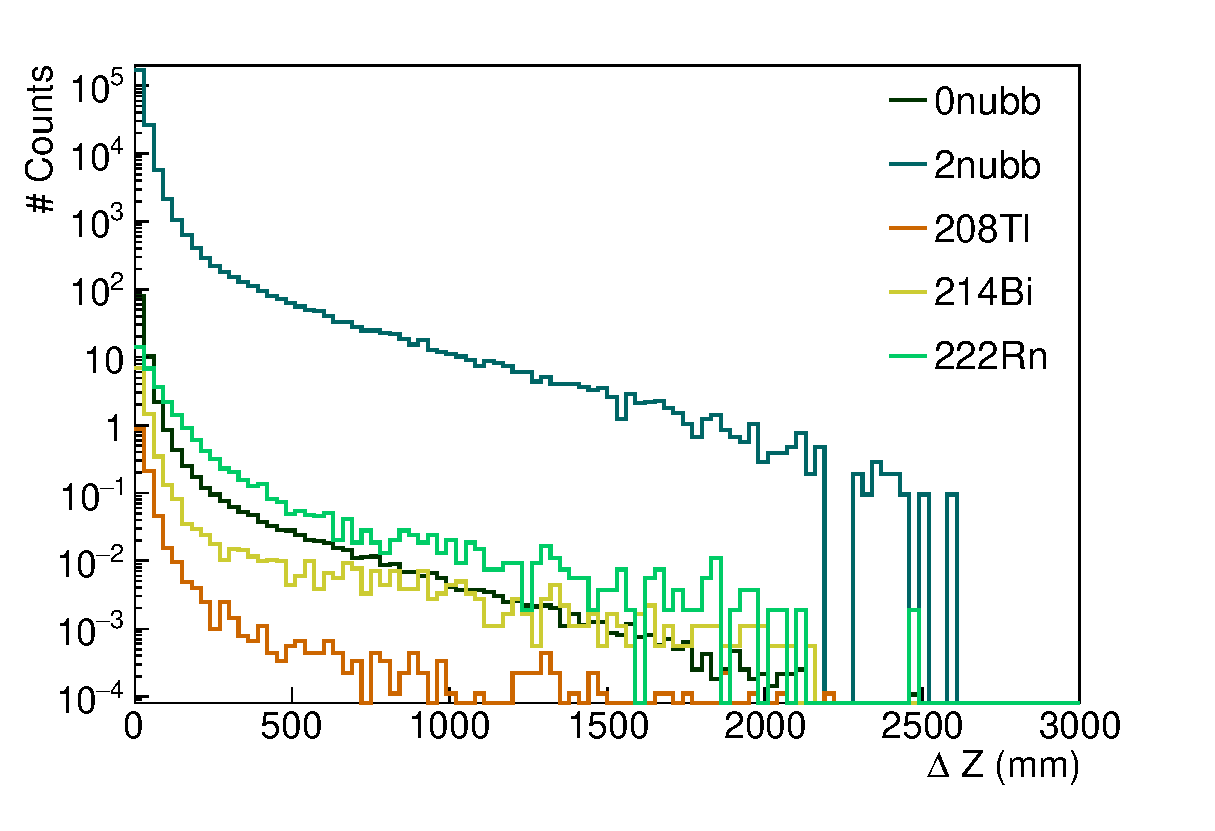
\includegraphics[width=0.8\textwidth]{Sensitivity/fig_sensitivity/Vertex_distance.eps}
  \caption{
    \label{fig:vertex_dist}}
\end{figure}
The two electrons of $\zeronu$ and $\twonu$ decays are actually emitted from the same vertex, unlike natural isotope disintegrations.
* a finir*

Fig.~\ref{fig:cont_vertex} displays the limit set on $\Tbeta$ as a function of the applied cut-off on the vertex distance in the Z direction.
\begin{figure}[h]
  \centering
  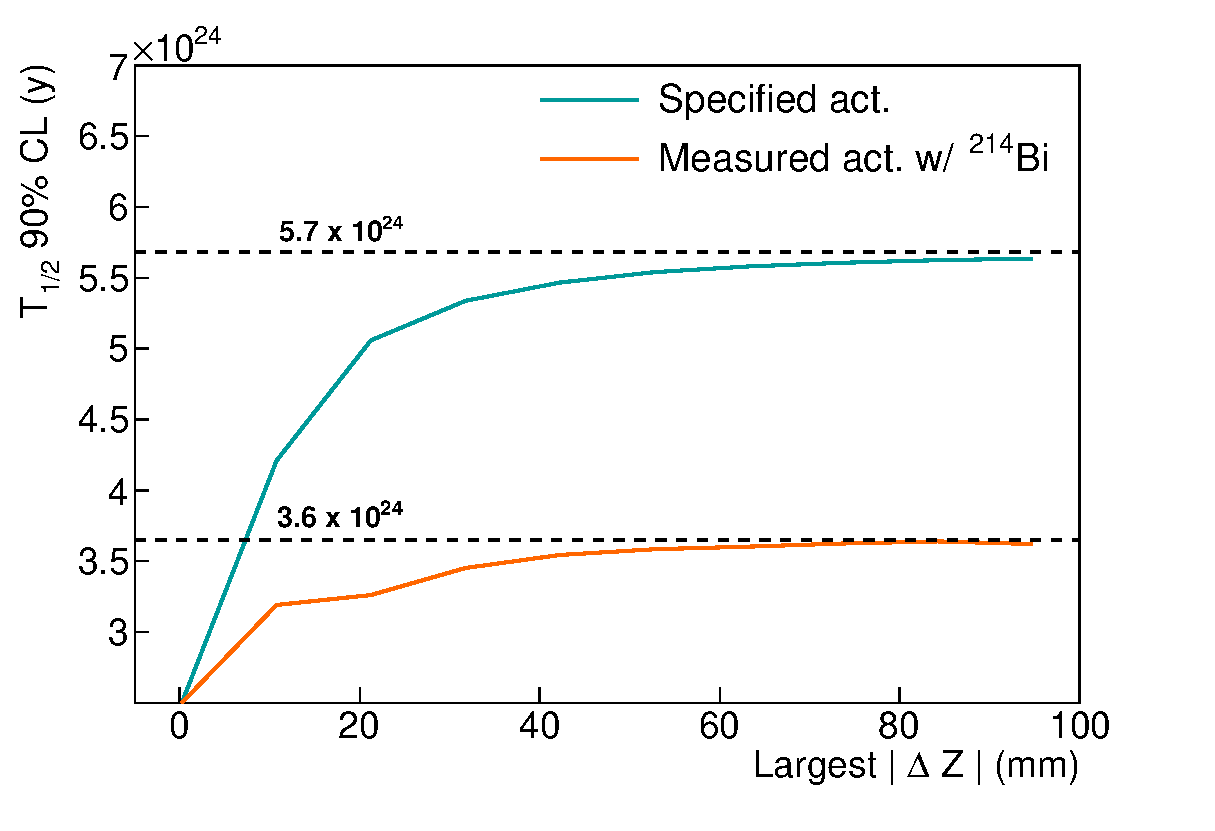
\includegraphics[width=0.8\textwidth]{Sensitivity/fig_sensitivity/contamination_vertex.eps}
  \caption{
    \label{fig:cont_vertex}}
\end{figure}
For all three contamination levels, we reach a plateau for a cut-off of more than 60 mm in $\Delta z$.
The same conclusions apply to the $\Delta y$ cut-off.
These results are consistent with the findings of the previous analysis conducted by Steven Calvez, asserting the two reconstructed vertices on source foils should not be separated by more than $60$ mm horizontally ($|\Delta y| < 60$ mm), and by more than $70$ mm vertically ($|\Delta z| < 70$ mm).


These cuts follow the NEMO-$3$ analysis on the background rejection, whose effectiveness were lately confirmed for the SuperNEMO demonstrator~\cite{docdb:calvez2014}.
first-order and topological cuts have efficiencies of selection differing for each type of decay.
We computed these efficiencies, presented in Tab.~\ref{tab:selections_eff}.
\begin{table}[h]
  \centering
  \begin{tabular}{|c|c|c|c|}
    \hline
    & first-order cuts (\%) & Internal probability (\%) & Vertex distance (\%)  \\
    \hline\hline
    $\zeronu$  & $26.9$ & $25.3$ & $24.2$ \\
    $\twonu$  & $9.16$ & $8.57$ & $8.01$ \\ %% (à recalculer avec 2nu2mev)
    \Tl  & $0.106$ & $0.0888$ & $0.0821$\\
    \Bi  & $0.168$ & $0.151$ & $0.140$ \\
    \Rn  & $0.0169$ & $7.3\times 10^{-5}$ & $4.27\times 10^{-5}$\\
    \hline
  \end{tabular}
  \caption{Number of selected $2e$ topologies compared with the total number of simulated decays, for first-order cuts and topological cuts.
  \label{tab:selections_eff}}
\end{table}
We observe topological cuts allow the selection of a high proportion of $\zeronu$ signal events, while rejecting most of the background events, especially the Radon-induced \Bi\ decays inside the tracker.
%% As explained in Sec.~\ref{sec:sensitivity_simus}, the \Bi\ decays following a Radon contamination of the tracker are not emitted from the source, but mainly from the tracker wires.
%% The internal probability and vertices separation can therefore help discriminate such events from signal events.

After looking at the effect of contaminations on the sensitivity, we review the influence of the magnetic field inside the detector.


\section{Impact of the magnetic field on the sensitivity}


The SuperNEMO demonstrator was originally designed with a copper coil, similarly to NEMO-$3$, delivering a magnetic field inside the tracker volume, aiming to provide an electron/positron discrimination.
This $25$~G magnetic field is high enough to bend the trajectory of the few MeV electrons and positrons of interest for SuperNEMO, without preventing them from reaching the calorimeter.
In practice, this magnetic field is mainly used to identify and reject the electron-positron pairs created by high energy $\gamma$’s, themselves emitted after a neutron capture.
In this study, however, we did not consider the contribution of external background in determining the best sensitivity.
We will therefore focus on evaluating the influence of the presence of the magnetic field on the rejection of internal and wire chamber backgrounds.
%% It is also very useful to better identify the crossing electron events, mostly coming from a 212 Bi contamination on the surface of the calorimeter, as explained in Section 3.2.4.
%% For instance, as shown in Figure 4.1, NEMO-3 observed three events in the [2.8;3.2]MeV region of interest in the one electron one positron channel and two events, induced by high energy $\gamma$’s from neutron capture, with energies higher than 4 MeV.


%% As described in Sec.~\ref{sec:magnetic_field}, the presence of a magnetic field of $25$ G could influence the optical modules performances.
%% In the simulated detector, such effects are not yet implemented, therefore can't be observed in the framework of this analysis.
%% However, possible degradation of the event reconstruction efficiency.



\subsection{Simulations of the magnetic field inside the demonstrator and reconstructed track fit}

In order to study the influence of the magnetic field on the Selenium-$82$ $\zeronu$ sensitivity, the simulations and reconstructions of decays described in Sec.~\ref{sec:sensitivity_simus} have been performed in three different conditions:
\begin{itemize}
\item simulations with a $25$ G \emph{uniform} magnetic field (following recommendations \cite{CalvezThesis}),
\item simulations where the magnetic field is turned off,
\item simulations with a $25$ G \emph{mapped} magnetic field, taking into account more realistic variations of the magnetic field inside the detector~\cite{docdb:map_magnetic_field2015}.
\end{itemize}
Each magnetic field condition has the same number of simulated events, as summed up in Tab.~\ref{tab:sensitivity_simulations}.
Depending on the case considered, the electrons will not have the same trajectory curvature.
In the first uniform on-field case, the best track fit is performed by helices.
In the second off-field case, the motion of an electron is in a straight line.
The fitting algorithm have thus be modified to match line trajectories.
Finally, the best tracking option (line or helix) for the third mapped on-field case will be discussed in the next section.

We oppose in Fig.~\ref{fig:real_target_act} the $\Tbeta$ results with and without this field inside the detector.
A third result is also presented, with the mapped field.

\subsection{Impact of the magnetic field on signal background selections}

Among the various event selection criteria considered in Sec.~\ref{sec:sensitivity_ev_selection}, the last one is of primary importance with regard to the influence of the magnetic field on the final sensitivity of the detector.
Indeed, when the magnetic field is switched on, the charged particles of few MeV (as electrons and positrons) have a curved trajectories.
A particle is then identified as an electron when the trajectory fitting results in a negative curvature.
When the magnetic field is switched off, the trajectory of the charged particles takes place in a straight line\footnote{When we say this, we do not take into account possible deviations in the trajectory of the particles, due in particular to multiple scattering in the tracker.}.
This last selection criterion is then no longer applied.
Consequently, the number of identified $2e$ topologies, selected by the first-order cuts, are increased, for the signal and background simulated events.
To illustrate this effect, we give in Fig.~\ref{fig:eff_0nu_w_wo_B} the selection efficiency $\epsilon_{0\nu}$ as a function of the $2e$ total energy, for the two cases of magnetic field presented above.
\begin{figure}[h]
  \centering
  \includegraphics[width=0.8\textwidth]{Sensitivity/fig_sensitivity/Nbkg_field.pdf}
  \caption{The $\zeronu$ selection efficiency as a function of the $2e$ total energy, for the on-field (blue) and the off-field (orange) cases.
    The two corresponding region of interests are also displayed by coloured stripes.
    Here no optimised topological cut-offs have been applied.
    \label{fig:eff_0nu_w_wo_B}}
\end{figure}
The two coloured stripes represent the corresponding region of interests, of [$2.7$;$3.15$]~MeV for the \emph{on-field} case, and [$2.75$;$3.2$]~MeV for the \emph{off-field} case.
These results are presented for the specified contamination levels, but remain valid in all cases.
We clearly notice that, for the total energy interval [$0$;$4$] MeV, the number of $\zeronu$ events selected is higher in the off-field case, which confirms what we were saying above.

The $\zeronu$ selection efficiency in the region of interest directly impacts the final sensitivity, following Eq.~\eqref{eq:tbeta_limit}.
Indeed, the upper limit set on $\Tbeta$ depends on $\epsilon_{0\nu}$ as well as on $N_{0\nu}^{\text{excl.}}$, the number of signal events excluded.
Nevertheless, for such levels of contaminations, due to the Feldman-Cousins statistics, the latter has no effect on sensitivity, and only the $\zeronu$ selection efficiency in the region of interest plays a role.
For the two field cases of interest, these efficiencies are $\epsilon_{0\nu}^{\text{on-field}}=0.15\%>\epsilon_{0\nu}^{\text{off-field}}=0.12\%$.
The selection efficiency for the on-field case is favoured by the lower bound of the ROI.
In fact, the further this lower bound is shifted towards lower energies, the greater the selection efficiency.
Besides, slight variations of the upper bound have almost no impact.
As expected, this results in a decrease in sensitivity for the off-field case, giving
\begin{equation}
\Tbeta > 4.80\times 10^{24}\,\text{y}\qquad (90\% \text{CL})\,.
\end{equation}

However, this decrease in sensitivity when the field is switched off can be compensated by applying the topological cut-offs described in subsection~\ref{subsec:opti_ev_selection}.
We optimised these selections for each contamination level case, and for both field and no field cases.
In Fig.~\ref{fig:sensitivity_B} are presented the best values for $\Tbeta$, using optimised topological cut-offs, both for on-field (see Tab.~\ref{tab:cut_Pint}) and off-field cases.
\begin{figure}[h]
  \centering
  \includegraphics[width=1.1\textwidth]{Sensitivity/fig_sensitivity/contamination_Se_w_woB.pdf}
  \caption{Best limit set on $\zeronu$ half-life (top pad), and the corresponding ROI (bottom pad), as a function of the contamination level considered, for both on-field and off-field cases.
    \label{fig:sensitivity_B}}
\end{figure}
The topological cuts allow to increase the final sensitivity.
The $\Tbeta$ value for off-field case, taking the specified activities, goes from $4.80\times 10^{24}\,\text{y}$ to $6.22\times 10^{24}\,\text{y}$, an improvement of $30\%$.
Because of the higher level of selected $2e$ topologies, higher sensitivities can be reached for the off-field case than for the on-field case, if using optimised topological cut-offs.
More generally, by using first-order cuts as well as topological cuts adapted to each case, we achieve higher sensitivities for the off-field case.
We note, however, that for high contamination levels (i.e. measured activities with and without bismuth), the difference in sensitivity for the two magnetic field cases tends to decrease.

\subsection{Influence of the magnetic field on optical modules and reconstruction efficiency}

Studies have been lead to evaluate its influence on the optical modules and on the event reconstruction~\cite{CalvezThesis}\cite{internal:magnetic_field}.

SuperNEMO PMTs are protected from the external magnetic field by an iron shield.
Unfortunately, the latter do not perfectly protect the PMTs, and a residual magnetic field is measured inside the shieldings, leading to charge losses and worsened energy resolution.
It was shown that applying a $25$ G magnetic field, and protect the PMTs with iron magnetic shields would be optimal, but not without consequences.
In fact, for the recommended value of $25$ G for the magnetic field, PMT charge losses would be close to $8\%$, and the PMT energy resolution would be increased of $\sim 3\%$.
Moreover, the PMTs shieldings could themselves severely impact the shape of the field lines, as well as its strength.
In fact, with a $25$ G magnetic field generated by the copper coil, the magnetic shields are responsible for the field strength decreasing, and barely $10$ G is expected near the source foils.
Moreover, the magnetic field strength decreases quickly as we get closer to the calorimeter walls.
The reconstruction efficiency could therefore be greatly impacted:
the magnetic field intensity varying from the source foils to the calorimeter wall, electrons trajectory curvatures are not constant, and the track is less well fitted.
This effect is higher as the electron energy decreases.

Despite the fact that magnetic shields were designed and installed to protect the PMTs, this field can have a great impact on the calorimeter detection efficiency, and thus could degrade the detector's sensitivity to the $\zeronu$ decay.
If the studies cited have evaluated the influence of the presence of the magnetic field on the reconstruction efficiency of $\zeronu$ events, it remains to be seen its consequences on the final demonstrator sensitivity.



\section{Searching for the Neodymium-$150~\zeronu$ decay}
\label{sec:Nd}

This study was conducted jointly with the PhD student Axel Pin, from CENBG~\cite{}.
Although we both worked on the whole of the analysis, I presented in detail, in the previous sections, the results regarding the influence of the magnetic field.
Meanwhile, Axel Pin will present in detail the possibility of changing the Selenium material by Neodymium sources~\cite{AxelThesis}.
The current section aims at summarise the feasibility study on Neodymium sources.

In the case SuperNEMO demonstrates the feasibility of a large-scale tracko-calo experiment, we would examine the possibility of different source isotopes, as done on NEMO-$3$.
The \Nd\ has a more favourable $\Qbb$ than \Se, with $\Qbb = 3.37$ MeV, .
However, its $\Ttwonu$ is lower, with $9.1\times 10^{18}$~years [ref].
For this study, we keep the \Se\ values for the contaminations, despite different purification efficiencies for the two isotopes.


\begin{itemize}
\item préciser que compte-tenu du Z important du 150Nd, même si la demi-vie de la 2nu est assez faible, cela ne gêne pas trop car les effets coulombiens font que la 2nu ne contribue pas trop à haute énergie.
\item distribution t1/2 avec différents échantillons de simus (17.5 kg.y)
\end{itemize}

\section{The final detector sensitivity}

The final goal of the SuperNEMO demonstrator is to demonstrate that the NEMO technology is scalable to reach high half-life sensitivity on the $\zeronu$ decay.
It was therefore mandatory to study the case of the final detector sensitivity, consisting in building $20$ modules similar to the SuperNEMO demonstrator, to reach unprecedented levels on effective neutrino masses.



\section{Conclusion}
\begin{itemize}
\item Etude plus générale avec bkg externe+lab (reprendre chiffres NEMO3) + neutrons (cf NEMO3)
\item Plot général récap tous résultats
\item delayed cells->improvement, cf NEMO 3
\item ouverture sur possibilité d'étudier l'influence de la résolution en temps des PMs sur l'eff des coupures (Pint)
\item cellules tracker dead-> refaire analyse
\item manque de stat pour le neodyme car ROI haute E
\item légères diff avec résultats axel car légères diff dans sélections d'ev car utilisation PID
\item tenir compte de la dégradation en énergie dans les simus du au B
\item optimisation topo cuts : multivariate analysis peut être envisagée pour aller plus loin
\end{itemize}

               \chapter{Improvement of the internal Thallium-$208$ background rejection}
\label{ch:timediff}

At the end of September $2018$, the $34$ enriched-Selenium source foils were installed on the demonstrator.
At this time, the internal \Tl\ and \Bi\ activities of these sources had already been measured by the BiPo detector.
Also, the Radon concentration in the chamber was extrapolated from Radon emission measurements of the tracker components with a concentration line for an incoming gas flow of $2$~m$^{3}$/h.
We described in the previous chapter the impact of these activities on the final detector sensitivity to the $\zeronu$ decay, and set up optimised topological selections adjusted to reject the Radon background.

However, \Tl\ disintegrations in the sources also remains a troublesome background, even for $\beta\beta$ emitters with a high $\Qbb$.
Indeed, it contributes at high energies (up to $4$~MeV on the two electrons energy sum spectrum), because of the internal conversion of the $2.615$~MeV $\gamma$-ray.
In a context where the \Tl\ contamination is higher than expected inside the sources, we focus in the current chapter on rejection techniques peculiarly adapted to reject internal \Tl\ events.
We study the influence of these additional techniques on $\zeronu$ events selection, and evaluate the impact on final detector sensitivity.
Impact of the calorimeter timing performances on these techniques are also addressed in this chapter.

\section{Motivations}

In Chapters~\ref{ch:detector} and \ref{ch:sensitivity}, we presented the specifications set on the background activities, in order to reach the target limit on the $\zeronu$ process half-life of the \Se\ in $5$ years, with $100$~kg of isotope.
The Tab.~\ref{tab:real_target_act} given in Chapter~\ref{ch:detector} summarises the target \Tl, \Bi\ and \Rn\ activities, and provides a comparison with those measured by the collaboration.
The BiPo detector was capable of giving an upper limit on the \Bi\ level of ${\mathcal{A}^{\text{Bi}}<290~\mu}$Bq/kg at $90$\% CL, and future more precise measurements with SuperNEMO demonstrator will constraint this value.
The BiPo measurements also showed that the \Tl\ contamination is about $30$ times greater than expected on average.
We give in Tab.~\ref{tab:Nbkg_wBi} the number of expected background events for the measured activities (taking the upper limit for \Bi\ contamination), for the demonstrator and final detector.
\begin{table}[!h]
  \centering
  \begin{tabular}{|c|c|c|}
    \hline
    Exposure & Demonstrator & Detector  \\
    & $17.5$~kg.y & $500$~kg.y \\
    ROI (MeV) & [$2.7$;$3.3$] & [$2.6$;$2.95$] \\
    \hline\hline
    $\twonu$  & $0.383$ & $104$  \\
    \Tl  & $1.09$ & $21.2$  \\
    \Bi  & $1.42$ & $110$  \\
    \Rn  & $0.0782$ & $6.11$  \\
    \hline
  \end{tabular}
  \caption{Expected number of background events in the $2e$ topology, in optimised energy ranges for the SuperNEMO demonstrator ($17.5$~kg.y) and the final detector ($500$~kg.y exposure).
    The $\twonu$ half-life is taken as $\Ttwonu~=~9.39\times~10^{19}$~y, and the measured background activities are considered (with the upper limit for \Bi\ contamination).
    The topological selections have been optimised: \Pint$>4$\% and $|\Delta~Z|~<~80$~mm.
    ROI are optimised to maximise the $\Tbeta$ limit at $90$\% (see Chapter~\ref{ch:sensitivity}).
    \label{tab:Nbkg_wBi}}
\end{table}
With an activity fixed to the measured one, the \Tl\ background does not affect significantly the sensitivity of the demonstrator ($17.5$~kg.y exposure) as only one event is expected in the optimised [$2.7$;$3.3$]~MeV energy region, after first-order and topological cut-offs were applied.
On the other hand, this background could be harmful for the final detector ($500$~kg.y exposure), with $21$ events expected in the region of interest [$2.6$,$2.95$]~MeV.
To overcome this effect, it is interesting to set a specific method designed to reject \Tl\ events.

In the next section, we describe the specific features of the Thallium internal background.
We develop a new technique of rejection, especially designed to identify internal \Tl\ events, based on several Time-of-flight computations.

\section{The internal \Tl\ background}

As described in Chapter~\ref{ch:detector}, radioactive isotope disintegrations inside the source foils can occasionally produce two-electron events, and thus can mimic $\beta\beta$-decay events.
The \Tl, a progeny of \Th, is one of the largest contribution to the internal background.
Two electrons can be produced via a $\beta$-decay followed by a M\o{}ller scattering, $\beta$-decay to an excited state with the subsequent internal conversion, or due to Compton scattering of the de-excitation photon.

The disintegration scheme of \Tl\ isotope is presented in Fig.~\ref{fig:Tl_scheme}.
\begin{figure}[!h]
  \centering
  \includegraphics[width=13cm]{timedifference/fig_timediff/Tl_decay_scheme.pdf}
  \caption{A simplified disintegration scheme for the \Tl\ isotope.
    $81$~\% of the disintegration pass through the $294$~ps metastable energy level (orange).
    All disintegration go through the $2.615$~MeV energy level (green), where an orbital electron is ejected in $0.246$~\% of the cases through the internal conversion process.
  \label{fig:Tl_scheme}}
\end{figure}
This shows that \Tl\ always $\beta$-decays to an excited state of the \Pb\ daughter nuclei.
In more than $99$~\% of the decays, at least 2 $\gamma$'s are expected after the $\beta$ emission.
For $\zeronu$ detection of isotopes with high $\Qbb$, the most dangerous mode of $\beta\beta$-like events production comes from the internal conversion of the $2.615$ MeV-$\gamma$, resulting in one electron with an energy of $2.5$ MeV approximately and a beta-electron with a continuous spectrum between $0$ and $\sim~1.5$~MeV.
Thus \Tl\ events with a total energy greater than $2.7$~MeV can populate the region of interest.

\subsection{The internal conversion process}

An excited nucleus will practically constantly achieve a transition to a lower state by one of two processes: the emission of a $\gamma$-ray, or the ejection of one of the orbital electrons.
The latter, called \emph{internal conversion} (frequently abbreviated IC), is a second-order process, where an electron couples to a proton inside the excited nucleus.
Thus, in such a radioactive decay, the de-excitation energy of the nucleus is transferred \emph{directly} to a $j$-shell electron ($j=K,L,M...$).
A high-energy electron is therefore emitted from the atom, and carry off the energy
\begin{equation}
E_{IC} = E_{\gamma}-E_{j}\qquad (j=K,L,M...)\,,
\end{equation}
where $E_{j}$ is the binding energy of the electron in the $j$-shell, and $E_{\gamma}$ is the energy of the $\gamma$-ray.

This mechanism is possible because there is a non-zero probability of finding the electron within the nucleus, that is to say, the wave-function of the electron can penetrate the volume of the nucleus.
Consequently, due to their high nuclear penetration, electrons coming from the $1s$ state are more likely to be ejected (this transition is called $K$ internal conversion).
Although electrons coming from $2s$, $3s$ and $4s$ states ($L$, $M$ or $N$ internal conversions) have also a non-zero probability to undergo this process.
After the electron ejection, the hole in the corresponding shell is filled by an electron from a higher energy level, emitting characteristic $X$-rays, Auger electrons, or both.

For a given transition, the internal conversion coefficient of the electron in the $j$-shell, is defined by
\begin{equation}
\alpha_{j}=\frac{P_{IC, j}}{P_{\gamma}}\,,
\end{equation}
%% \begin{equation}
%% \alpha_{K}=\frac{P_{IC, K}}{P_{\gamma}}\,,
%% \end{equation}
where $P_{IC,j}$ is the $j$ conversion electron emission probability, and $P_{\gamma}$ is the $\gamma$-ray emission probability.
The total coefficient is
\begin{equation}
  \alpha_{T}=\sum_{j=K,L,M\cdots}\alpha_{j}\,.
\end{equation}
These coefficients are given in Tab.~\ref{tab:IC_prob} for the $2.615$~MeV energy level of \Tl\ isotope.
\begin{table}[!h]
  \centering
  \begin{tabular}{|c|c|c|c|c|}
    \hline
    $j$-shell & $K$ & $L$ & $M$ & Total \\
    \hline\hline
    IC coefficients (\%) & $0.1708$ & $0.0292$ & $0.00685$ & $0.246$ \\
    \hline
  \end{tabular}
  \caption{Internal conversion coefficients for the $2.615$~MeV $\gamma$-ray of the \Tl\ decay scheme.
    \label{tab:IC_prob}}
\end{table}
Therefore, in $0.246$~\% of the cases, the \Pb\ excited nucleus will undergone an internal conversion corresponding to the $2.615$~MeV energy level.


\subsection{\Tl\ disintegrations in the 2e channel}

Finally, a \Tl\ decay can present a two-electrons topology when, after the $\beta$ emission, an electron is ejected from the atom through internal conversion.
Especially, when this energy transfer corresponds to the $2.615$~MeV $\gamma$-ray, the ejected electron carry off a significant energy, depending on its initial binding energy with the nucleus.
For instance an orbital electron from the $K$-shell is ejected with an energy $E_{IC,K}=2.526$~MeV (${\alpha_{K}=0.17}$\%).
This decay is therefore likely to contribute in the region of interest for the $\zeronu$ search of \Se, or even \Nd.

%% In Fig.~\ref{fig:Emin_Emax_Tl} is presented the individual energy spectra for $2e$ topologies for \Tl\ simulations inside the source foils.
%% \begin{figure}[!h]
%%   \centering
%%   \includegraphics[width=13cm]{timedifference/fig_timediff/energy_spect_min_max_208Tl.pdf}
%%   \caption{Individual energy spectra for selected $2e$ topologies of \Tl\ decays simulated inside the source foils.
%%     Calorimeter hit of minimal energy (red) and maximal energy (blue).
%%     Spectra are arbitrarily normalised.
%%     The [$2.7$;$3.2$] ROI is represented by grey dashed lines.
%%     \label{fig:Emin_Emax_Tl}}
%% \end{figure}
%% An usual technique to reject \Tl\ background consists in distinguishing $2e$ topologies for which one of the two calorimeter hit has an energy greater than $2.7$~MeV.
%% The energy resolution of the demonstrator being improved by a factor of $\sim~2$ with respect to NEMO-$3$, this selection is efficient.
%% This cut-off allows to reject $0.61$~\% of the \Tl\ internal events, while rejecting only $0.11$~\% of $\zeronu$ events.

In the $2e$ channel, optimised topological cut-offs, based on time-of-flight computation and the distance between vertices, were presented in the previous chapter.
They are mostly efficient in rejecting the non-internal \Rn\ events.
After a brief presentation of the simulations carried out as part of this analysis, we remind and specify the internal probability computation, and present a new selection, also based on the time-of-flight computation, to reject the \Tl\ background.

%% \begin{itemize}
%% \item donner la proportion d'ev retardés avec la bank SD (simus en train de tourner)
%% \item relire et compléter cette sous-section
%% \item Avant d'entrer dans le détail préciser le principe de la réjection par temps de vol.
%%   L'électron de plus haute énergie est en retard, avec un retard en moyenne de 294 ps pour la plupart des niveaux (discuter un peu le schéma de désintégration, dans quel cas il sera en retard).
%%   Ensuite dire que tu as quantifié le pourcentage d'électrons de haute énergie en retard avec une simulation "parfaite" i.e. avec une résolution en  temps  nulle.
%%   A comparer avec le chiffre donné précédemment (issu d'une étude du schéma de désintégration.)
%% \end{itemize}


\section{Simulated demonstrator performances}

The background model used in the framework of this study has already been described in detail in the previous chapter.
Nevertheless, calorimeter performances implemented in the Falaise software have been modified in this study.
Indeed, one of the main goal is to evaluate the influence of the calorimeter timing performances on the \Tl\ background rejection.
This study was led before the commissioning phase of the calorimeter when timing performances were characterised only for few optical modules, and before their installation at Modane~\cite{HuberThesis}.
An encouraging value for the uncertainty on the calorimeter time measurement of $248.3$~ps for incoming electrons and $341.8$~ps for photons were provided for the best optical module tested (Fig.~\ref{fig:Arnaud_RMS_PM}).
\begin{figure}[!h]
  \centering
  \includegraphics[width=13cm]{timedifference/fig_timediff/Arnaud_RMS_PM.pdf}
  \caption{Time distribution of the trigger time of an optical module in the case of electrons (red) and gamma radiation (green) depositing an energy of $1$~MeV in the scintillator.
    The trigger threshold is set at $45$ mV and corresponds to an energy of $0.150$~MeV.
    Adapted from~\cite{HuberThesis}.
  \label{fig:Arnaud_RMS_PM}}
\end{figure}
In this context, before the full calorimeter calibration in Modane, we would give an overview of the influence of these performances on the \Tl\ background rejection.
To do so, signal and background simulations were performed supposing the optical modules measure perfectly the particle time-of-flights, by setting to zero the time uncertainty at the level of the calibration module in the Falaise pipeline.
I wrote a Root code allowing to degrade the precision on time measurements for it to be set by the user to the desired accuracy.

All of the simulations produced for this analysis were generated using the official Falaise pipeline, and are made available to the collaboration in the common SuperNEMO repository at the IN$2$P$3$ computing centre platform.
The same code described in the previous chapter has been used for this study, including the Particle Identification module, the module I wrote and the Root code pipeline.
An additional set of codes have been developed in order to degrade the simulated calorimeter resolution as well as to compute the analysis tools described in the following.

In the first instance we set the reasonable value of $200$~ps for the measurement uncertainty.
In Sec.~\ref{subsec:calo_sigma} the influence of this parameter on the \Tl\ rejection is provided, and we give final sensitivity results according to it in Sec.~\ref{sec:Tl_sensitivity}.


\section{Rejection of \Tl\ with a time-of-flight criterion}
\label{sec:Tl_TOF}


The internal probability, based on time-of-flight computation, quantifies the likelihood that two particles were emitted inside the source foils, from the same vertex.
Unless it is a useful tool, we would implement a new one, also based on time-of-flight, taking into account the possible delay between the two incoming electrons due to the \Pb\ metastable state.

%% Internal conversion occurs after $\beta$ or $\alpha$ radioactive decays leaving the nucleus excited.
%% Then a $\gamma$ particle is emitted and transfers its energy to an atomic electron which results in ejection of this electron from the atom.
%% The emitted electron has an energy corresponding to the energy of previously excited nucleus reduced by the electron binding energy.
%% After the internal conversion, electrons reorganise.
%% The hole in internal layer is filled by an electron from an external layer (emitting an X ray).\\
%% The probability for an atomic electron to be ejected decreases with the initial binding energy.
%% Thus, electrons from K layers have a higher probability to be converted (see Fig.~\ref{fig:Tl_IC}).

\subsection{The internal probability}

As part of the analysis pipeline, this tool is widely employed in NEMO-$3$ and SuperNEMO, for background rejection purposes.
We present it in detail in Chapter~\ref{ch:detector} and examine an example of its usefulness in Chapter~\ref{ch:sensitivity}.
Nevertheless, in the framework of this analysis we need to perform our own calculation of internal probability, after the reconstruction pipeline, because the simulations are performed for an ideal value of the optical module performances.
That is an opportunity to come back to this tool and to clarify certain points.

The calculation of the internal $\chi^{2}$ is reminded in Eq.~\eqref{eq:int_chi2_electrons}, for two detected electrons, as a function of the expected time-of-flights, $t^{\text{exp}}$, the experimentally measured time-of-flights, $t^{\text{meas}}$, as well as the total uncertainty on the time-of-flight measurement:
\begin{equation}
  \chi^{2}_{int}=\frac{((t^{\text{meas}}_{1} - t^{\text{exp}}_{1}) - (t^{\text{meas}}_{2} - t^{\text{exp}}_{2}))^{2}}{\sigma_{t_{1}}^{2}+\sigma_{t_{2}}^{2}+\sigma_{\beta_{2}}^{2}+\sigma_{\beta_{1}}^{2}+\sigma_{l_{1}}^{2}+\sigma_{l_{2}}^{2}}\,.
  \label{eq:int_chi2_electrons}
\end{equation}
$\sigma_{t_{i}}$ is the uncertainty on the measured time-of-flight.
$\sigma_{\beta_{i}}$ and $\sigma_{l_{i}}$ are the uncertainties on the expected time-of-flight brought by the uncertainty on particle energies and track lengths, respectively.
The denominator square root corresponds to the total uncertainty, whose measured time-of-flight uncertainty is simulated as zero and degraded afterwards.

In the official SuperNEMO reconstruction pipeline, ${\sigma_{l}=\sigma_{l_{1}}=\sigma_{l_{2}}=70}$~ps for electron particles.
As we simulated perfect calorimeters, we check that this parameter is correctly evaluated in order to implement it in our own off-line Root code pipeline.

\subsubsection*{Optimisation of $\sigma_{l}$}

One way to examine if $\sigma_{l}$ is well-evaluated is to look at the flatness of the internal probability distribution for $\zeronu$ events in the $2e$ topology, for which a flat distribution is expected.
Indeed, the slope of this distribution provides pertinent information to check the estimation of uncertainties.
The flatter the distribution, the more correctly uncertainties are estimated.

Therefore, for this optimisation, we use $2e$ topologies of signal simulations inside the source foils.
Discrete values of $\sigma_{l}$ running from $0.01$ to $0.1$~ns are used to compute the internal probability distributions of these events.
For each distribution, a linear fit is performed on the reduced range \Pint$~\in[0.1;1]$ in order to avoid the peak at low internal probabilities.
The \emph{flatness parameter} $a_{F}$ is defined as the slope parameter of the linear fit.
The optimisation then consists in finding the value of $\sigma_{l}$ for which the parameter $a_{F}$ is cancelled, which corresponds to the best estimate for $\sigma_{l}$.

In Fig.~\ref{fig:flatness} is given the slope $a_{F}$ as a function of $\sigma_{l}$.
\begin{figure}[!h]
  \centering
  \includegraphics[width=13cm]{timedifference/fig_timediff/flatness.pdf}
  \caption{Slope $a_{F}$ as a function of the time uncertainty due to the reconstructed track length $\sigma_{l}$.
    The former value used in the SuperNEMO reconstruction pipeline is pointed out by blue dashed lines.
    The value kept for $\sigma_{l}$ is the one for which $a_{F}=0$, $\sigma_{l}~=~27.8~\pm~0.8$~ps, showed by purple dashed lines.
    \Pint\ is calculated for $\zeronu$ decays simulated inside the source foil, with first order cut-offs applied.
    \label{fig:flatness}}
\end{figure}
For $\sigma_{l}=70$~ps, $a_{F}>0$, revealing an overestimation of uncertainties in the computation of the internal $\chi^{2}$ in the SuperNEMO reconstruction pipeline, at the Particle Identification module level.
The optimised value, kept for the further analysis, is $\sigma_{l}~=~27.8~\pm~0.8$~ps.
In Fig.~\ref{fig:Pint_comparison} is displayed the internal probability distributions for these two values of the $\sigma_{l}$ parameter, $\sigma_{l}=70$~ps and $\sigma_{l}=27.8$~ps.
\begin{figure}[!h]
  \centering
  \includegraphics[width=13cm]{timedifference/fig_timediff/Pint_comparison.pdf}
  \caption{Internal probability distributions for $\sigma_{l}=70$~ps (blue) and $\sigma_{l}=27.8$~ps (green).
    \Pint\ is calculated for $\zeronu$ decays simulated inside the source foil, with first order cut-offs applied.
    \label{fig:Pint_comparison}}
\end{figure}

Let us notice that normally $\sigma_{l}$ should depend on the track length as well as the energy, especially as multiple scatterings in the tracker have a more notable impact for low energy electrons.
A more complete analysis would then compare the simulated track lengths with the reconstructed ones, for different energy simulated sets of mono-kinetic electrons, to evaluate this dependence.
Nevertheless, our optimisation is good enough for the current analysis.
Discussions are in progress to modify this parameter in the SuperNEMO software.

The internal probability is principally designed to reject non-simultaneous events coming from the source foils.
Therefore, it is extremely effective in rejecting \Rn\ events produced far from the source foils.
Even if it is less, this criterion is also effective in rejecting \Tl\ events, due to the existence of a metastable state for the daughter nucleus of \Tl.
Therefore the emission of the $2.615$~MeV-$\gamma$ is in most of the cases delayed.
But to describe even better these internal conversion events we would set up a new probability law expressing the hypothesis that a given event is from a $\beta$+IC delayed \Tl\ disintegration.

\subsection{The exponential probability for \Tl\ events}

According to the disintegration scheme of the \Tl\ isotope (Fig.~\ref{fig:Tl_scheme}), there is an $81~\%$ probability of passing through the $294~$ps metastable level.
After that, to reach the ground state of \Pb, the excited nucleus has $100\%$ of probability to decay through the $2.615$ MeV energy level.
At this occasion, in $0.246\%$ of cases (Tab.~\ref{tab:IC_prob}), one of the orbital electrons is ejected from the atom following the internal conversion process.
To summarise, for $0.20$~\% of the total \Tl\ decays, a $\beta$ particle is emitted, and a delayed orbital electron is ejected through internal conversion of the $2.6$ MeV-$\gamma$.
Furthermore, $X$\% of the events with an energy sum greater than $2.7$~MeV (the ROI low bound) are from delayed internal conversion decays and could be harmful for the $\zeronu$ search.
We aim to use this delayed electron to discriminate \Tl\ internal background from the $\zeronu$ signal.

%% \begin{itemize}
%% \item relire cette partie quand les simus sont finies
%% \end{itemize}

\subsubsection{Probability density function}

For a given detected $2e$ topology, we define the $\Delta t^{meas}$ parameter as
\begin{equation}
  \Delta t^{meas} = t_{1}^{meas}-t_{2}^{meas}\,,
  \label{eq:time_diff}
\end{equation}
where $t_{1}^{meas}$ and $t_{2}^{meas}$ are the two measured time-of-flights, where $t_{2}$ stands for the electron of lowest energy, and $t_{1}$ for the one of highest energy.
If this $2e$ topology corresponds to a delayed \Tl\ event, then the electron of lowest energy is supposed to be a $\beta$ particle and the one of highest energy an electron coming from an internal conversion, delayed in average of $294$~ps.
Assuming an ideal calorimeter perfectly measuring time-of-flights and energies, the $\Delta t$ distribution for such delayed events would be a decreasing exponential, with the decay parameter ${\tau=294}$~ps.
However, in actual conditions, this exponential is degraded by the uncertainties on time-of-flight measurements detailed in Eq.~\eqref{eq:int_chi2_electrons}.
These are embedded by a Gaussian distribution centred around ${\mu=0}$~ps with a given width $\sigma$.
Therefore, to each $2e$ topology is associated a probability density function which is the convolution between an exponential and a Gaussian distribution, written down as ${(E \otimes G)_{\tau,\mu,\sigma}(\Delta t)}$.
The corresponding value of $\Delta t^{meas}$ is then found somewhere on this distribution, and will serve us to define the so-called \emph{exponential probability}, $P_{exp}(\Delta t^{meas})$, which is the probability that this event comes from a $\beta$+IC delayed decay.

%% \begin{itemize}
%% \item Du coup mettre une distribution de ces ev sur l'exponentielle quand les simus seront finies
%% \end{itemize}

\subsubsection{Exponential probability}

We wish to define this probability following the same principle as for the internal probability, for comparison purposes.
Therefore, we would obtain the maximal value ${P_{exp}=1}$ when the value of $\Delta t$ is the most probable, i.e. when $\Delta t$ is of the order of the mean of the ${(E \otimes G)_{\tau,\mu,\sigma}(\Delta t)}$ distribution.
On the other hand, minimal values for $P_{exp}$ would be reached for less probable values of $\Delta t$, so ${P_{exp} \xrightarrow[|\Delta t| \rightarrow +\infty]{} 0}$.
To do so, the ${(E \otimes G)_{\tau,\mu,\sigma}(\Delta t)}$ distribution is normalised and the exponential probability is defined as
\begin{equation}
  P_{exp}(\Delta t^{meas}) = \int_{-\infty}^{\Delta t^{meas}} (E \otimes G)_{\tau,\mu,\sigma}(t)\, dt + \int_{\Delta t_{sym}^{meas}}^{-\infty} (E \otimes G)_{\tau,\mu,\sigma}(t)\, dt\,,
  \label{eq:Pexp}
\end{equation}
where $\Delta t^{meas}_{sym}$ is defined such that ${(E \otimes G)_{\tau,\mu,\sigma}(\Delta t^{meas}_{sym})} = {(E \otimes G)_{\tau,\mu,\sigma}(\Delta t^{meas})}$.
A graphical representation is given in Fig.~\ref{fig:Pexp}.
\begin{figure}[!h]
  \centering
  \includegraphics[width=13cm]{timedifference/fig_timediff/proba_expo_test.pdf}
  \caption{Normalised convolution distribution ${(E \otimes G)_{\tau,\mu,\sigma}(\Delta t)}$.
    The parameters are $\tau=294$~ps, $\mu=0$~ps and $\sigma=\sigma_{tot}$, computed with $\sigma_{l}=27.8$~ps and $\sigma_{t}=200$~ps.
    \label{fig:Pexp}}
\end{figure}
In this example the distribution corresponds to ${(E \otimes G)_{\tau,\mu,\sigma}(\Delta t)}$ with ${\tau=294}$~ps and ${\mu=0}$~ps and the total time uncertainty is calculated taking $\sigma_{l}=27.8$~ps and $\sigma_{t}=200$~ps for $1$~MeV electrons.
The two integrals whose sum is given in the Eq.~\eqref{eq:Pexp} are represented by two red-coloured areas.
As explained, each probability density function is defined for a single $2$-electrons event, because the time-of-flight uncertainty depends on the electron measured energy and on the track length.
In the given example, we considered two particles interacting inside the calorimeter with an energy of $1$~MeV each.

In fig.~\ref{fig:Pexp_Tl} are presented exponential probability distributions for $2e$ topologies selected of \Tl\ and $\zeronu$ simulations inside the source foils.
\begin{figure}[!h]
  \centering
  \includegraphics[width=13cm]{timedifference/fig_timediff/proba_expo_400.pdf}
  \caption{Exponential probability distribution for \Tl\ (orange) and $\zeronu$ simulations (blue), for $2e$ topologies with an electron energy sum greater than $2.7$~MeV (discussed in Sec.~\ref{sec:ev_selection}).
    $\sigma_{t}=200$~ps, $\sigma_{l}=27.8$~ps.
    \label{fig:Pexp_Tl}}
\end{figure}
As expected, the distribution is flat, since this probability was defined in the same way as the internal probability.
%%The distortion at low $P_{exp}$ comes from the proportion of events where the second electron doesn't come from the internal conversion of the $2.615$~MeV $\gamma$-ray.

Now analysis tools are defined, the following sections focus on the event selections using them, the way to optimise them and their influence on the final detector sensitivity.

\section{Event selection}
\label{sec:ev_selection}


Now the exponential probability tool has been defined, the aim of this analysis is to set up events selections focusing on delayed \Tl\ events rejection.
Basic cut-offs are described, and compared with a more elaborated selection using these two probabilities.
The influence of the uncertainty $\sigma_{t}$ on time measurement is discussed at the end of the section.

\subsection{Energy selection}
\label{subsec:energy_seletion}

Based on the conclusions given in the previous chapter, the lower bound of the region of interest optimising the search of $\zeronu$ decay stands at the electron energy sum of $2.7$~MeV for the demonstrator.
From this energy, $2e$ topologies for \Tl\ are mainly populated by $\beta$ decays followed by the internal conversion of the $2.615$~MeV $\gamma$-ray.
In the following, we therefore focus only on events with a sum in energy of the two detected electrons greater than $2.7$~MeV.

\subsection{Time-of-flight cut-off}
\label{subsec:tof_cutoff}

Before using the two internal and exponential probabilities, a simple cut-off using the electron time-of-flight is explored.
Indeed, we are especially focused on rejecting the internal \Tl\ events for which the successive $\beta$ and $\gamma$-rays emissions went through the $294$~ps metastable state.
For these decays, we are expecting the particle of highest energy to be delayed compared with the one of lowest energy.
Each term in Eq.~\ref{eq:time_diff} corresponds to what it took for a particle to travel from the source to the calorimeter and depends on the time it spent in the source after emission, as well as how long it took to cross the tracker.
In order to remove from $\Delta t^{meas}$ the dependency on travel time in the tracker, we define the corrected time difference as
\begin{align}
  \Delta t^{\text{corr}} & = t^{\text{corr}}_{1} - t^{\text{corr}}_{2}\\
  & = (t^{\text{meas}}_{1} - t^{\text{exp}}_{1}) - (t^{\text{meas}}_{2} - t^{\text{exp}}_{2})\,,
\end{align}
where $t^{\text{corr}}_{i}$ are the corrected time-of-flights and $t^{\text{exp}}_{i}$ the expected ones calculated with the particle energy and track length (Eq.~\ref{eq:th_time}).

The two distributions $\Delta t^{meas}$ and $\Delta t^{\text{corr}}$ are presented in Fig.~\ref{fig:delta_t}, for $\zeronu$ and \Tl\ simulations inside the source foils.
\begin{figure}[!h]
\centering
\begin{subfigure}[t]{1.\textwidth}
  \centering
  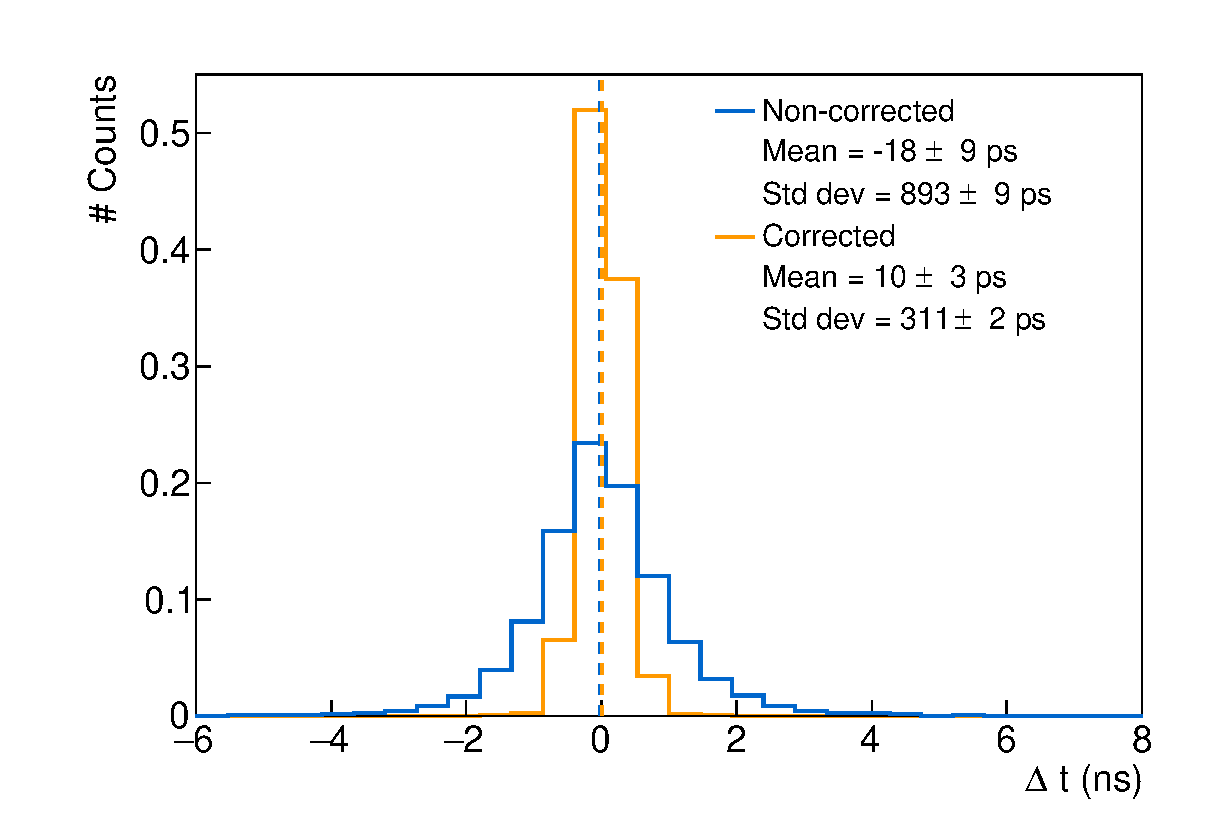
\includegraphics[width=0.7\textwidth]{timedifference/fig_timediff/0nubb_delta_t.eps}
  \captionsetup{justification=justified}
  \caption{$\zeronu$ simulations.
    \label{subfig:0nubb_delta_t}}
\end{subfigure}
\hfill
\begin{subfigure}[t]{1.\textwidth}
  \centering
  \includegraphics[width=0.7\textwidth]{timedifference/fig_timediff/208Tl_delta_t.eps}
  \captionsetup{justification=justified}
  \caption{\Tl\ simulations.
    \label{subfig:208Tl_delta_t}}
\end{subfigure}
\caption{Corrected (orange) and non-corrected (blue) time-of-flight difference between the two electrons.
  (a) $\zeronu$ simulations inside the source foils.
  (b) \Tl\ simulations inside the source foils.
  The first-order selections have been applied.
  The two distributions are normalised.
  $\sigma_{t}=200$~ps and $\sigma_{l}=27.8$~ps.
  \label{fig:delta_t}}
\end{figure}
For $\zeronu$ simulations, the $\Delta t^{corr}$ distribution is centred around zero, as the two electrons are emitted simultaneously inside the source.
Then, the correction on time difference only lowers the standard deviation of the distribution.
For \Tl\ simulations, the mean of the distribution is slightly shifted towards positive values.
Once corrected by the expected times, the mean difference between the two electrons time-of-flights stands at $296~\pm~18$~ps.
This is a direct consequence of the existence of $\beta$+IC delayed events, for which the particle of highest energy is expected to hit a calorimeter block at a time $t^{\text{corr}}_{1}~>~t^{\text{corr}}_{2}$.
The set up calorimeter time uncertainty at $200$~ps allows to be sensitive to this decay as the mean of the distribution is near $294$~ps.
Therefore, a simple way of rejecting the \Tl\ delayed events is to consider the sign of $\Delta t^{\text{corr}}$ and to reject events for which $\Delta t^{\text{corr}}~>~0$.

By applying this selection on $2e$ topologies of $\zeronu$ and \Tl\ simulations for which $E~>~2.7$~MeV, we are able to reject $76$~\% of \Tl\, while selecting $49$~\% of the $\zeronu$ ($\sigma_{t}~=~200$~ps).
The $49$\% of selected signal events is expected as the corresponding $\Delta t^{corr}$ distribution is symmetrical, unlike the one for \Tl\ events.
Although we manage to reject a significant fraction of Thallium events, the impact of this cut is too high on $\zeronu$ events.
Moreover, the uncertainties on time-of-flights are not taken into account in the rejection criterion.
Later in this chapter we consider different levels for this selection and optimise them according to the $\sigma_{t}$ value set up.
%%We study in Sec.~\ref{subsec:selection_optimisation} an optimization of this cut-off, including the influence of the temporal performance of the calorimeter $\sigma_{t}$.

\subsection{Probability cut-off}

At this level it is interesting to consider the internal and exponential probabilities to describe $2e$ topologies and attempt to obtain a higher background rejection.
They seem to be better tools notably because, unlike the $\Delta t^{\text{corr}}$ rejection criterion, they do take into account the time-of-flight uncertainties.
The first one was already used in Chapter~\ref{ch:sensitivity}, and is a widely-used tool to reject non-internal events.
The second was designed specifically for this analysis to identify delayed \Tl\ events, and also depends on the time of flight resolution through the convolution with a Gaussian function.

The idea is this section is to reject \Tl\ events taking into account their two values of internal and exponential probabilities.
Then it is interesting to represent them with a two-dimensional binned histogram of $P_{exp}$ as a function of \Pint, as done is Fig.~\ref{fig:biplot_Pexp_Pint}.
\begin{figure}[!h]
  \centering
  \includegraphics[width=15cm]{timedifference/fig_timediff/PintVSPexp_208Tl_200.eps}
  \caption{Two-dimensional histogram showing the $P_{exp}$ variations as a function of \Pint\ for \Tl\ $2e$ topologies.
    $\sigma_{t}=200$~ps and $\sigma_{l}=27.8$~ps.
    \label{fig:biplot_Pexp_Pint}}
\end{figure}
In this particular example, we picture the variations of \Pint\ and $P_{exp}$ applying ${\sigma_{t}=200}$~ps.
We clearly distinguish three event populations in this histogram.
In order to better understand these variations, we give in Fig.~\ref{fig:proba_cut_ex} three examples of ${(E \otimes G)_{\tau,\mu,\sigma}(\Delta t)}$ distributions, each of them illustrating one of the three zones.
\begin{figure}[!h]
\centering
\begin{subfigure}[t]{0.95\textwidth}
  \centering
  \includegraphics[width=0.64\textwidth]{timedifference/fig_timediff/proba_expo_1.pdf}
  \captionsetup{justification=justified}
  \caption{
    \label{subfig:Proba_cut_1}}
\end{subfigure}
\vskip\baselineskip
\begin{subfigure}[t]{0.95\textwidth}
  \centering
  \includegraphics[width=0.64\textwidth]{timedifference/fig_timediff/proba_expo_2.pdf}
  \captionsetup{justification=justified}
  \caption{
    \label{subfig:Proba_cut_2}}
\end{subfigure}
\vskip\baselineskip
\begin{subfigure}[t]{0.95\textwidth}
  \centering
  \includegraphics[width=0.64\textwidth]{timedifference/fig_timediff/proba_expo_3.pdf}
  \captionsetup{justification=justified}
  \caption{
    \label{subfig:Proba_cut_3}}
\end{subfigure}
\caption{${(E \otimes G)_{\tau,\mu,\sigma}(\Delta t)}$ distributions describing the three areas observed in Fig.~\ref{fig:biplot_Pexp_Pint}.
  (a) $\Delta t^{\text{corr}} \in~]-\infty;0]$.
  (b) $\Delta t^{\text{corr}} \in~]\Delta t_{max};+\infty]$.
  (c) $\Delta t^{\text{corr}} \in~]0;\Delta t_{max}]$.
  \label{fig:proba_cut_ex}}
\end{figure}
\begin{enumerate}
\item \Pint$\in[0;1]$ and $P_{exp}\in[0;0.65]$, with \Pint$>P_{exp}$ (Fig.~\ref{subfig:Proba_cut_1}):\\
  This region corresponds to events for which $\Delta t^{\text{corr}}<0$.
  As the internal $\chi^{2}_{int}$ distribution is symmetrical, such events can have a value of \Pint\ varying from $0$ to $1$.
  Small values of \Pint\ correspond to events with a large negative $\Delta t^{\text{corr}}$ value.
  Conversely, the exponential distribution is not centred in zero.
  Therefore, if we limit to events for which the time difference is negative, we reach an upper bound for the value of the integral ($0.65$ in that case).
  This bound directly depends on the variations of the exponential distribution, therefore on the $\sigma_{t}$ value applied.
\item \Pint$\in[0;0.65]$ and $P_{exp}\in[0;1]$, with $P_{exp}>$\Pint (Fig.~\ref{subfig:Proba_cut_2}):\\
  These events have positive values for $\Delta t^{\text{corr}}$, beyond the ${(E \otimes G)_{\tau,\mu,\sigma}(\Delta t)}$ distribution maximum.
  The smaller the value of \Pint, the lower the probability that both particles were emitted at the same time into the source.
  Besides, for values of $\Delta t^{\text{corr}}$ highly positives, the value of the exponential probability can reach high values, up to $1$.
  The larger the value of $\Delta t^{\text{corr}}$ in positives, the smaller the value of $P_{exp}$.
\item \Pint$\in[0.65;1]$ and $P_{exp}\in[0.65,1]$ (Fig.~\ref{subfig:Proba_cut_3}):\\
  This region is also populated by events for which $\Delta t^{\text{corr}}>0$.
  Unlike the previous case, these events have small $\Delta t^{\text{corr}}$ values, meaning below the maximum of the exponential distribution.
  Also, these events have high internal probability values, as the probability that these two particles were emitted simultaneously is high.
  In the same way as the first bullet, the value of $P_{exp}$ is bounded: the lower bound corresponds to the value of the integral when $\Delta t^{\text{corr}}=0$ (here $0.65$).
  Once again, this bound is deeply related to the value considered for $\sigma_{t}$.
  The exponential probability can be equal to $1$ when $\Delta t^{\text{corr}}$ reaches the maximum of the exponential distribution.
\end{enumerate}

As discussed, the exponential probability quantifies the likelihood that two particles were emitted with a delay corresponding to the radioactive exponential decay with ${\tau=294}$~ps, taking into account the time of flight resolution.
Therefore, we are interested in rejecting events for which values of $P_{exp}$ are high compared with the \Pint\ values.
In that case, a simple selection allowing to discriminate signal $\zeronu$ from delayed \Tl\ event consists in rejecting $2e$ topologies for which $P_{exp}~>~$\Pint\ (this cut-off is pictured in Fig.~\ref{fig:biplot_Pexp_Pint} by a plain black line).
With the previous explanation, we understand that such a cut is strongly linked to the cut on $\Delta t^{\text{corr}}$ presented in the previous sub-section.
%% For $\sigma_{t}=200$~ps, we are able to reject $41$\% of \Tl, while selecting $60$\% of $\zeronu$ $2e$ topologies for which $E>2.7$~MeV.
%% Although we are able to keep more $\zeronu$ events with this probability cut-off than for the one on time-of-flight difference, it is less efficient in rejecting \Tl\ events.

We would like to refine the selection made on the events using the two probabilities.
Regarding the biplot presented in Fig.~\ref{fig:biplot_Pexp_Pint}, the goal is to reject events located in the area $3$ and a part of the events located in area $2$.
Therefore, a more adapted cut-off is to reject events for which ${P_{exp}>0.65}$.
For this selection and ${\sigma_{t}=200}$~ps, we reject $20$\% of \Tl\ and keep $84$\% of $\zeronu$ events.
The proportion of signal events kept with this selection is satisfying.
Nevertheless the efficiency of \Tl\ rejection is almost $4$ times lower than for the time-of-flight selection presented in Sec.~\ref{subsec:tof_cutoff}.



\subsection{Influence of the calorimeter time resolution}
\label{subsec:calo_sigma}

We study in this subsection the influence of the calorimeter timing resolution on event selections, using the cut-offs presented above.
We consider values for $\sigma_{t}$ in the [$0$ - $400$]~ps range.

In Sec.~\ref{subsec:tof_cutoff} we presented rejection efficiencies for a ${\Delta t^{corr}>0}$~ps selection, with ${\sigma_{t}=200}$~ps.
In Fig.~\ref{fig:eff_cut_delta_t_sigma} is presented the $\zeronu$ selection efficiency with the rejection efficiency of \Tl, for values of $\sigma_{t}$ running from the ideal $0$~ps, to $400$~ps.
\begin{figure}[!h]
  \centering
  \includegraphics[width=13cm]{timedifference/fig_timediff/compare_sigma_cut_delta_t.pdf}
  \caption{$\zeronu$ selection efficiency as a function of \Tl\ rejection.
    Each curve corresponds to a given value of $\sigma_{t}$ from $0$ to $400$~ps.
    Each data point corresponds to a minimum value for $\Delta t^{corr}$ applied on selected $2$ topologies from $0$ to $650$~ps.
    the optimised value of $\sigma_{l}=27.8$~ps is applied.
    \label{fig:eff_cut_delta_t_sigma}}
\end{figure}
Each point corresponds to a $\Delta t^{corr}$ level applied on the selected $2e$ topologies, from ${\Delta t^{corr}>0}$ to ${\Delta t^{corr}>650}$~ps.
For ${\Delta t^{corr}>0}$ and $\sigma_{t}=200$~ps, we get back to the result given previously.
Nevertheless, for this time uncertainty, an optimised value for the $\Delta t^{corr}$ cut level, called \emph{maximum efficiency point}, is found at ${\Delta t^{corr}>250}$~ps as it optimises the signal selection and \Tl\ background rejection efficiencies.
Such a point can be found for each of the five $\sigma_{t}$ values presented.
The more precisely the time-of-flight is measured in the calorimeter, the better this point is determined.
Indeed, the worse this resolution is, the more linear the distribution tends to be, and therefore the more difficult it is to discriminate delayed events from those emitted simultaneously such as those of $\zeronu$.
Especially, for an ideal calorimeter where the timing measurement would be perfect, we could reach $80$\% of \Tl\ rejection, while keeping $90$\% of signal events.

As discussed, the variations of \Pint\ and $P_{exp}$ are bound to the value of $\sigma_{t}$, thus the levels applied on \Pint\ and $P_{exp}$ must be adapted to match these variations.
Eight \Pint$/P_{exp}$ biplots are given in Fig.~\ref{fig:biplot_Pexp_Pint_sigma}, for $\sigma_{t}=0$, $100$, $300$ and $400$~ps both for $\zeronu$ and \Tl\ $2e$ selected topologies (the ${\sigma_{t}=200}$~ps case is already given in Fig.~\ref{fig:biplot_Pexp_Pint}).
%%\begin{changemargin}{-10cm}{10cm}
\begin{figure}[!h]
\centering
\begin{subfigure}[t]{0.49\textwidth}
  \centering
  \includegraphics[width=0.76\textwidth]{timedifference/fig_timediff/PintVSPexp_208Tl_0.eps}
  \captionsetup{justification=justified}
  \caption{\Tl simulations, ${\sigma_{t}=0}$~ps.
    \label{subfig:}}
\end{subfigure}
\hfill
\begin{subfigure}[t]{0.49\textwidth}
  \centering
  \includegraphics[width=0.76\textwidth]{timedifference/fig_timediff/PintVSPexp_0nubb_0.eps}
  \captionsetup{justification=justified}
  \caption{$\zeronu$ simulations, ${\sigma_{t}=0}$~ps.
    \label{subfig:}}
\end{subfigure}
%%\vskip\baselineskip
\begin{subfigure}[t]{0.49\textwidth}
  \centering
  \includegraphics[width=0.76\textwidth]{timedifference/fig_timediff/PintVSPexp_208Tl_100.eps}
  \captionsetup{justification=justified}
  \caption{\Tl simulations, ${\sigma_{t}=100}$~ps.
    \label{subfig:}}
\end{subfigure}
\hfill
\begin{subfigure}[t]{0.49\textwidth}
  \centering
  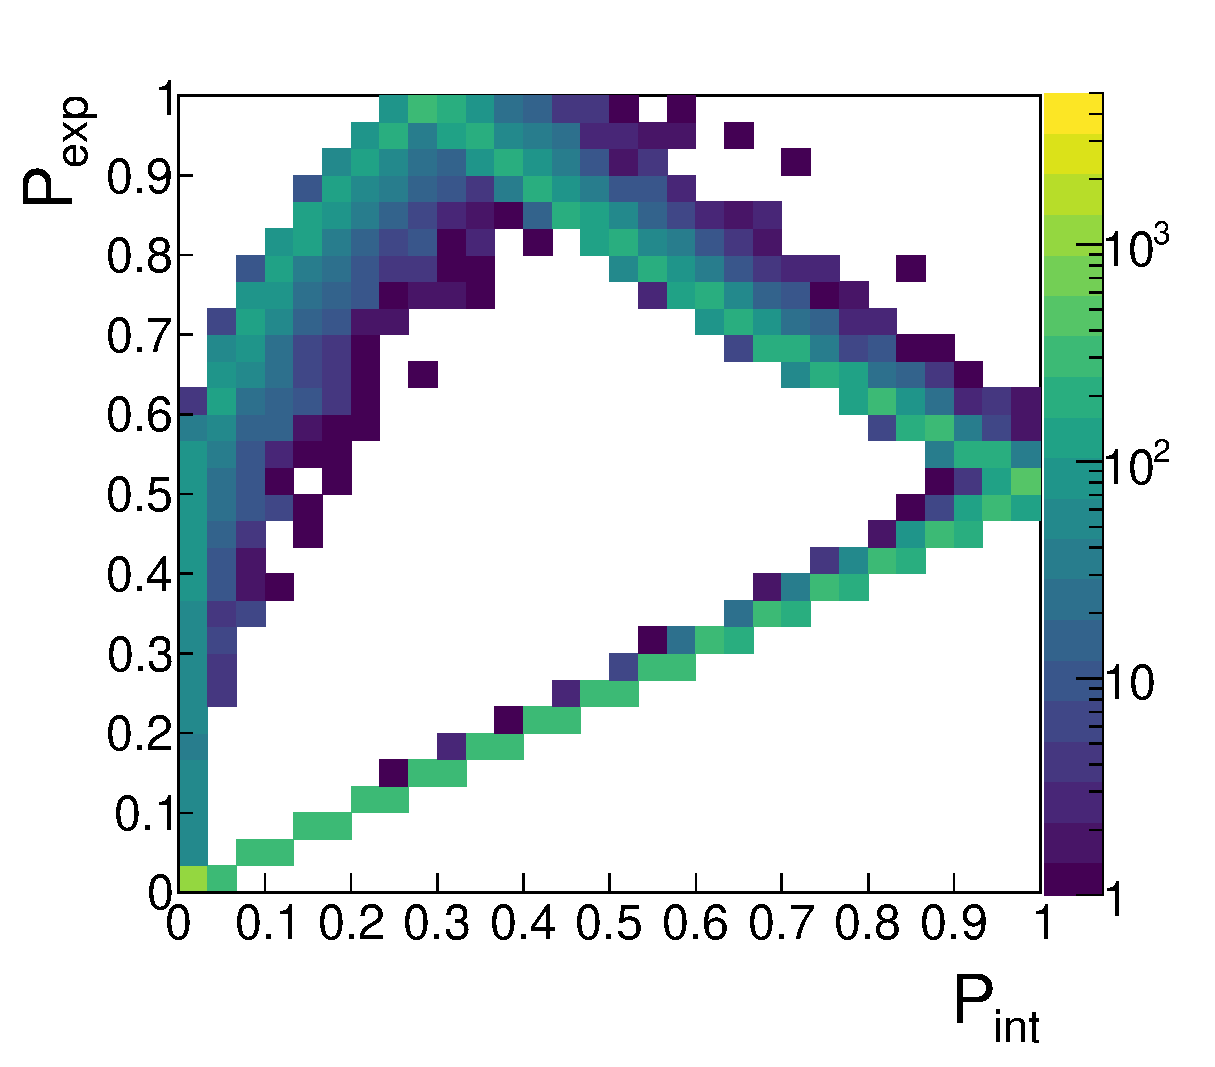
\includegraphics[width=0.76\textwidth]{timedifference/fig_timediff/PintVSPexp_0nubb_100.eps}
  \captionsetup{justification=justified}
  \caption{$\zeronu$ simulations, ${\sigma_{t}=100}$~ps.
    \label{subfig:}}
\end{subfigure}
%%\vskip\baselineskip
\begin{subfigure}[t]{0.49\textwidth}
  \centering
  \includegraphics[width=0.76\textwidth]{timedifference/fig_timediff/PintVSPexp_208Tl_300.eps}
  \captionsetup{justification=justified}
  \caption{\Tl simulations, ${\sigma_{t}=300}$~ps.
    \label{subfig:}}
\end{subfigure}
\hfill
\begin{subfigure}[t]{0.49\textwidth}
  \centering
  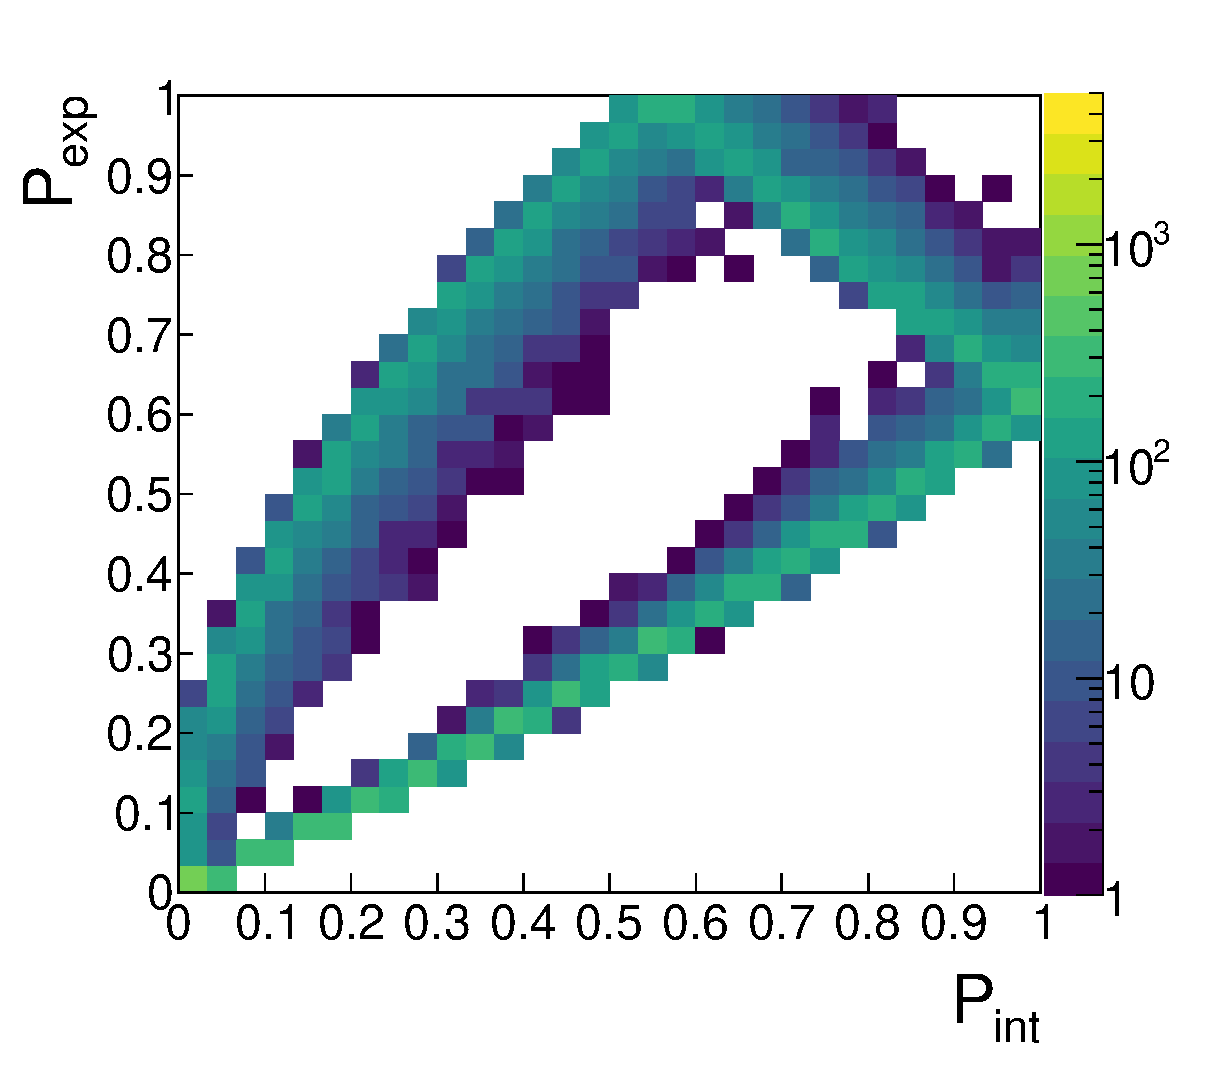
\includegraphics[width=0.76\textwidth]{timedifference/fig_timediff/PintVSPexp_0nubb_300.eps}
  \captionsetup{justification=justified}
  \caption{$\zeronu$ simulations, ${\sigma_{t}=300}$~ps.
    \label{subfig:}}
\end{subfigure}
%%\vskip\baselineskip
\begin{subfigure}[t]{0.49\textwidth}
  \centering
  \includegraphics[width=0.76\textwidth]{timedifference/fig_timediff/PintVSPexp_208Tl_400.eps}
  \captionsetup{justification=justified}
  \caption{\Tl simulations, ${\sigma_{t}=400}$~ps.
    \label{subfig:}}
\end{subfigure}
\hfill
\begin{subfigure}[t]{0.49\textwidth}
  \centering
  \includegraphics[width=0.76\textwidth]{timedifference/fig_timediff/PintVSPexp_0nubb_400.eps}
  \captionsetup{justification=justified}
  \caption{$\zeronu$ simulations, ${\sigma_{t}=400}$~ps.
    \label{subfig:}}
\end{subfigure}
\caption{\Pint$/P_{exp}$ biplots for different $\sigma_{t}$ values for \Tl\ and $\zeronu$ simulations.
  \label{fig:biplot_Pexp_Pint_sigma}}
\end{figure}
%%\end{changemargin}
Depending on $\sigma_{t}$, the area to be rejected moves towards higher values of \Pint.
Taking this into consideration, optimised values for \Pint\ have been set up, summarised in Tab.~\ref{tab:Pint_cutoff_sigma}.
\begin{table}[!h]
  \centering
  \begin{tabular}{|c|c|c|c|c|c|}
    \hline
    $\sigma_{t}$ (ps) & $0$ & $100$ & $200$ & $300$ & $400$ \\
    \hline\hline
    \Pint\ cut-off & [$0.05$ - $0.3$] & [0.25 - 0.6] & [0.4 - 0.7] & [0.5 - 0.8] & [0.55 - 0.85] \\
    \hline
  \end{tabular}
  \caption{Range of \Pint\ for which events are rejected.
    An additional cut-off with \Pint$<0.01$ and $P_{exp}<0.01$ is also applied.
    \label{tab:Pint_cutoff_sigma}}
\end{table}
To find an optimal value of $P_{exp}$ to be applied, several cut-offs are set up from $P_{exp}>0$ to $0.95$, and associated with the \Pint\ cut-offs presented in the previous table, in order to reject the required area.
Following the work done for the $\Delta t^{corr}$ cut-off, results are presented in Fig.~\ref{fig:eff_cut_proba_sigma} on an efficiency selection diagram.
\begin{figure}[!h]
  \centering
  \includegraphics[width=13cm]{timedifference/fig_timediff/compare_sigma_cut_proba.pdf}
  \caption{$\zeronu$ selection efficiency as a function of \Tl\ rejection.
    Each point corresponds to a minimal $P_{exp}$ value applied on the selected $2e$ topologies.
    \Pint\ selections are also applied, their value depending on the $\sigma_{t}$ value (Tab.~\ref{tab:Pint_cutoff_sigma}).
    $\sigma_{l}=27.8$~ps.
    \label{fig:eff_cut_proba_sigma}}
\end{figure}
The calorimeter timing measurement has a great influence, especially on \Tl\ events rejection.
Evolution of selection efficiencies for ${\sigma_{t}<200}$~ps are very similar, reaching a plateau for ${\sim P_{exp}>0.25}$ allowing to reject $20$\% of \Tl\ while keeping $85$\% of $\zeronu$.
Below $\sigma=100$~ps the background rejection is improved despite a loss in signal selection efficiency, up to reaching $\sim45$\% of \Tl\ rejection and $\sim80$\% signal selection for an ideal calorimeter.
The plateau is reached at $P_{exp}>0.2$ for $\sigma_{t}=100$~ps and $P_{exp}>0.15$ for $\sigma_{t}=0$~ps.

A better Thallium rejection can be obtained with the simple selection on time-of-flights, but the probability one has the main advantage to be more accurate as it takes into account the calorimeter time measurement uncertainties.
Moreover, even if variations of selection/rejection of this diagram are not as pronounced as for the $\Delta t^{corr}$ cut-off, a strong assumption can be made: the more we are precise on time-of-flight measurements, the more we are able to reject \Tl\ events while keeping a satisfying part of signal.
During the calorimeter R\&D, a great effort has been made to improve the optical modules energy resolution compared to NEMO-$3$, notably because it allows to have a better background rejection, and thus to decrease its contribution to the $\zeronu$ search.
Finally, in view of these results, a good timing precision in calorimeter blocks is also important when it concerns background rejection, and especially the identification of $\beta$+IC delayed \Tl\ decays.
Nevertheless, to give a final conclusion on the usefulness of the $\Delta t^{corr}$ and probability cut-offs, one have to study its impact on the final sensitivity of the detector, which is dealt with in the next section.

%% \begin{figure}[!h]
%%   \centering
%%   \includegraphics[width=13cm]{timedifference/fig_timediff/efficiency_proba.pdf}
%%   \caption{$\zeronu$ selection efficiency as a function of \Tl\ rejection.
%%     Each data point corresponds to a given value of $\sigma_{t}$, decrementing in $50$~ps steps.
%%     First order selections applied on $\zeronu$ and \Tl\ simulations.
%%     $\sigma_{l}=27.8$~ps.
%%     \label{fig:eff_proba_sigma}}
%% \end{figure}


\section{Impact of \Tl\ rejection on the experiment's sensitivity}
\label{sec:Tl_sensitivity}

In the previous sub-section were presented results for $\Delta t^{corr}$ and optimised probability cut-offs, and the influence of the calorimeter time resolution on these rejection techniques was reviewed.
Nevertheless, to properly quantify the effectiveness of these cut-off, one have to study their impact on the final detector sensitivity ($500$~kg.y exposure).
To do so, the procedure described in Chapter~\ref{ch:sensitivity} is applied to the $2e$ topologies selected (after the application of $\Delta t^{corr}$ or probability cut-offs), for signal and backgrounds considered ($\twonu$, \Bi, \Tl\ and \Rn).

\subsection{Sensitivity results}

The variations of the sensitivity are presented in Fig.~\ref{fig:T12_cut} for three values of $\sigma_{t}$ at $1$~MeV, as a function of the cut-off levels applied.
\begin{figure}[!h]
\centering
\begin{subfigure}[t]{1\textwidth}
  \centering
  \includegraphics[width=0.98\textwidth]{timedifference/fig_timediff/compare_sigma_cut_delta_t_T12.pdf}
  \captionsetup{justification=justified}
  \caption{$\Delta t^{corr}$ cut-off.
    \label{subfig:T12_cut_deltat}}
\end{subfigure}
\begin{subfigure}[t]{1\textwidth}
  \centering
  \includegraphics[width=0.98\textwidth]{timedifference/fig_timediff/compare_sigma_cut_proba_T12.pdf}
  \captionsetup{justification=justified}
  \caption{Probability cut-off.
    \label{subfig:T12_cut_proba}}
\end{subfigure}
\caption{(Top pad) $\Tbeta$ at $90$\% CL and (bottom pad) optimised ROI, as a function of the minimal value of $\Delta t$ applied on the selected $2e$ topologies.
    Results are given for $\sigma_{t}=0$, $200$ and $400$~ps at $1$~MeV, and $\sigma_{l}=27.8$~ps.
  \label{fig:T12_cut}}
\end{figure}
For these two figures, the more the $x$-values increase, the more the applied cut is released.
In both cases sensitivity results converge towards $\sim2.4\times10^{25}$~years, for very loose values of the selection.
%% This value is slightly different than the final results given in Chapter~\ref{ch:sensitivity}, due to the energy cut-off which is firstly applied on $2e$ topologies in the current study (Sec.~\ref{subsec:energy_seletion}).

Regarding the influence of $\Delta t^{corr}$ selection, a sensitivity improvement can eventually be obtained by applying this selection, depending on the value of $\sigma_{t}$ considered for the calorimeter (Fig.~\ref{subfig:T12_cut_deltat}).
\begin{itemize}
\item $\sigma_{t}=0$~ps at $1$~MeV: an improvement of $12$\% on the sensitivity is observed for events rejected if $\Delta t^{corr}>200$~ps.
  This is consistent with the \Pb\ metastable level of $294$~ps to which we are very sensitive with such ideal value of the calorimeter resolution.
\item $\sigma_{t}=200$~ps at $1$~MeV: a slighter improvement of $6$\% is reached for $\Delta t^{corr}>550$~ps.
  As the calorimeter time resolution is reduced, compared with the first ideal case, a smaller improvement can be obtained, for a loose value of the applied cut.
\item $\sigma_{t}=400$~ps at $1$~MeV: the resolution is too degraded for an improvement to be obtained with such a time-of-flight cut-off.
\end{itemize}

Concerning the influence of probability selection, values of $\Tbeta$ also converge towards a unique value, attained for $P_{exp}>1$, meaning all the events are selected for such a level.
In other words, the more restrictive this cut is, the more the sensitivity is reduced.
The least unfavourable case is obtained for the ideal calorimeter resolution case, with stagnation of the values on a plateau, for most of the applied cut-off levels.
Even if it is less wide, a plateau is also reached for $\sigma_{t}=200$~ps.


\subsection{Expected number of background}

The influence of the $\Delta t^{corr}$ selection on the number of expected background events in the optimised ROI is presented in Tab.~\ref{tab:Nbkg_deltat_cut}.
\begin{table}[h!]
  \centering
  \begin{tabular}{|c|c|c|c|}
    \hline
    $\sigma_{t}$ (ps) & $0$ & $200$ & $400$ \\
    ROI (MeV) & [$2.7$;$2.95$] & [$2.7$;$2.9$] & [$2.7$;$2.95$] \\
    Minimal $\Delta t^{corr}$ (ps) & $200$ & $550$ & $650$ \\
    $\Tbeta$ ($90$\% CL) ($\times10^{25}$~y) & $2.7$ & $2.5$ & $2.4$ \\
    $\mbb$ ($90$\% CL) (eV) & $[0.11-0.22]$ & $[0.11-0.22]$ & $[0.12-0.23]$ \\
    \hline\hline
    $\epsilon_{0\nu}$ & $14.6$\% & $14.2$\% & $12.9$\% \\
    \hdashline
    $\twonu$  & $10.8$ & $10.8$ & $9.58$ \\
    \Tl  & $9.52$ & $13.3$ & $13.4$ \\
    \Bi  & $42.9$ & $42.0$ & $39.2$ \\
    \Rn  & $1.12$ & $1.12$ & $1.04$ \\
    Total & $64.4$ & $67.2$ & $63.2$ \\
    \hline
  \end{tabular}
  \caption{Expected number of background events in the optimised ROI, for the exposure of the SuperNEMO final detector ($500$~kg.y).
    Three values of $\sigma_{t}$ are considered for which the best $\Delta t^{corr}$ is applied.
    \label{tab:Nbkg_deltat_cut}}
\end{table}
Three values of $\sigma_{t}$ are considered, and for each of them the best level for this cut, determined in the previous sub-section, is applied.
The best rejection of Thallium is reached for the ideal calorimeter time resolution, as the two electrons time-of-flights are measured precisely.
For $\sigma_{t}=200$~ps, a smaller amount of Thallium background is rejected, but the $\zeronu$ selection efficiency remains stable.
This selection efficiency is affected when the time resolution is degraded to $\sigma_{t}$, thus when the delayed events are badly discriminated compared with the simultaneous ones.
As expected, other background events ($\twonu$, \Bi\ and \Rn) are not significantly affected by this selection.

As discussed, the probability cut-offs applied on $2e$ topologies only degrade the final sensitivity to the $\zeronu$ process.
To quantify its impact on the background rejection, we present in Tab.~\ref{tab:Nbkg_proba_cut} the expected number of background in the optimised ROI, for two different levels for the $P_{exp}$ selection, one at $0.5$ and the other one very loose.
\begin{table}[h!]
  \centering
  \begin{tabular}{|c|c|c|}
    \hline
    ROI (MeV) & [$2.7$;$2.9$] & [$2.7$;$2.9$] \\
    Minimal $P_{exp}$ & $0.5$ & $0.95$ \\
    $\Tbeta$ ($90$\% CL) ($\times10^{25}$~y) & $2.2$ & $2.4$ \\
    $\mbb$ ($90$\% CL) (eV) & $[0.12-0.24]$ & $[0.12-0.23]$ \\
    \hline\hline
    $\epsilon_{0\nu}$ & $12.1$\% & $13.9$\% \\
    \hdashline
    $\twonu$  & $9.83$ & $10.8$ \\
    \Tl  & $16.3$ & $21.0$ \\
    \Bi  & $38.4$ & $42.0$ \\
    \Rn  & $0.596$ & $0.596$ \\
    Total & $65.1$ & $74.4$ \\
    \hline
  \end{tabular}
  \caption{Expected number of background events in the optimised ROI, for the exposure of the SuperNEMO final detector ($500$~kg.y).
    The time resolution is taken as $\sigma_{t}=200$~ps.
    Two levels of $P_{exp}$ cut are compared, $0.5$ and $0.95$.
    \label{tab:Nbkg_proba_cut}}
\end{table}
Even if it affect the $\zeronu$ selection efficiency, this selection allows to reject $5$ events of \Tl\ inside the ROI for the SuperNEMO final detector.

These two selections were implemented in order to reject \Tl\ events and they have fulfilled this role.
The $\Delta t^{corr}$ selection allowed to improve the sensitivity by $12$\% for a perfect calorimeter time resolution.
Finally, the final detector sensitivity is greatly affected by this timing measurement precision.



\section{Conclusion}

During this chapter we have defined or specified analysis tools adapted to the rejection of background.
In particular, a so-called exponential probability law has been defined to describe the internal events of delayed Thallium.
Although the cut-off based on the electron time-of-flight is very satisfactory for rejecting this last background, the associated cut-off in internal and exponential probability makes it possible to be more precise since it takes into account the errors made on the time-of-flight measurements in the calorimeter.
These rejection could be tested on site using a $^{232}$U calibration source, a parent of \Tl\ nucleus, inside the calorimeter to check the \Tl\ rejection using time-of-flight.

We have determined the influence the time resolution has on the various defined cut-off efficiencies.
The worse this resolution is, the more difficult it is to discriminate thallium events from signal events.
Improving the time resolution of the calorimeter was not a direct purpose of the R\&D programme, however it has benefited from the high light output achieved to meet the energy resolution goals.
The time resolution of the optical modules has been monitored at every stage of the R\&D programme but remains to be precisely determined.
This is precisely the purpose of the next chapter, which describes how we determined the time resolution of the optical modules of the demonstrator calorimeter with a \Co\ source.

               \chapter{Characterisation of the calorimeter time resolution}
\label{ch:Cobalt_study}

The precise knowledge of the different particle interaction times in the optical modules of the SuperNEMO calorimeter is important to better understand and reject the background.
For example, the study of electron time-of-flight allows us to distinguish internal events (occurring within the source foils) from external events (radioactive decays occurring outside the source foils, for example in the PMTs or in the iron shielding).

During the commissioning phase, a lot of work, presented in the previous chapter, was achieved to calibrate the detector.
Following on from this task and completing it, a great part of my PhD was allocated to determine the time resolution of the SuperNEMO calorimeter, and to provide tools to the collaboration to purchase this analysis.

In this chapter we present different studies conducted in order to characterise the time response of the SuperNEMO optical modules.
Although the goal of the presented studies is to characterise the time resolution of the SuperNEMO calorimeter, some detector adjustments were still ongoing at the time of the acquisition, that could influence the presented results.
Especially, the energy calibration described in Sec.~\ref{sec:comm_energy_calibration} was not complete, and the Light Injection System presented in Sec.~\ref{sec:LIS} was not yet fully operational.
However, all the work presented here is necessary in the framework of the first calorimeter calibration.
Moreover, I provide all the analysis tools for the collaboration, with a view to doing a possible update, once the whole demonstrator calibration will be achieved.

The first study presented in this chapter focuses on the characterisation of the time resolution of the SuperNEMO calorimeter, using a calibration source made of \Co.
In the second part of this chapter, we study the possibility to gather informations on the calorimeter time resolution using the Light Injection System, a set-up initially designed to calibrate in energy the calorimeter.

%%%%%%%%%%%%%%%%%%%%%%%%%%%%%%%%%%%%%%%%%%%%%%%%%%%%%%%%%%%%%%%%%%%%%%%%%%%%%%%%%%%%%%%%%%%%%%%%%%%%%%%%%%%%%%%%%%%%%%%%%%%%%%%%
\section{Interaction of particles in the SuperNEMO scintillators}
\label{sec:scintillator_interactions}

Understanding how particles interact in the SuperNEMO scintillators is essential.
The calorimeter part of the demonstrator mainly aims to detect electrons and photons.
In this section, we review ***.


\subsection{Interaction of electrons}

Electrons interact with matter through one of two processes: elastic scattering on a nucleus, or inelastic scattering on an atomic electron.
Inelastic scatterings are dominant for polystyrene scintillators and occur through two different forms: coherent scattering with the electron cloud, and radiative energy losses (the so-called bremsstrahlung effect).
In Fig.~\ref{subfig:electron_attenuation} is displayed the stopping power of electrons in polystyrene for these two processes.
\begin{figure}[h]
  \centering
  \begin{subfigure}[t]{0.48\textwidth}
    \centering
    \includegraphics[width=1\textwidth]{commissioning/fig_commissioning/electron_energy_loss.pdf}
    \captionsetup{justification=centering}
    \caption{
      \label{subfig:electron_attenuation}}
  \end{subfigure}
  \hfill
  \begin{subfigure}[t]{0.48\textwidth}
    \centering
    \includegraphics[width=1\textwidth]{commissioning/fig_commissioning/free_path_electrons.pdf}
    \captionsetup{justification=centering}
    \caption{\label{subfig:electron_free_path}}
  \end{subfigure}
  \caption{Stopping power (a) and mean free path (b) for electrons in polystyrene.
    (a) Energy losses through radiative effect (orange dashed line) and coherent scattering (red dashed line), which is the dominant process for the considered energy range~\cite{web:nist_estar}.
    %  operate mainly through coherent scattering.
    (b) At $1$ MeV, the mean free path of an electron is about $3$ mm.
    Adapted from~\cite{HuberThesis}.
  }
\end{figure}
Electrons detected in the SuperNEMO calorimeter should deposit a minimal energy of $50$ keV (the acquisition low energy threshold) and a maximal energy of few MeV (depending on the $\twonu$ isotope).
In this energy range, collisions with the electron cloud are preponderant compared with radiative energy losses.
In Fig.~\ref{subfig:electron_free_path}, we give informations about the mean free path of an electron in polystyrene.
In particular, we observe that an electron of $1$ MeV penetrates, on average, several millimetres into a polystyrene scintillator.


\subsection{Interaction of photons}

Photons travelling in  matter can interact with the electronic cloud, through three main processes, whose contributions are presented in fig.~\ref{subfig:photon_energy_loss}, depending on their energies.
\begin{figure}[h]
  \centering
  \begin{subfigure}[t]{0.48\textwidth}
    \centering
    \includegraphics[width=1\textwidth]{commissioning/fig_commissioning/photon_energy_loss.pdf}
    \captionsetup{justification=centering}
    \caption{\label{subfig:photon_energy_loss}}
  \end{subfigure}
  \hfill
  \begin{subfigure}[t]{0.48\textwidth}
    \centering
    \includegraphics[width=1\textwidth]{commissioning/fig_commissioning/attenuation_length_photons.pdf}
    \captionsetup{justification=centering}
    \caption{\label{subfig:attenuation_length_photons}}
  \end{subfigure}
  \caption{Linear attenuation coefficient (a) and attenuation length (b) for $\gamma$ radiations in a plastic scintillator made of polystyrene.
    (a) In the considered energy range of $10$ keV $ -\; 10$ MeV, $\gamma$ radiations interact with matter mainly through Compton diffusion~\cite{web:nist_Xcom}.
    (b) The attenuation length of a $\gamma$ radiation is about $10$ cm at $1$ MeV.
    Adapted from~\cite{HuberThesis}.
  }
\end{figure}
Low-energy photons mainly interact with the electron cloud, either through photoelectric effect ($\gamma$ radiation is fully absorbed by an electron of the cloud), or through coherent (so-called Rayleigh) scattering.
But the dominant effect, for energies between $10$ keV and $10$ MeV, is the Compton inelastic scattering of a $\gamma$ with an atomic electron.
In Fig.~\ref{subfig:attenuation_length_photons}, we display the mean attenuation length of a $\gamma$ radiation in polystyrene scintillators, with energy.
Thus, most of $1$ MeV $\gamma$ radiations will interact around $10$ cm inside the scintillating material.

At the considered energy range ($10$ keV $ -\; 10$ MeV), the interaction of photons with matter is dominated by Compton effect, while the electrons interact mainly through coherent scattering.
The SuperNEMO scintillators are designed to detect such particles.
Photons have a high probability to interact inside the volume of the scintillator, while electrons are stopped in the first few millimetres.

The following section are devoted to the study of the time resolution of the SuperNEMO optical modules.



%%%%%%%%%%%%%%%%%%%%%%%%%%%%%%%%%%%%%%%%%%%%%%%%%%%%%%%%%%%%%%%%%%%%%%%%%%%%%%%%%%%%%%%%%%%%%%%%%%%%%%%%%%%%%%%%%%%%%%%%%%%%%%%%
\section{Measurement of the time resolution with a $^{60}$Co source}
\label{sec:Co_analysis}
This section is dedicated to detail the time resolution study performed using a \Co\ source, exploiting the time characteristic of two photons emitted during the radioactive disintegration process of this nucleus.
A great proportion of the whole SuperNEMO demonstrator was successfully characterised using this radioactive source.

\subsection{Time response of optical modules}
\label{subsec:OMtimeResponse}

In order to characterise the energy and time-of-flight of incoming particles (photons, electrons), each calorimeter block of SuperNEMO is composed of a scintillator and a photomultiplier.
As detailed in Chapter~\ref{ch:detector}, the purpose of the scintillator material is to stop the incoming particles, which will induce the production of the so-called optical photons.
The optical photons reaching the photomultiplier photocathode are then converted into electrons, with an efficiency called quantum efficiency.
After amplification, electrons are collected by the anode which delivers an electric signal whose charge proportional to the initial amount of incident photoelectrons.
This signal is then transmitted, via the PM voltage divider, to the electronic readout, where the signal is sampled.
The particle energy, as well as the time-of-flight, can be extracted from the signal waveform analysis.
Each step of the particle detection process, from the incident particle interaction inside the scintillator, to the signal sampling at the electronic readout, can have an impact on the precise time measurement of the charged particle.
In Chapter~\ref{ch:detector} and \ref{ch:timediff} we introduced the so-called calorimeter time resolution $\sigma_t$, which encapsulates the global uncertainty on the time-of-flight measurement of particles into the calorimeter (Eq.~\eqref{eq:sigma_t}).
The squared time-resolution can therefore be expressed as the sum of two contributions:
the scintillator resolution $\sigma_{t, \textrm{sc}}^{2}$, and the PMT resolution $\sigma_{t, \textrm{PM}}^{2}$,
\begin{equation}
  \sigma_{t}^{2}=\sigma_{t,\text{sc}}^{2}+\sigma_{t,\text{PM}}^{2}\,.
  \label{eq:Co_sigma_t}
\end{equation}
In the following, we detail in depth the physical origins of these terms.

\subsubsection*{Scintillator time dispersion}
The scintillator temporal dispersion $\sigma_{t,\text{sc}}$ in Eq.~\eqref{eq:Co_sigma_t} receives contributions mainly from two important characteristics of the scintillator operating principle.

\paragraph{Interaction point:}
The incoming particle's interaction point location inside the scintillator block highly contributes to the scintillator temporal uncertainty, and depends on the incident particle type.
In fact, this effect will not have the same impact on time dispersion, depending on whether the incident particle is a photon or an electron.
In Fig~\ref{fig:photon_scintilator} are schemed the interactions of a photon and that of an electron for the specific case of a SuperNEMO plastic scintillator.
\begin{figure}[h]
  \centering
  \includegraphics[width=8cm]{commissioning/fig_commissioning/Co_multi_reflection.pdf}
  \caption{A scheme of interaction of particles in a scintillator.
    The photon case is displayed on the left in pink dotted line, and the electron case is on the right in dark blue dotted line.
    Both particles enter in the scintillator through the front face.
    Examples of interaction points inside the scintillator are represented by the black dots.
    The photons of scintillation emitted isotropically after the interaction are materialised by the bright green dotted lines.
    Due to different interaction probabilities in matter, the two particles intercat at different depths inside the scintillator.
    The photon can interact deeply inside the volume, while the electron has a high probability to stop within the first few millimetres.
    \label{fig:photon_scintilator}}
\end{figure}
In Sec.~\ref{sec:scintillator_interactions}, we exposed the different interaction types of photons and electrons.
We have also explained the origin of the differences that exist in terms of interaction depth between these two types of particles.
To remain consistent with these conclusions, we represent the electron as interacting in the first millimetres, while the photon stops deep inside the scintillator.
When a particle (photon or electron) interacts in the scintillating material, the absorbed energy leads to the isotropic emission of scintillation photons:
they propagate inside the scintillator, in all directions from the interaction point, at the speed of $c/n_{sc}$, with $n_{sc}$ the optical index of polystyrene, and $c$ the light speed in vacuum.
Depending on their initial direction, some of those photons propagate straight to the PMT (we name them the \emph{direct} photons), while others are at least reflected once on the scintillator surface, before reaching the PM glass.
This mechanism leads to time delays between direct and reflected photons.

In order to illustrate, and give an order of magnitude of this delay, let us consider an example where an incoming electromagnetic particle enters a scintillator from the front face, and interacts right in the centre of the scintillator volume.
After the scintillation emission process, a direct photon will reach the PM glass surface at time
\begin{equation}
  t_{s} = \frac{L}{2c/n_{sc}}\,,
\end{equation}
$L$ being the scintillator width.
Now, let us consider another photon, that we name \emph{backward reflected}, emitted in the opposite direction.
It will propagate, reflect on the front scintillator surface, and finally reach the PM at
\begin{equation}
  t_{r} = \frac{3L}{2c/n_{sc}}\,.
\end{equation}
This reflected photon is therefore delayed compared to the direct photon, with a time-shift of
\begin{equation}
  \Delta t^{r,s} = t_{r} - t_{s} = \frac{L}{c/n_{sc}}\,.
\end{equation}
In the case of a SuperNEMO scintillator, the length $L$ has been designed to $25$ cm, and the optical index is the one of polystyrene with $n_{sc}=1.5$.
Finally, for an incoming particle interacting at the centre of a SuperNEMO scintillator volume, a backward reflected scintillation photon will reach the PM glass $1.25$ ns later than a direct photon.
And this delay is even more important as the incident particle interacts deep inside the scintillator.

In view of the conclusions given in Sec.~\ref{sec:scintillator_interactions}, we know that photons have a higher probability of interacting far into the scintillator block, compared with electrons.
Therefore, this time-shift effect is all the more important for incoming photons, while it is quite negligible for incoming electrons, for which reflected photoelectrons reach the PM glass almost as the same time as the direct ones.

This mechanism increases the signal collection rising time at the PM anode, and boosts the scintillator time dispersion $\sigma_{t,\text{sc}}$, with $\sigma_{t,\text{sc}}^{\gamma}>\sigma_{t,\text{sc}}^{\text{e}^{-}}$.

\paragraph{Scintillating light emission:}
When a particle interacts in a SuperNEMO scintillator, two successive mechanisms of light absorption/re-emission take place.
Firstly, the excitation of scintillator molecules leads to the creation of fluorescence photons.
Afterwards, those optical photons are absorbed, then re-emitted by the POPOP agent, at higher wavelengths.
The characteristic times of these two processes contribute to increase the scintillator time dispersion $\sigma_{t,\text{sc}}$.
%% These two processes follow the same temporal distribution
%% \begin{equation}
%%   \mathcal{N}_{\text{photons}} = A\times e^{-t/\tau}\,,
%%   \label{eq:fluorescence_photons_time}
%% \end{equation}
%% with $\mathcal{N}_{\text{photons}}$ the number of generated photons at time $t$, $A$ a normalisation constant and $\tau$ the fluorescence characteristic time of the considered process.

\subsubsection*{Photomultiplier time dispersion}

A photomultiplier is a photodetector: after the light is collected and converted at the photocathode, the photoelectrons are multiplied.
The transit time for the photoelectrons emitted at the photocathode to reach the anode after being multiplied is not constant for every photoelectron, due to a varying path for electrons emitted by the different dynodes.
This results in a timing dispersion.
This fluctuation is called transit time spread (TTS).
It leads to an uncertainty on the time measurement and so has an influence on the photomultiplier time dispersion $\sigma_{t,\text{PM}}$.

As discussed in Chapter~\ref{ch:timediff}, the time uncertainty brought by the scintillator light emission process and the photomultiplier was characterised for each optical module before the calorimeter assembly.
It is possible that the optical modules time resolutions may have changed during the phases following their measurement, so they must be measured again.
To do so, data acquisitions were taken with the calorimeter, behind which a \Co\ calibration source was set, allowing to detect the two emitted $\gamma$'s.


\subsection{Description of \Co\ nucleus}
\label{subsec:CoSource}
The \Co\ is a man-made isotope, with a $5.27$ years half-life, of which we provide the main interesting properties in the simplified decay scheme of Fig.~\ref{fig:Co_decay_scheme}.
\begin{figure}[h]
  \centering
  \includegraphics[width=9cm]{commissioning/fig_commissioning/Co_decay_scheme.pdf}
  \caption{A simplified decay scheme for \Co~\cite{web:nucleide}.
    The Cobalt decays, through $\beta^{-}$, predominantly to the $2.50$ MeV state.
    Then, two succesive $\gamma$'s (whose energy levels are represented in green) are emitted in $99.83$\% of the cases.
    The two photons have an energy of $1.17$ MeV and $1.33$ MeV, respectively.
    As the life-time of the $1.33$ MeV energy level is short ($<1$ ps) with respect to the timing precision of the calorimeter, the two photons can be considered as emitted in coincidence.
    We use this property to calibrate in time the demonstrator optical modules.
    \label{fig:Co_decay_scheme}}
\end{figure}
This unstable nucleus spontaneously decays, through the $\beta^{-}$ process, into an excited state of Nickel $60$.
To reach the ground state of the Nickel $60$, the nucleus goes through two successive energy levels, emitting in $99.83$\% of the cases two photons of $1.17$ MeV and $1.33$ MeV, respectively.
The life-time of the second energy level is under the picosecond, thus very short with respect to the expected timing precision of the calorimeter.
Therefore, the two photons are considered as emitted in coincidence.

We aim to detected these two photons and look for coincidences between pairs of optical modules to determine their time resolution.


\subsection{Experimental design}
\label{subsec:Co_setup}


The idea to use a \Co\ source to characterise the time response of the calorimeter part of SuperNEMO had never been tested before the current analysis.
Therefore, all the experimental design had to be implemented.


\subsubsection*{Setting up the experimental design}


The initial activity of the Cobalt source we used for this experimental set-up was $447.4$ kBq in February $2014$.
Given the half-life of this isotope, it was reduced to $232$ kBq at the time of the data-taking.
In order to determine the best design, and later to monitor and compare the results obtained in the framework of this analysis, I performed simulations of \Co\ disintegrations for the demonstrator configuration.
The characteristics of those simulations are detailed later in this section.

As described in Chapter~\ref{ch:detector}, the SuperNEMO calorimeter is composed of two main walls (called \emph{French} and \emph{Italian} sides), as well as the so-called X-Walls (on the detector sides) and $\gamma$-Vetos (on top and below the detector).
At the time of the data-taking, X-Walls and $\gamma$-Vetos were not yet operational, hence the current analysis only applies on the French and Italian main calorimeter walls.
As the demonstrator was closed at this time, it was impossible to set the Cobalt source inside the detector, at the source foils level.
Hence, the calibration source was placed behind the calorimeter, as displayed in Fig.~\ref{fig:Co_exp_design}, where sketches of side and back views of the calorimeter are drawn.
\begin{figure}[h]
  \centering
  \begin{subfigure}[t]{0.48\textwidth}
    \centering
    \includegraphics[height=0.5\textwidth]{commissioning/fig_commissioning/Co_setup.pdf}
    \captionsetup{justification=justified}
    \caption{
      \label{subfig:Co_setup}}
  \end{subfigure}
  \hfill
  \begin{subfigure}[t]{0.48\textwidth}
    \centering
    \includegraphics[height=0.5\textwidth]{commissioning/fig_commissioning/Co_setup_wall.pdf}
    \captionsetup{justification=justified}
    \caption{
      \label{subfig:Co_setup_wall}}
  \end{subfigure}
  \caption{(a) Side view example of the Cobalt source positioning behind a calorimeter main wall, schemed by $4$ optical modules (green).
    The emissions of the $2$ $\gamma$'s of interest are displayed in coloured dotted lines.
    (b) Back view of the nine source positions behind a main wall.
    Each grey box represents an optical module.
    \label{fig:Co_exp_design}
  }
\end{figure}
In order for all PMs to detect $\gamma$'s from Cobalt decays, several bunches of data acquisitions were taken:
the source was placed at $9$ different positions on each of the $2$ main calorimeter walls, approximately one meter behind.
Therefore, in total, $19$ data acquisitions have been taken, of which:
\begin{itemize}
\item $18$ with the Cobalt source set behind the wall. The $9$ different positions for one wall are represented in Fig.~\ref{subfig:Co_setup_wall}.
\item $1$ acquisition have been taken without the Cobalt source, with the Italian main wall, to characterise the background detected with the current calorimeter settings.
\end{itemize}
Each data acquisition lasted about $25$ minutes, for a total of $10$ hours of on-site activities, taking into account the time needed to move the Cobalt source from spot to spot.

Currently, the demonstrator is not protected from the laboratory lights by the anti-radon tent.
As laboratory lights would damage the SuperNEMO photomultipliers under tension, two removable black curtains are deployed on top of the detector (that do not interfere with data collection), and acquisitions are taken in dark laboratory.
With this way of doing, all data acquisitions can be performed, while eventual necessary repairs remain possible during the detector commissioning.

Taking acquisitions in the dark is a big constraint.
Moreover, the Cobalt source, initially used for teaching purposes, was loan by IPN laboratory (Orsay), for only two weeks, mainly because of legal constraints.
Therefore, to not disturb LSM on-site activities by plunging the whole laboratory into darkness, and to make the loan time profitable, a SuperNEMO team and I performed night shifts to take data.
The acquisition took place during two weeks, at the summer break $2019$.

\subsubsection*{Simulations and analysis pipelines}


As for the data acquisition, the simulated source has been placed behind the calorimeter walls.
Hopefully, there was no need to simulate all the $18$ positions.
In fact, at this time, the detector implemented in simulations is symmetrical in terms of detection performances.
Therefore, simulations of \Co\ events behind the two main walls are equivalent, and we only need to simulate events from $4$ locations (positions $1$, $2$, $4$ and $5$, according to the Fig.~\ref{subfig:Co_setup_wall} numbering system), other being obtained by symmetry operations.
Four bunches, for a total of $10^{9}$ Cobalt events, were simulated with the official Falaise pipeline and stored at the IN$2$P$3$ computing centre platform, making them available to the collaboration.

As the objective is to determine the optical modules time resolution, $\sigma_{t}$, due to the scintillator light emission process and to the photomultiplier, all simulations were performed with an ideal calorimeter, setting up ${\sigma_{t}=0}$~ps.
In that case, the only remaining contribution of optical modules to the time resolution is geometrical and comes from the interaction point uncertainty inside the scintillator.
The idea behind that is to compare simulated and real data in order to bring out the contribution of $\sigma_{t}$ to the total calorimeter time uncertainty.

%% A visualisation, provided by the Falaise Software, of a simulated Cobalt event behind the Italian calorimeter main wall, is shown in Fig.~\ref{fig:Co_visu}.
%% \begin{figure}[h]
%%   \centering
%%   \includegraphics[width=6cm]{commissioning/fig_commissioning/Co_visu.pdf}
%%   \caption{Visualisation of a simulated Cobalt event.
%%     \label{fig:Co_visu}}
%% \end{figure}

%% \paragraph{Background events simulations:}
%% As already discussed in Chapter~\ref{ch:sensitivity}, currently the collaboration does not supply a complete set of external background simulations for the demonstrator design.
%% This will be implemented as soon as the final demonstrator performances has been determined.
%% Thus, we did not have at our disposal background events simulations for this analysis.

The entire experimental set-up was designed and carried out by me and a group of physicists from LAL, Orsay and LPC, Caen.
I developed a complete set of ROOT codes for data processing and analysis, available on the GitHub platform~\cite{myGit}.
As the tracker is not yet operational for data collection at Modane, we are only interested in the part of the simulations with the calorimeter.
The PID module was therefore not used in the reconstruction pipeline, and other criteria, described in the following sub-section, were used to select the Cobalt events of interest.
A single off-line analysis pipeline has been developed to handle the different output data models of the simulations and real data, in order to ensure the consistency of the analysis.

\subsection{Signal events selection}
\label{subsec:Co_datacut}

We aim to use the two $\gamma$'s of $1.17$ MeV and $1.33$ MeV from \Co\ $\beta^{-}$ decay, to characterise the time resolutions of individual optical modules.
Thus, the signal we are looking for is two particles detected in coincidence in distinct optical modules.
In order to maximise the signal to background ratio, some selections have been applied on data.
\begin{itemize}
\item Trigger criteria:\\ in the two calorimeter hits channel, the trigger condition is defined so as one of the two hit has to trigger the low energy (or amplitude) threshold, of $50$~keV for the data acquisition.
  As we look for two calorimeter hits, we set an additional off-line selection events whose two hits passed both the high amplitude threshold, corresponding to approximately $150$ keV.
\item Coincidence time criterion:\\ we define the coincidence time-window by events occurring in a $62.5$ ns-long time interval.
  This allows to avoid accidental coincidence events (interactions of two gammas, produced by different sources, in two optical modules), while keeping events where two $\gamma$ particles interact at both ends of the wall.
  This time-window was set for the data-taking and can be improved for eventual future acquisitions.
\item Individual energy selection:\\ in Fig.~\ref{fig:Co_energy_cut} is displayed the highest energy deposit as a function of the lowest energy deposit, for simulations with the \Co\ source in position $5$.
  \begin{figure}[h]
    \centering
    \includegraphics[width=14cm]{commissioning/fig_commissioning/Co_energy_cut.pdf}
    \caption{Maximal energy with minimal energy, for simulated \Co\ events, with source in position $5$ (see Fig.~\ref{subfig:Co_setup_wall}).
      High threshold is represented in black dotted line.
      Dashed lines materialise the individual energy selection.
      \label{fig:Co_energy_cut}}
  \end{figure}
  The high energy threshold is represented by two black dotted lines.
  The topology of interest is observable with two hits around $1$~MeV.
  Also, events where two successive Compton interactions of a single photon from Cobalt occur in two different optical modules are characterised by a high energy hit ($\sim 0.8$ MeV), and a low energy hit ($\sim 0.2$ MeV).
  This topology constitutes a background for this analysis because the time difference between the hits has a different distribution.
  In order to reject them, given the energies of the two interesting \Co\ photons, we only select individual calorimeter hit energies greater than $0.7$ MeV.
  This individual energy selection is pictured by two black dashed lines.
  It naturally highly depends on the calorimeter energy calibration.
  %% If this energy selection is aims to reject \Co\ $\gamma$ particles, but not for background such as \Tl.
\item Geometrical selection:
  with a detector well calibrated in energy, the previous selection is sufficient to prevent double Compton interactions to be selected.
  But, at the time of the data-taking, the detector was not fully calibrated.
  The energy of some reconstructed particle hits then might be badly estimated and some background events could pass this energy selection.
  As such intercations occur predominantly in two close scintillators, we reject topologies where two neighbouring optical modules detect signal in the coincidence window.
  The detector energy calibration is discussed in Sec.~\ref{subsec:Co_energy_calib}.
\end{itemize}
These four selections are intended to improve the Cobalt signal to background ratio.
The coincidence time selection is only applied to real data, while others are applied both to simulations and real data.
Indeed, what we call an \emph{event} does not have the same meaning depending on whether we are talking about simulation or real data.
We simulate a given amount of disintegrations at given location(s) of the detector, so the definition of a Monte Carlo event is straightforward, and concepts such as the pile up has no sense.
For real data acquisitions, a set of criteria have to be established in order to define what an event is, as the time coincidence window for example.

We remind the signification of selection efficiency $\epsilon$ which is
\begin{equation}
  \epsilon = \frac{\text{Number of selected events}}{\text{Number of generated events}}\,.
\end{equation}
Selection efficiencies are presented in table~\ref{tab:Co_cut_eff}.
\begin{table}[h]
  \centering
  \begin{tabular}{|c|c|c|c|}
    \hline
    Successive cut-offs & Simulations & Data \\
    \hline\hline
    High thresold & $35.7$\% & $98.0$\% \\
    Individual energy & $17.0$\% & $70.2$\% \\
    Geometrical & $16.5$\% & $61.0$\% \\
    \hline
  \end{tabular}
  \caption{Selection efficiencies for simulations and real data.
    \label{tab:Co_cut_eff}}
\end{table}
Significant differences are observed between simulations are real data, mainly due to the energy calibration.
Indeed, at the time of the data taking, the gain equalisation and energy calibration were preliminary and had to be improved.
Therefore, this statement directly affect the reconstructed energies of calorimeter hits.
We address this question in Sec.~\ref{subsec:Co_energy_calib}.

%% simus
%% before = 1000001 side = 917239 main = 907700 mult = 35061 event_deltat = 35061


\subsection{Energy calibration}
\label{subsec:Co_energy_calib}

The charge collected at each PM divider is correlated to an energy initially deposited inside the scintillator.
It is important to provide a robust calibration, allowing to provide a relation between these two observables, for any analysis to be valid.
At the time of the data acquisition with the Cobalt source, a complete energy calibration was only provided for data acquisitions taken after the current Cobalt one.
Indeed, as the calorimeter was at the beginning of the commissioning phase, several tests were performed, in particular manipulations that required changing the values of the high voltages.
The equalisation of gains was therefore not yet implemented, which had an impact on the resolution in terms of energy.
In this context, I developped a temporary energy calibration using the data taken with the Cobalt source.

In Fig.~\ref{subfig:Co_calib_charge} is displayed charge spectra for two optical modules located in front of the Cobalt calibration source.
\begin{figure}[h]
  \centering
  \begin{subfigure}[t]{0.8\textwidth}
    \centering
    \includegraphics[width=1\textwidth]{CobaltStudy/fig_CobaltStudy/ex_charge_distrib.pdf}
    \captionsetup{justification=justified}
    \caption{Data acquisition.
      \label{subfig:Co_calib_charge}}
  \end{subfigure}
  \hfill
  \begin{subfigure}[t]{0.8\textwidth}
  \centering
  \includegraphics[width=1\textwidth]{CobaltStudy/fig_CobaltStudy/ex_energy_distrib.pdf}
    \captionsetup{justification=justified}
  \caption{Simulated data.
    \label{subfig:Co_calib_energy}}
  \end{subfigure}
  \caption{Data acquisition charge (a) and simulated energy (b) spectra.
    If two peaks are detected, the second one is fitted with a Gaussian.
    When the OM gain is too low, the lower energy peak, due to a double Compton interaction of a \Co\ gamma in two scintillator blocks, is less likely to be detected an the OM is not calibrated.
    \label{fig:Co_calib}}
\end{figure}
In order to have a sufficient statistics, only trigger selection have been applied on data, allowing to select events for which exactly two optical modules triggered (at least one must have triggered the high amplitude threshold).
The first peak is mainly populated by double Compton interactions inside the scintillator, and the second by simple Compton interaction of the two Cobalt $\gamma$'s of interest.
For this energy calibration, the second peak is used as the particular point of the distribution.
An automatic research of the two peaks is performed and, if exactly two peaks are detected, the second one it fitted with a Gaussian function.
This point has been chosen because it is less statistics-dependent than the end point of the distribution.
In the figure, an example of an optical module with an appropriate gain is given, and the fit is well-performed.
An example of an optical module with a too low gain (because it was under a too low high voltage) is also displayed, and shows only one peak.
These kind of distributions were thus no fitted and no energy calibration was provided for them.

The same work is performed on simulated energy distributions for all optical modules.
The fits provide an average of the energy location point corresponding to the second peak, of $0.927\pm0.009$~MeV.
This work allowed to calibrate $172$ optical modules, in total, for the French main wall.
An energy spectrum of a successfully calibrated optical module is given in Fig.~\ref{fig:calib_energy_OM} after event selection has been applied.
\begin{figure}[h]
  \centering
  \includegraphics[width=0.8\textwidth]{CobaltStudy/fig_CobaltStudy/calib_energy_done.pdf}
  \caption{Energy spectrum for a calibrated optical module of the French wall, using Cobalt data acquisition.
    The simulations have been normalised to the source activity and data acquisition time.
    \label{fig:calib_energy_OM}}
\end{figure}
We find the results obtained in the previous sub-section concerning the difference in efficiency between simulations and real data.
This will be improved by new data acquisitions that will be taken during the month of November, because all optical modules are now equalised in gain.
We also notice that the data spectrum extends at higher energies than simulations, corresponding to the \Tl\ background as well as external $\gamma$'s.

Selection efficiencies for each cut-off, after the energy calibration, are given in Tab.~\ref{tab:Co_cut_eff_calib}.
\begin{table}[h]
  \centering
  \begin{tabular}{|c|c|c|c|}
    \hline
    & Simulations & Data \\
    \hline\hline
    High thresold & $35.7$\% & $94.0$\% \\
    Individual energy & $17.0$\% & $58.0$\% \\
    Geometrical & $16.5$\% & $51.9$\% \\
    \hline
  \end{tabular}
  \caption{Selection efficiencies for simulations and real data.
    Energy calibration with Cobalt data have been applied.
    \label{tab:Co_cut_eff_calib}}
\end{table}
We notice an improvement at the level of individual energy cut, where the selection efficiency is reduced compared with the previous case using the energy calibration provided by the collaboration.

This is a temporary calibration, only use in the framework of this analysis, and does not replace the more complete one accomplished for later data acquisitions.
An amelioration could be brougth with a double fit of the two peaks.
Nervertheless, this improvement is not necessary since the gains were not yet aligned.
But it will be interesting to try this method again with the new Cobalt data.


\subsection{Background estimation}
\label{subsec:bkg_estimation}

The signal for this analysis is composed two $\gamma$'s of $1.17$ MeV and $1.33$ MeV, emitted after Cobalt disintegrations.
After application of the four selections, it is primordial to estimate and characterise the remaining background in the selected topology, detected by the calorimeter during the data acquisition.

\subsubsection*{Types of background}

Mainly three different types of background can be harmful for this analysis, all pictured in Fig.~\ref{fig:Co_bkg}.
\begin{figure}[h]
  \centering
  \begin{subfigure}[t]{0.30\textwidth}
    \centering
    \includegraphics[height=0.50\textwidth]{commissioning/fig_commissioning/Co_bkg_1.pdf}
    \captionsetup{justification=justified}
    \caption{
      \label{subfig:Co_bkg_1}}
  \end{subfigure}
  \hfill
  \begin{subfigure}[t]{0.30\textwidth}
    \centering
    \includegraphics[height=0.50\textwidth]{commissioning/fig_commissioning/Co_bkg_2.pdf}
    \captionsetup{justification=justified}
    \caption{
      \label{subfig:Co_bkg_2}}
  \end{subfigure}
  \hfill
  \begin{subfigure}[t]{0.30\textwidth}
    \centering
    \includegraphics[height=0.50\textwidth]{commissioning/fig_commissioning/Co_bkg_3.pdf}
    \captionsetup{justification=justified}
    \caption{
      \label{subfig:Co_bkg_3}}
  \end{subfigure}
  \caption{Background types for the Cobalt study.
    Interactions of photons in scintillators are represented by black stars.
    (a) Interaction of a single Cobalt photon in two scintillators through double Compton scattering.
    (b) Interaction of a photon coming from natural radioactive isotopes contamination (PM glass...), through double Compton scattering.
    (c) Interactions of two uncorrelated photons, coming from the demonstrator outside (natural radioactivity of laboratory rock...), in two scintillator blocks
    \label{fig:Co_bkg}}
\end{figure}
\begin{itemize}
\item Through a double Compton interaction, a single Cobalt $\gamma$ particle can deposit energy in two scintillator blocks (see Fig.~\ref{subfig:Co_bkg_2}).
As described in Sec.~\ref{subsec:Co_datacut}, the geometrical and individual energy selections have been set up to reject these background events.
\item Photons coming from the natural radioactive decay chains of $^{238}$U, $^{232}$Th and $^{40}$K isotopes.
Typically, the $2.61$ MeV-$\gamma$, from \Tl\ decay, can interact successively in two scintillators through Compton scatterings and produce high energy events (see Fig.~\ref{subfig:Co_bkg_1}).
These disintegration can occur in the source foils or in the detector's components (mainly PM glass).
\item At the time of the data acquisition, the calorimeter was in commissioning phase, and the iron shielding was not yet installed.
Therefore, the calorimeter was not properly protected from external particles, coming from outside the detector (radioactive isotope contamination of laboratory rock).
Accidental events where two decorrelated $\gamma$ particles, can be detected in two scintillator blocks (see Fig.~\ref{subfig:Co_bkg_3}).
The coincidence time window should avoid these accidental to be selected.
\end{itemize}
All these three topologies can mimic the Cobalt two-$\gamma$'s signal.

Estimating the amount of background received by optical blocks during the acquisition is essential to assess our results.
In order to characterise the two last types of background (decorrelated from the Cobalt source), an acquisition without the Cobalt calibration source has been performed (see Sec.\ref{subsec:Co_setup}).
Unfortunately, be owing to optical modules gain issues, these data are not usable.
Therefore, we use the data acquisition taken with the Cobalt source set behind the wall to estimate this background.

\subsubsection*{Background characterisation}

When the Cobalt source is set behind the wall, collected data may contain signal events coming from it as well as background events.
Let us assume these background events are dominated by radiocative decays and external $\gamma$'s, by considering the background coming from double Compton intercations of Cobalt $\gamma$'s have been efficiently removed by application of the individual energy cut.
We choose to modelise the Cobalt data as a linear combination of signal events $s$ and background events $b$
\begin{equation}
  \hat{d}=s+b\,,
  \label{eq:estimation_data}
\end{equation}
where $s$ and $b$ are thus considered as uncorrelated.
The question is how to extract informations about background, using the Cobalt data acquisitions?
We remind the Cobalt source was placed at different positions behind the calorimeter wall (Fig.~\ref{subfig:Co_setup_wall}, Sec.~\ref{subsec:Co_setup}).
We aim to take advantage of those different configurations to reach our goal.
In the following, we make use of the positions $2$ and $8$ for the Cobalt source.
Therefore, depending on whether the source is in one of the two positions, some optical modules are \emph{close} to it, others are \emph{far}.
More precisely, we consider as \emph{close}, the optical modules that are separated from the source by less than 10 optical modules (i.e. less than half the wall-lenght), the others being \emph{far} from it\footnote{For example, an optical module located on the left (right) of the calorimeter wall, is considered as far from (close to) the source, if the source is in position $8$.}.
Considering that, we distinguish two categories of data, $\hat{d}^{\,\text{close}}$ and $\hat{d}^{\,\text{far}}$, defined as the estimations of data events detected by an optical module when the source is close to, or far from it, respectively.
Then, we precise our data modelisation with
\begin{equation}
  \hat{d}^{\,\text{close}} = b + s^{\,\text{close}}\,,
  \label{eq:estimation_data_close}
\end{equation}
where $s^{\,\text{close}}$ is naturally the number of signal Cobalt events detected by a given optical module for which the distance from the source, $D_{\,\text{source}}$, is lower than $10$.
In the same way, considering $s^{\,\text{far}}$ as signal events detected by an optical module from which the source is far, we have
\begin{equation}
  \hat{d}^{\,\text{far}} = b + s^{\,\text{far}}\,.
  \label{eq:estimation_data_far}
\end{equation}
Estimations of $s^{\,\text{close}}$ and $s^{\,\text{far}}$ (respectively noted $\tilde{s}^{\,\text{close}}$ and $\tilde{s}^{\,\text{far}}$) are provided using simulations of \Co\ events in positions $2$ or $8$.
Indeed, as we consider the double Compton interaction background as negligible, the amount of signal events received for optical modules far or close from the source can be established with Cobalt simulations.
Then, the coefficient $\alpha$ defined as
\begin{equation}
  \alpha = \tilde{s}^{\,\text{far}}/\tilde{s}^{\,\text{close}}\,.
\end{equation}
It depends on the distance $D_{\,\text{source}}$ and is found to be $0.05 \% < \alpha < 5 \%$, meaning that the number of simulated signal events detected by optical modules distant from the source is greatly lower than for close optical modules, for a given source position.

In order to provide a non-biased estimation of $b$ given the data model in Eq.~\eqref{eq:estimation_data_far}, we would remove $\tilde{s}^{\,\text{far}}$, estimated through simulations, from $\hat{d}^{\,\text{far}}$, which can be estimated with Cobalt data acquisition.
%%on voudrait avoir b=dfar, mais c'est biaisé pcq il reste signal. On pourrait enlever sfar, mais
%%c'est la merde de faire ça avec les simus
To do so, we display in Fig.~\ref{fig:Co_data_bkg} the number of calorimeter hits, after event selection, counted by each optical module, as a function of the distance to the Cobalt source.
\begin{figure}[h]
  \centering
  \includegraphics[width=1.1\textwidth]{commissioning/fig_commissioning/Co_data_bkg.eps}
  \caption{Number of events for pairs of OMs close and far from the source, for real data (orange) and simulated data (blue), as a function the distance to the source (in units of number of OM).
    The vertical dashed line materialises the distance limit of $10$ OMs from the source.
    \label{fig:Co_data_bkg}}
\end{figure}
The $10$ optical modules limit is materialised by a vertical dashed line.
Calorimeter hits that occurred in coincidence above and below this limit are displayed both for simulated and real data.
Therefore, events where the two hits occur in two optical modules, each located in one half of the calorimeter, are not represented.
This explains the observable gap at the $10$ optical modules limit level.

We first focus on simulation results.
Calorimeter hits for which $D_{\,\text{source}}<10$, represent the estimation of the amount of signal events detected close to the source, $\tilde{s}^{\,\text{close}}$.
Similarly, hits for which $D_{\,\text{source}}>10$ embed for $\tilde{s}^{\,\text{far}}$, the amount of signal events remaining for optical modules far from the calibration source site.
As expected, the number of signal Cobalt events decreases with the distance to the source.
Moreover, this decrease is linear, showing the same slope beyond and above the $10$ optical modules limit.

Regarding real data acquisition, calorimeter hits for which $D_{\,\text{source}}<10$ materialise the number of data events estimation $\hat{d}^{\,\text{close}}$.
Apart from slight differences due to the detector efficiency, these data events follow the same linear evolution as signal events with the distance to the source.
This leads us to conclude that optical modules close to the source are dominated by Cobalt signal events.
Similarly, $D_{\,\text{source}}>10$ events stand for $\hat{d}^{\,\text{far}}$.
We observe that $\tilde{s}^{\,\text{far}}/\hat{d}^{\,\text{far}} \ll 1$, which is compatible with the $\alpha$ coefficient values, being $5\%$ in the worse case, explaining the few amount of $\tilde{s}^{\,\text{far}}$ events remaining for optical modules far from the source.
Moreover, we find that the amount of $\hat{d}^{\,\text{far}}$ events is globally stable with the distance to the source, which confirms the assumption made that, at such distances from the source, radioactive contaminant decays and external $\gamma$'s interactions dominate the background contribution and are decorrelated from the Cobalt source.
%% donc bkg qui ne vient pas de la source
Therefore, for a $25$ minutes run, each optical module detects around $10^{2}$ external background events.
%% différence data/simus dans close : gain equalization ptetre pas dégueu sinon on verrait une diff
%% à ce niveau là. gain equalisation of optical modules, discussed in Sec.~\ref{sec:comm_energy_calibration}, could impact greatly the .

To sum up these results, calorimeter hits for optical modules close to the Cobalt calibration source are, for the most part, signal events.
Besides, hits occurring far from the source are predominantly background events.
As we moved the source in different positions, we have access to the estimation of background rate $\hat{b}$ for each optical module (when the source is far), and to the estimation of $\hat{s}$ (when the source is close).
Therefore, we can compute the signal to background ratio, as a function of the distance to the Cobalt source, displayed in Fig.~\ref{fig:Co_ratioSB}.
\begin{figure}[h]
  \centering
  \includegraphics[width=1.1\textwidth]{commissioning/fig_commissioning/Co_ratioSB_distance.pdf}
  \caption{Signal to background ratio for each optical module, as a function of the distance to the Cobalt source.
    \label{fig:Co_ratioSB}}
\end{figure}
The number of signal events in each optical module depends on the distance to the source, which is not the case for the number of background events, explaining the decreasing of $S/B$ with $D_{\,\text{source}}$.
For this reason, the distribution stabilises at high $D_{source}$ ($\sim8$ OM units) as these optical modules are more sensitive to the flat background contribution than those right in front of the source.
%% on mesure alpha et il est petit donc on peut négliger sfar dans la modélisation

To summarise, in this subsection, we gave informations on background events for the whole French wall, using data taken with the Cobalt source set at different positions.
We confirmed our assumption that the more one optical block is far from the source, the less it detects $\gamma$ particles emitted after Cobalt disintegrations, then the more the signal to background ratio decreases.

%% faut dire que du coup on peut croire nos résultats quand la source est proche pour l'analyse time reso
%% aussi : Remarque : dans la suite (mesure des sigma_t), tu pourrais faire l'analyse pour les blocs
%% qui vérifient S/B > 10

%% dire qu'on peut faire ça avec d'autres runs mais que c'était pour avoir un ordre d'idée

%%Remarque : le bruit de fond peut décroitre sur les bords - ex : 2-3 dernières colonnes de PM (et
%%c'est un peu ce que tu vois sur la figure 7.8)

%% *Dire que ç'aurait été mieux de prendre un OM de ref pcq là on moyenne mais pas poss car pas de stat*
%% * finir: l'idée c'est de dire sortir un spectre en énergie data+estimation du bdf avec ce qu'on vient de faire.
%% Je vais prendre toutes les paires d'OMs possibles pour les OMs loin de la source, et tracer leur spectre en énergie en coincidence.
%% ça va me donner un histogramme binné sur l'énergie, et chaque bin aura une certaine dispersion, qui vient des différences des spectres en énergie des OMs\\



%% \subsection{Detector efficiency}
%% \label{subsec:detector_efficiency}

%% %% parler de la baisse d'eff du à la saturation de l'acqu
%% %% *A mettre quelque part:
%% %% the energy calibration discussed in Sec.~\ref{sec:comm_energy_calibration} was not completed, and optical modules' gains were not all aligned.*


%% Standing as an example, we compare real and simulated energy spectra for a given pair of optical modules detecting events in coincidence.
%% We provide these spectra in Fig.~\ref{fig:detector_efficiency}, where events satisfy to the four criteria described in Sec.~\ref{subsec:Co_datacut}, for the Cobalt source in position $5$.
%% \begin{figure}[h]
%%   \centering
%%   \includegraphics[width=17cm]{commissioning/fig_commissioning/Co_efficiency_detector.pdf}
%%   \caption{Top pad: energy spectra for simulated data (orange solid line) and real data (purple solid line) in logarithmic scale.
%%     Bottom pad: ratio of real data over simulated data for each bin in logarithmic scale.
%%     \label{fig:detector_efficiency}}
%% \end{figure}
%% The simulated data are normalised to the source activity and acquisition time.


%% Firstly, the energy resolution of the calorimeter blocks.
%% Secondly, at the time of the data taking, optical modules where not equalised in gain.
%% The real data energy spectrum is also characterised by a high energy part.
%% This may be due to external background events, which are not taken into account in the simulated data.
%% In Sec.~\ref{subsec:bkg_estimation} is presented a background analysis to investigate the high energy part of the energy spectrum, and better understand the data.


%% %% Given the amount of real and simulated events, we conclude that the detection efficiency is $29$\%.
%% %% Numerous parameters can affect the detection efficiency.
%% %% \begin{itemize}
%% %% \item Read out efficiency is mainly driven by
%% %% \end{itemize}



%% %% Efficiency is going to be improved.


%% * a finir *


%% The last step before going into detail in optical modules' timing resolution study is to determine the detector efficiency of the SuperNEMO demonstrator, during the Cobalt acquisition week.

\subsection{Determination of the individual timing resolution of each optical module}


The final goal of this analysis is to determine $\sigma_{t}$, the time resolution of optical modules.
As displayed in Fig.~\ref{fig:Co_decay_scheme}, the two photons of \Co\ are emitted in coincidence compared with the time resolution expected for SuperNEMO.
The selections described in Sec.~\ref{subsec:Co_datacut} aim to maximise the signal to background ratio, the signal being the detection of two $\gamma$'s interacting in two different optical modules.


\subsubsection*{Time difference distributions}

The two $\gamma$'s, travelling at speed of light in air, reach the two optical modules at two different times $t^{\gamma}_{i}$.
These time-of-flights are defined from the sampling of the collected charge, using the CFD method described in Chapter~\ref{ch:commissioning}.
These topologies are likely to happen for all combinations of pairs of optical modules.
Therefore, we can construct a $\Delta t^{\text{pair}}$ distribution for each pair of optical module, defined as the time difference between two calorimeter hits $\Delta t^{\text{pair}} = t^{\gamma}_{A} - t^{\gamma}_{B}$.
The two time-of-flights $t^{\gamma}_{A}$ and $t^{\gamma}_{B}$ are corrected from the time offset determined in the precedent Chapter~\ref{ch:commissioning}, due to the signal travelling inside coaxial cables and to the FEBs time offsets.
For a given pair, one of the two optical module is chosen as reference, here $A$.

In Fig.~\ref{fig:Co_deltat} is presented an example of a $\Delta t^{\text{pair}}$ distribution, for a given pair of optical modules, both for the simulated and real data, with the Cobalt source set in position $5$.
%% on ne regarde des coincidences que pour paires OM sur un même mur
\begin{figure}[h]
  \centering
  \includegraphics[width=15cm]{commissioning/fig_commissioning/Co_deltat_distrib_ex.eps}
  \caption{$\Delta t^{\text{pair}}$ distributions for real data (green solid line) and simulated data (dark red solid line).
    Two Gaussian fits (dotted line) are displayed and fit parameters are given in the legend box.
    The two distributions do not have the same mean because optical modules are not aligned in time.
    However, this does not disturb the time resolution measurements.
    \label{fig:Co_deltat}}
\end{figure}
The two distributions present different behaviours in terms of means and standard deviations.
This can be explained by two distinct reasons.
Firstly, as exposed in Sec.~\ref{subsec:OMtimeResponse} the simulation are processed with perfect optical modules in terms of time-of-flight measurement.
It is thus expected that the standard deviation is higher for real data than for simulations.
Even though the case presented is just an example for a given pair of optical modules, this is a general result for all pairs.
These different standard deviations are going to be used to determine the $\sigma_{t}$ contribution to time measurement uncertainty.
Secondly, we notice the mean of the real data distribution is shifted towards negative values.
This is induced by a systematic time delay of particle time-of-flight value for real data.
This result is observed for all pairs of optical modules.
As the time-of-flights are corrected from the coaxial cables and FEBs time offsets, this difference could be caused by a difference between simulated and real location of the \Co\ source.
Moreover, the shift of the mean could also be the consequence of an incorrect energy calibration, that can lead to the selection of background events such as double Compton interactions in two successive optical modules.
The average time-of-flight difference for such background events is different from that for signal events, and therefore their accidental selection could be the cause of the observed discrepancy.

Such  $\Delta t^{\text{pair}}$ distributions are defined for each pair of optical modules detecting events in coincidence.
The least square method is used to fit the distributions, which minimises the difference between the measured value and the fitted value.
A mean and a standard deviation is then defined for each pair of optical module whose fitted data has $\chi^{2}/\text{dof}<4$.
Therefore, due to a lack of statistics, some distributions cannot be fitted properly, and are rejected by the algorithm.
At the end, each pair of optical module whose $\Delta t^{\text{pair}}$ distribution fit is selected is characterised by the mean and standard deviation of its corresponding $\Delta t^{\text{pair}}$ distribution.
The standard deviation, noted as $\Sigma_{t}$, is called \emph{coupled time uncertainty} and corresponds to the uncertainty on time measurement for this peculiar pair of optical module.

\subsubsection*{Coupled time uncertainties}

The data acquisition was taken with $254$ optical modules from French wall instead of $260$: at this time three optical modules where out of order, and three photomultipliers whose gain were too low are removed from the analysis.
Moreover, in the framework of this study, we intend to characterise timing resolution of $8$~inches optical modules only.
At the end $214$ optical modules were considered, representing more than ${2\times10^{4}}$ different possible combinations of pairs.

%% In Fig.~\ref{fig:Co_corr_sigma} are presented the $\Sigma_{t}$ values, both for simulated and real data.
%% \begin{figure}[h]
%%   \centering
%%   \includegraphics[width=15cm]{CobaltStudy/fig_CobaltStudy/Co_corr_sigma.eps}
%%   \caption{$\Sigma_{t}$ distribution for pairs of optical modules.
%%     \label{fig:Co_corr_sigma}}
%% \end{figure}
%% In the first place, we notice the mean $\Sigma_{t}$ value for simulations is lower than for real data.
%% As explained above, this difference is caused by the perfect calorimeter time resolution for simulations on one side, and by possible double Compton background events selected.
%% This second statement is also behind the larger value of the real data distribution's standard deviation.
%% In fact, for the simulated case, $\Delta{t}$ distributions, of which an example is given in Fig.~\ref{fig:Co_deltat}, have comparable $\Sigma_{t}$ values, for all pairs of optical modules.
%% This is not the case for the real data: the $\Sigma_{t}$ value for a given pair of optical module depends on the difference between the two coaxial cable lengths.
%% And this length difference is specific for each pair of optical module.

With this method, we succeed to provide $\Sigma_{t}$ values for $26$\% of pairs of optical blocks for real data, against $87$\% for simulations.
This difference is due to a lack of statistics for real data.
In Fig.\ref{fig:Co_sigma_distance} is displayed the number of characterised optical blocks, with the distance between the reference block and the \Co\ source, in OM units.
\begin{figure}[h]
  \centering
  \includegraphics[width=15cm]{commissioning/fig_commissioning/Co_sigma_distance.eps}
  \caption{Number of characterised OM pairs, as a function of the distance between reference OM and source.
    \label{fig:Co_sigma_distance}}
\end{figure}
The more an optical module is far from the source, the less likely the fit successes.
Moreover, for a given distance from the source, the amount of characterised optical module is lower for the real data case than for the simulated one, explaining the lower amount of provided $\Sigma_{t}$ values for real data.


%% Indeed, the more an optical module is far from the source, the more and more background dominated, and the less the number of signal events topologies are selected.

%% As a $\Sigma_{t}$ value is provided for an optical module pair only if the fit of the corresponding $\Delta t^{\text{pair}}$ distribution passed the $\chi^{2}$ selection.
%% Therefore, the less statistics for a given optical module pair, the less probable a $\Sigma_{t}$ can be provided.

%% Therefore, the optical modules for which the fit successes are the ones around the source.
%% This assumption is not valid for simulations are we only have Cobalt events, and no background is
%% simulated.

We presented results on the uncertainty on time measurement for pairs of optical module, $\Sigma_{t}$.
However, we are interesting in providing such values, independently for each optical modules.
Therefore, in the following, we present the algorithm we used to provide individual $\sigma_{t}$ values, for each individual optical module.



%%fig distrib mean and sigma

\subsubsection*{Decoupling the $\Sigma_{t}$ uncertainties}

The $\Sigma_{t}$ values that have been determined are defined for pairs of optical modules and can therefore be expressed in terms of the individual time resolutions for each module.
In order to explain the different steps of the algorithm used to decorrelate these $\Sigma_{t}$, let's take an example of three optical modules having detected, two by two, coincidental events.
For each of these optical modules, a $\Sigma_{t}$ value can be determined, which is a linear combination of the other two as :
\begin{align}
  (\Sigma_{t}^{0,1})^{2} &= \frac{(\sigma_{t}^{0})^{2}}{\bar{E_{0}}} + \frac{(\sigma_{t}^{1})^{2}}{\bar{E_{1}}}\nonumber \\
  (\Sigma_{t}^{0,2})^{2} &= \frac{(\sigma_{t}^{0})^{2}}{\bar{E_{0}}} + \frac{(\sigma_{t}^{2})^{2}}{\bar{E_{2}}}\\
  (\Sigma_{t}^{1,2})^{2} &= \frac{(\sigma_{t}^{1})^{2}}{\bar{E_{1}}} + \frac{(\sigma_{t}^{2})^{2}}{\bar{E_{2}}} \nonumber\,,
  \label{eq:Co_sigma}
\end{align}
where $\bar{E}_{i}$ is the averaged energy measured by the optical module $i$, and $\sigma_{t}^{i}$ is its individual time uncertainty, so-called \emph{decorrelated time uncertainty}, the quantity we are seeking to determine.
Consequently, determining the three individual time resolutions is equivalent to solving this set of equations, and thus diagonalizing the matrix S such that:
\begin{equation}
  S =
  \begin{pmatrix}
    \bar{E}_{0}^{-1} & \bar{E}_{1}^{-1} & 0 \\
    \bar{E}_{0}^{-1} & 0 & \bar{E}_{2}^{-1} \\
    0 & \bar{E}_{1}^{-1} & \bar{E}_{2}^{-1}
  \end{pmatrix}
  .
\end{equation}
Once this diagonalisation is carried out, each decorrelated $\sigma_{t}$ can be expressed in terms of the three $\Sigma_{t}$.

In practice, this has to be done for all the optical modules for which the $\Delta {t}^{pair}$ distribution fit has provided a $\Sigma_{t}$ value.
With this in mind, the $\Sigma_{t}$ values are sorted by order of the number of coincidental events.
The work presented above is therefore applied to the first trio of this list.
Then the next trio is selected, etc...
It is obvious that, when an optical module has detected events in coincidence with more than two other optical modules, then it belongs to more than one trio.
Thus it is selected several times to participate in the decorrelation process of several trios.
Each optical module can then have many decorrelated $\sigma_{t}$ values.
The mean of these values, for a given optical module, then represents the final value of $\sigma_{t}$ which will be associated to it.
The variance of the $\sigma_{t}$ is an aspect which is discussed later.



\subsection{Improvement of the method}

\begin{itemize}
\item plus de stat (format de fichiers)
\item implémenter les corrections en temps
\item estimer la variance
\end{itemize}

\subsection{Conclusion}
\begin{itemize}
\item il fauddrait au moins tenir compte du bdf qui est les decays de la source
\item il nous faut des simus bkg
\item il nous faut un run bkg
\item ça marche bien
  \item 5 inches
\item il faudrait refaire une manip avec PMs alignés
\item On aurait pu décorréler les sigmas en utilisant toutes les combinaisons possibles, mais il aurait fallu faire masse de simus pour déterminer les covariances
\item si on a mal rejeté le bdf 1gamma à cause de la mauvaise calib en énergie, alors on peut avoir une distribution non centrée en zéro qui élargi la distribution delta t et dégrade les résultats finaux.
\end{itemize}


%%%%%%%%%%%%%%%%%%%%%%%%%%%%%%%%%%%%%%%%%%%%%%%%%%%%%%%%%%%%%%%%%%%%%%%%%%%%%%%%%%%%%%%%%%%%%%%%%%%%%%%%%%%%%%%%%%%%%%%%%%%%%%%%
\section{The Light Injection System}
\label{sec:LIS}



\subsection{Light injection system commissioning}


In the LI system design, the SuperNEMO demonstrator has been segmented in $10$ areas.
Each area receives light from one given LED

Primary/secondary
Each LED lights
Group LEDs/area



\subsection{Time resolution of optical modules}



%% \begin{figure}[h]
%%   \centering
%%   \includegraphics[width=10cm]{commissioning/fig_commissioning/}
%%   \caption{
%% \label{fig:}}
%% \end{figure}



%% \begin{figure}[h]
%% \centering
%% \begin{subfigure}[t]{0.48\textwidth}
%%   \centering
%%   \includegraphics[width=1.1\textwidth]{commissioning/fig_commissioning/}
%%   \captionsetup{justification=centering}
%%   \caption{
%%     \label{subfig:}}
%% \end{subfigure}
%% \hfill
%% \begin{subfigure}[t]{0.48\textwidth}
%%   \centering
%%   \includegraphics[width=1.1\textwidth]{commissioning/fig_commissioning/}
%%   \captionsetup{justification=centering}
%%   \caption{
%%     \label{subfig:}}
%% \end{subfigure}
%% \caption{
%%   \label{fig:}}
%% \end{figure}

               \chapter{Detector commissioning}
\label{ch:commissioning}

The commissioning of the SuperNEMO demonstrator has begun in $2019$ and first calorimeter data was taken.\\
The calorimeter of SuperNEMO is segmented in $712$ optical modules (OM), each composed by a coupling between a photomultiplier tube (PMT) and a polystyrene scintillator bloc (see Sec.~\ref{sec:calorimeter} for more details).
The divider of a PMT is connected to $2$ cables, one providing the high voltage (HV), the other one, called signal cable, is a coaxial cable collecting and transporting the charge provided by the PMT.\\
By the summer $2020$, the SuperNEMO demonstrator will be encapsulated in an anti radon tent.
The so called \emph{patch panel} will insure passage of cables from the inside, to the outside of the anti radon tent, therefore doubling the amount of cables needed for the calorimeter.
We refer to the cables running from detector to patch panel as \emph{internal} cables, and the cables from patch panel to the electronic boards as \emph{external} cables.
Consequently, regarding only the calorimeter part, 2848 cables were cut, assembled, connector-mounted, transported and installed at LSM.
Then the check of every cable condition is mandatory to control and eventually fix them.

\section{Reflectometry analysis}
\label{sec:reflecto}

\subsection{Goal of the reflectometry analysis}

Taking into account the final demonstrator design, each coaxial length was determined, cables were cut and labelled in LAL, Orsay.
All external coaxial cables were designed to be $7$ meters-long -- the distance between electronic boards and patch panel being the same for all channels at electronic boards -- and internal cable lengths have been adapted to fit the distance from the patch panel to each optical module.
Then, cutting and labelling all cables lasted several weeks.
After all cables were transported and installed at LSM, we had to check each coaxial cable condition, for several reasons:
\begin{itemize*}
\item check if no cable was damaged during the transport and the installation;
\item control if no swap between cables has been made during cable labelling or calorimeter cabling,
\item check if the coaxial cable was cut at the right length,
\item more importantly estimate the signal time delay due to the cable lengths: knowing that the velocity of electrons in the coaxial cables has a known constant value, the longer is the cable, the more the signal takes time to travel from the PMT to the electronic channel.
  Therefore, each coaxial cable length has to be characterised, especially if we want to do time coincidences between two signals in two different channels.
\end{itemize*}
To do so, a pulse, called \emph{primary} pulse, is generated at the electronic board readout.
The signal will travel all along the coaxial cable, from the electronic board to the PMT divider.
Whether the cable is correctly connected to the PMT or not, the signal reflects at the other end.
\begin{figure}[h]
  \centering
  \begin{subfigure}[b]{0.3\textwidth}
    \centering
    \includegraphics[width=1.1\textwidth]{commissioning/fig_commissioning/scheme_reflecto.pdf}
    \captionsetup{justification=centering}
    \caption{Normal reflection at PMT divider.
      \label{subfig:reflecto_normal}}

  \end{subfigure}
  \hfill
  \begin{subfigure}[b]{0.3\textwidth}
    \centering
    \includegraphics[width=1.1\textwidth]{commissioning/fig_commissioning/scheme_reflecto_1.pdf}
    \captionsetup{justification=centering}
    \caption{Cable not connected at PMT.
      \label{subfig:reflecto_pmt}}

  \end{subfigure}
  \hfill
  \begin{subfigure}[b]{0.3\textwidth}
    \centering
    \includegraphics[width=1.1\textwidth]{commissioning/fig_commissioning/scheme_reflecto_2.pdf}
    \captionsetup{justification=centering}
    \caption{Cable not connected at patch panel.
      \label{subfig:reflecto_pp}}

  \end{subfigure}
  \caption{A representation of pulses sent in a cable for the reflectometry analysis is given.
    The electronic boards are symbolised by the black chip, and the patch panel by the red vertical bar.
    Three scenario where a primary pulse is sent in one cable (represented in grey), are represented.
    (a) The cable is well connected at the patch panel and at the PMT. The signal reflects at the PMT divider.
    (b) The cable is not connected at PMT and the signal is reflected at the end of the cable.
    (c) The cable is not connected at patch panel and the signal is reflected at the end of the external cable.\label{fig:reflecto_scheme}}

\end{figure}
Then the signal travels back from the PMT to the electronic board channel, where it is recorded by the acquisition.
We called this recorded reflected pulse \emph{secondary} pulse.
An example of the total recorded signal is displayed in Fig.~\ref{subfig:total_waveform}.
In order to accumulate enough statistics, we send thousands of pulses in each coaxial cable.
The analyses of the shape and of the arrival time of those secondary pulses for each channel is called \emph{reflectometry}, and allow us to check the coaxial cable conditions and to control their lengths.

\subsection{Pulse timing: controlling cable lengths}
\label{subsec:timing}

The first step of this analysis is to experimentally determine the length $l_{j}^{m}$ for all signal cables $j$ installed on the demonstrator.
This length is defined as
\begin{equation}
  l_{j}^{m}= 0.5\,t_{j}\,v_{p}\, ,
\end{equation}
where $t_{j}$ stands as the time made by the electrons to do a round trip between one electronic channel and one PMT, and $v_{p}$ is the velocity of electrons in the coaxial cables, which can be expressed as a fraction of light speed in vacuum, $c$.
The time difference $t_{j}$ between the primary pulse and the secondary pulse is written as
\begin{equation}
  t_{j} = \braket{t_{\text{secondary pulse}}-t_{\text{primary pulse}}}_{p} \, \text{,}
\end{equation}
$\braket{}_{p}$ being the average over all pulses sent in one single cable $j$.
The velocity $v_{p}$ is supplied by the cable manufacturer as
\begin{equation*}
  v_{p}=\frac{c}{\sqrt{\epsilon_{r}}}\,\text{,}
\end{equation*}
with $\epsilon_{r}$ the relative dielectric constant of the material.
Therefore, this celerity depends on the components.
For the coaxial cables chosen in the demonstrator design, the data sheet of the cable gives ${v_{p}=0.69\,c}$.
A study is performed to verify experimentally the value of $v_{p}$.
Three cables of different lengths are measured with a precision of $1$ cm.
A thousand of primary pulses are sent in each of the three cables, then the time for each secondary pulse is recorded.
At the end, we have three independent measures of the velocity $v_{p}$ in the used coaxial cables.
On Fig.~\ref{fig:celerity} is displayed the lengths $l_{j}$ as a function of the times $t_{j}$.
\begin{figure}[h]
  \centering
  \includegraphics[width=15cm]{commissioning/fig_commissioning/celerity.eps}
  \caption{Three different lengths $l_{j}$ of cables are measured.
    Pulses are sent inside all cables.
    The lengths $l_{j}$ are plotted as a function of the time differences $t_{j}$ between primary and secondary pulses.
    The value of $v_{p}/c$ fitted from the data points is displayed.
    This value of $0.697\pm 0.0011$ shows the compatibility with the one supplied by the constructor, of $0.69$ c.
    \label{fig:celerity}}
\end{figure}
The fitted value of $v_{p}/c = 0.697\pm 0.0011$ is displayed and shows a compatibility up to $7\sigma$ with the data sheet.

As we want to determine the time interval $t_{j}$, we have to define what is the \emph{time} of a pulse.
In this analysis, we use a technique called Constant Fraction Discriminator (CFD), providing an amplitude-independent information about time of a pulse.
This algorithm aims at tracking a signal and defining its time arrival at a given fraction $f$ of its maximal amplitude.
The two main advantages of this technique is that it provides an efficient rejection of the noise in the acquisition window, and gives a good resolution on the measured time.
Nevertheless, the possible influence of the chosen value for the $f$ parameter on this time resolution has to be investigated.
We perform such a study in Sec.~\ref{subsec:CFD}.
We concluded that the highest precision on the time measurement arises for $f = 40\%$, and we adopt this value for the following analysis.
A graphic representation of the CFD time search is given in fig.~\ref{subfig:zoom_secondary}.
\begin{figure}[h]
\centering
\begin{subfigure}[t]{0.7\textwidth}
  \centering
  \includegraphics[trim={1.2cm 3.5cm 1.7cm 3.1cm},clip,width=1\textwidth]{commissioning/fig_commissioning/CFD_example.pdf}
  \captionsetup{justification=centering}
  \caption{Total recorded waveform
    \label{subfig:total_waveform}}
\end{subfigure}
\hfill
\begin{subfigure}[t]{0.7\textwidth}
  \centering
  \includegraphics[trim={1.2cm 1.5cm 1.7cm 3.1cm},clip,width=1\textwidth]{commissioning/fig_commissioning/CFD_example_zoom.pdf}
  \captionsetup{justification=centering}
  \caption{Zoom on secondary pulse
    \label{subfig:zoom_secondary}}
\end{subfigure}
\caption{(a) Total recorded waveform: primary pulse (left) and secondary the pulse (right).
  (b) Zoom on the secondary pulse.
    A representation of time computed with a Constant Fraction Discriminator (CFD) is provided.
    Its maximal amplitude (red dotted line) and its fraction for $\text{f}=40\%$ (green dotted line) are displayed.
    The time $\text{T}_{\text{pulse}}$ (orange dotted line) represents the time of arrival of the secondary pulse computed with CFD, with the fraction $\text{f}=40\%$.
  \label{fig:CFD}}
\end{figure}
As we want to measure the installed cable lengths $l^{m}_{j}$, and compare them to the initially designed ones, $l^{d}_{j}$, we define the length difference $\Delta L_{j}$ as:
\begin{equation}
  \Delta L_{j} = l^{m}_{j}-l^{d}_{j}\, .
\end{equation}
On Fig.~\ref{fig:LengthDiff} is displayed the distribution $\Delta L$ for all the measured lengths.
\begin{figure}[h]
  \centering
  \includegraphics[width=15cm]{commissioning/fig_commissioning/length_diff.eps}

  \caption{The distribution of difference between the measured lengths $l^{m}$ and the expected lengths $l^{d}$ is displayed in orange solid line.
    The black dashed line represents the case where $l^{m}_{j} = l^{d}_{j} \;\forall j$.
    The Gaussian fit (green dashed line) presents a mean of $10.9 \pm 0.3$ cm.
    Some data points considered as outliers are beyond $3\sigma$.
    \label{fig:LengthDiff}}
\end{figure}
In hypothetical perfect conditions, all the cables should fit the design length, in other words, $l^{d}_{j} = l^{m}_{j}$.
Consequently the $\Delta L$ distribution should a peak at zero, as materialised by the black dashed line.
However, in real conditions, the measured length can be different from the designed one, leading the $\Delta L$ distribution plotted in orange solid line.
We conclude that the observed cable length $l^{m}$ differs from $l^{d}$ by $+10.9\pm 0.3$ cm, meaning that cables are longer than expected in average.
This may reveal a bias coming from the device used to cut the cables.
In fact, during cable cutting work, we noticed that the cutting device had a tendency to slip, probably leading to cables with extra lengths.
We assumed the cutting device has a given probability to slip for one meter of cable.
If this is the case, the probability for the device to give extra length should increase with the cable length.

To verify this assumption, we plot on Fig.~\ref{fig:CutBias} the length difference $\Delta L$ as a function of the initial design length $l^{d}$ (cyan).
From those data points, we compute a linear fit (orange solid line), parameterised as $y = \alpha x + \beta$, revealing that the cutting device presents two different biases.
\begin{figure}[h]
  \centering
  \includegraphics[width=15cm]{commissioning/fig_commissioning/cut_biais.eps}

  \caption{$\Delta L$ is plotted with $l^{d}$ (cyan), where $l^{d}$ is averaged for all the lengths designed to have the same value, being at the origin of vertical error bars.
    In black dashed line is represented the case where $l^{m} = l^{m}$.
    Data points are fitted by $\alpha x + \beta$, with $\alpha > 0$ and $\beta < 0$, revealing the two biases of the cutting device.
    \label{fig:CutBias}}
\end{figure}
The value of $\beta$ shows that the cutting device systematically took away $3.4$ cm of each cable.
Nevertheless, as the shortest cable was designed to be 10 meters long, there are no important consequences of this bias on the length difference $\Delta L$.
Besides, the slope $\alpha = 0.010\pm 0.002$ of the linear fit reveals that the cutting device adds one centimetre for every meter of cable, being compatible with the hypothesis on the cutting device sliding.
Hopefully this bias is not problematic as it makes most of the actual cable lengths longer than the design, while shorter lengths could have lead to systematic connection issues to PMTs.
However, we notice that a few cables have been cut too short by mistake, the worse of them being $80$ centimetres shorter than expected.
Fortunately, this cable  was successfully connected to PMT despite this deficit.
On the contrary, few cables have a large extra length.
This probably is due to human punctual mistakes on top of the observed bias, but without any strong consequences for the calorimeter operation.
In conclusion, no important mistakes have been made when cutting cables, and we had no issue for connecting the only problematic cable.

If the main goal of this study is to check the lengths of coaxial cables, it also aims at correcting the time of recorded events, from the time made by the signal to travel from a PMT to an electronic channel.
taking into account the time for the signal to travel through cables.
This become possible with the reflectometry study we performed.
Knowing real lengths of cables and using the celerity of the signal, we deduce the time needed for the signal to travel from one given PMT divider to the electronic boards.
Then we can correct event times.

As explained previously, the time $t_{j}$ gives information about the length of the cable $j$.
We remind the coaxial cables are divided in two parts, one external and one internal, both linked by the so-called patch panel.
Thus we can use that travel time to detect possible disconnection of a cable at patch panel.
In fact, if one cable is not connected at the patch panel -- this case is illustrated in Fig.~\ref{subfig:reflecto_pp}, -- the pulse reflects at the end of the external cable part, going back to the electronic board.
This very short time, giving information about the location of the reflection, is used to tag a patch-panel disconnection.
Then, a simple check onsite can confirm this observation, and the external part of the cable can be connected to the patch panel.
\newline

This study allowed us to control and record the lengths of all coaxial cables installed on the SuperNEMO demonstrator at LSM, and gave information on the status of cable connections at patch panel.
We also have understood the main results on measured cable lengths and the functioning and biases of the cutting device that we used.

\subsection{Signal attenuation}
\label{subsec:attenuation}
The attenuation of an electric signal is a problem common to all electronic fields, and comes from the charge loss of an electromagnetic wave travelling in a medium.
%% Then, another test for controlling the cable condition is to check if this attenuation matches
%% the expectations (i.e. the attenuation per metre of cable given by constructor).
%% The signal attenuation car be define in two different ways:
%% \begin{itemize*}
%% \item using the signal amplitude ratio
%% \end{itemize*}
For a coaxial cable, this attenuation mainly depends on the signal frequency $f$ in MHz and on the cable characteristics.
For the coaxial cables, the theoretical linear attenuation $\alpha_{\text{att}}^{\text{th}}$, so be it the attenuation by metre of cable in dB/m, is supplied by the constructor as
\begin{equation}
  \alpha_{\text{att}}^{\text{th}} = f\sqrt{\epsilon}(\frac{a}{\sqrt{f}}+b)\,,
\end{equation}
where the factor $a$ depends on the diameter of the dielectric material on one side, and of the diameter of the conductor material on the other side, and where $b$ is function of the dielectric loss factor, characterising the material's dissipation of electromagnetic energy.
For the used coaxial cables, and with a frequency $f$ of few GHz for the signal pulses sent in cables, we calculate this attenuation as $\alpha_{\text{att}}^{\text{th}} = 1.22$ dB/m.
In a more general manner, the attenuation of a signal in dB is defined with the decimal logarithm of a power ratio.
We use this definition to determine the attenuation in the framework of the reflectometry analysis, defining the attenuation $\mathcal{A}$, for a given length of cable $l$, as
\begin{equation}
  \mathcal{A}=10\log_{10}\frac{V_{\text{primary pulse}}}{V_{\text{secondary pulse}}} \,\text{,}
\end{equation}
where $V_{i}$ is a quantity representing the intensity of the signal.
$V$ can correspond to the maximal amplitude of the pulse, as well as the \emph{integrated charge} of the pulse, defined as the amount of current received by the acquisition over a given time window.
As the provided data sheet does not specify the attenuation of which quantity (amplitude or charge) represents $\alpha_{\text{att}}^{\text{th}}$, we decide to investigate both in the following.
Then, we define the linear attenuation $\alpha_{\text{att}}^{\text{R}}$, measured by reflectometry in dB/m, with
\begin{equation}
  \mathcal{A} = f_{r}+\alpha_{\text{att}}^{\text{R}}\,l\,,
\end{equation}
with $f_{r} = -10\log_{10}R$, where $R$ is the reflection factor characterising the pulse reflection on the PMT divider.
In fact, as the circuit is opened, the pulse is reflected at the PMT divider, but only partially.
A part of the signal is not reflected but lost through the divider.
This reflection is characterised by $R$, which is function of the impedance $Z_{c}$ of the cable, and of the impedance $Z_{d}$ at the divider level, where the pulse is reflected.
It is written as
\begin{equation}
  R = \frac{Z_{d}-Z_{c}}{Z_{d}+Z_{c}}\,,
\end{equation}
where we have the limit
\begin{equation}
  \lim_{Z_{d} \to \infty} f_{r} = 0 \text{ and } R=1\,,
\end{equation}
expressing a total reflection occurring when the impedance at the PMT divider is infinite.
The main goal here is to determine the value of $\alpha_{\text{att}}^{\text{R}}$, using the reflectometry data, and to compare it with $\alpha_{\text{att}}^{\text{th}}$.
Moreover, the impedance $Z_{d}$ value at PMT divider can be estimated from the determination of $f_{r}$.
On Fig.~\ref{fig:attenuation} is shown the linear dependence between the attenuation $\mathcal{A}$ and the cable length $l$, and two data set are presented.
The cyan scattered markers represent the attenuation calculated from the amplitude ratio $A_{\text{primary pulse}}/A_{\text{secondary pulse}}$, and the magenta markers correspond to the attenuation calculated from the charge ratio $Q_{\text{primary pulse}}/Q_{\text{secondary pulse}}$.
The amplitude $A_{i}$ is given in mV and the charge $Q_{i}$ in mV.ns.
\begin{figure}[h]
  \centering
  \includegraphics[width=15cm]{commissioning/fig_commissioning/attenuation_length.eps}
  \caption{The amplitude $\mathcal{A}$ is displayed as a function of the measured cable length $l$.
    The data set calculated with the amplitude (charge) is given in cyan (magenta) and fitted by a linear function in orange (green).
    The values of the slope, which represent the linear attenuation of the coaxial cables in dB/m, are respectively $\alpha_{\text{att}}^{\text{R, amp}} = 0.241\pm 0.000$dB/m and $\alpha_{\text{att}}^{\text{R, ch}} = 0.166\pm0.000$dB/m.
    The two $y$-intercept values, which represent the reflection of the pulse on the PMT divider, are $f_{r}^{amp} = 0.402\pm 0.032$ dB and $f_{r}^{ch} = -0.020\pm 0.013$ dB.
    \label{fig:attenuation}}
\end{figure}
The values of $\alpha_{\text{att}}^{\text{R}}$ and $f_{r}$, for both amplitude and charge cases, are displayed in the legend.
Firstly, the two linear fits reveal that, whether calculated with the amplitude, or with the charge, the linear attenuation $\alpha_{\text{att}}^{\text{R}}$ is smaller than the calculated one $\alpha_{\text{att}}^{\text{th}}$ (for the amplitude case, $\alpha_{\text{att}}^{\text{th}}\simeq 5\times \alpha_{\text{att}}^{\text{R, amp}}$, and for the charge case $\alpha_{\text{att}}^{\text{th}}\simeq 7\times \alpha_{\text{att}}^{\text{R, ch}}$).
That means the signal is less affected, when transmitted by the cable, than expected.
Secondly, the attenuation in charge is less important that the attenuation in amplitude.
This can be easily explained: as it is integrated over time, the charge is a quantity less affected by amplitude variations that the amplitude itself.
For the same reason, the charge data set points are less spread than the amplitude ones, meaning that we are less sensitive to cable length variations when using the charge quantity.


This work achieved, we want to verify if no cable was damaged after installation.
Reflectometry also aimed at checking cable conditions by performing waveform shape analysis on secondary pulses.

\subsection{Pulse shape analysis}
\label{subsec:pulse_shape}
On Fig.~\ref{fig:CFD} is displayed an example of \emph{normal} pulse, which corresponds to the case represented in Fig.~\ref{subfig:reflecto_normal}.
In this case, the pulse sent in the cable travels to the PMT, and goes back to the acquisition after reflection on the divider.


\subsection{Comparison with $^{60}$Co}



\section{Calibrating the electronic boards}
\label{sec:TimeSynchroFEB}

\subsection{Principle}
\subsection{Measuring the time offset of front end boards}
\subsection{Results}







\chapter{Characterisation of the calorimeter time resolution}

The precise knowledge of the different particle interaction times in the optical modules of the SuperNEMO calorimeter is important to better understand and reject background.
For example, the study of electron time-of-flight allows us to distinguish internal events (coming from source foils) from external events (PMTs, scintillators, tracker...).
\newline

In this chapter we present different studies conducted in order to characterise the time response of the SuperNEMO optical modules.


%%%%%%%%%%%%%%%%%%%%%%%%%%%%%%%%%%%%%%%%%%%%%%%%%%%%%%%%%%%%%%%%%%%%%%%%%%%%%%%%%%%%%%%%%%%%%%%%%%%%%%%%%%%%%%%%%%%%%%%%%%%%%%%%
\section{Time calibration with a Cobalt source}
\label{sec:CoSource}
Cobalt $60$ decays through $\beta^{-}$ decay, emitting an electron with a maximum energy of $318$ keV, into an excited state of the stable nickel-60.
A simplified decay scheme for this atomic element is given in Fig.~\ref{fig:Co_decay_scheme}.
\begin{figure}[h]
  \centering
  \includegraphics[width=10cm]{commissioning/fig_commissioning/Co_decay_scheme.pdf}
  \caption{A simplified decay scheme for Cobalt $60$.
    The Cobalt decays, through $\beta^{-}$, predominantly to the $2.50$ MeV state.
    Then, two $\gamma$'s (whose energy levels are represented in green) are emitted in $99.66$\% of the cases.
    The two photons have an energy of $1.17$ MeV and $1.33$ MeV, respectively.
    As the life times of these two energy levels are short ($<1$ ps), the two photons can be considered as emitted in coincidence.
    We use this property to calibrate in time the demonstrator optical modules.
    \label{fig:Co_decay_scheme}}
\end{figure}
From this energy level, a transition into another excited state takes place with emission of a $1.17$ keV photon, then the ground state is reached whith emission of a photon of $1.33$ keV.
The life times of these two energy levels are very short, so the two photons are considered as emitted in coincidence with respect to the expected timing precision of the calorimeter.
The goal of this analysis is to calibrate in time the SuperNEMO optical modules with a Cobalt $60$ source, exploiting the time characteristic of those two emitted photons.

\subsection{Time response of optical modules}
\label{sec:OMtimeResponse}

A calorimeter block of SuperNEMO, composed of a scintillator and a photomultiplier, measures the scintillation light generated by the interaction of incoming particles.
The energy of the incident particle stopping in the scintillator (photon, electron, alpha...) is fully absorbed.
The photons produced by the scintillating material are converted in electrons at the photomultiplier photocathode.
After amplification, electrons are collected by the anode which delivers an electric signal whose charge is proportional to the initial amount of incident photoelectrons.
This signal is then transmitted, via the PM voltage divider, to the electronic readout, where the signal is sampled.
Energy and time of arrival of the incident particle can be extracted from the signal waveform analysis.
Especially, the arrival time of the particle, defined in Fig~\ref{subfig:zoom_secondary} in Sec.~\ref{sec:reflecto}, can be estimated.
Each step, from the incident particle interaction inside the scintillator, to the signal sampling at the electronic readout, can have an impact on this arrival time measurement.
On this section, we focus on the time resolution $\sigma_{t}$ induced by the optical module, and written as
\begin{equation}
  \sigma_{t}=\sqrt{\sigma_{t,\text{sc}}^{2}+\sigma_{t,\text{PM}}^{2}}\,,
  \label{eq:Co_sigma_t}
\end{equation}
where the two terms $\sigma_{t,\text{sc}}$ and $\sigma_{t,\text{PM}}$ represent the time resolutions of the scintillator and of the PMT, respectively.
We detail the physical origins of those terms.

\subsubsection*{Scintillator time dispersion}
The temporal dispersion $\sigma_{t,\text{sc}}$ in Eq.~\eqref{eq:Co_sigma_t} is based on the  scintillator operating principle.
When a particle interacts in the scintillator, two successive mechanisms of light absorption/re-emission take place.
The excitation of scintillator molecules leads to the creation of fluorescence photons.
Those photons are then absorbed and re-emitted by the POPOP agent at higher wavelengths.
These two processes follow the same temporal distribution
\begin{equation}
\mathcal{N}_{\text{photons}} = A\times e^{-t/\tau}\,,
\label{eq:fluorescence_photons_time}
\end{equation}
with $\mathcal{N}_{\text{photons}}$ the number of generated photons at time $t$, $A$ a normalisation constant and $\tau$ the fluorescence characteristic time of the considered process.

Another important phenomenon comes with the uncertainty on the interaction point location in the scintillator, which depends on the incident particle type.
Depending on whether the incident particle is a photon or an electron, the term $\sigma_{t,\text{sc}}$ has a different contribution on the total time resolution $\sigma_{t}$.
To picture this, we display the radiation length of photons and electrons in polystyrene on Fig~\ref{fig:particle_attenuation}.
\begin{figure}[h]
\centering
\begin{subfigure}[t]{0.48\textwidth}
  \centering
  \includegraphics[width=1\textwidth]{commissioning/fig_commissioning/photon_energy_loss.pdf}
  \captionsetup{justification=justified}
  \caption{
    \label{subfig:photon}}
\end{subfigure}
\hfill
\begin{subfigure}[t]{0.48\textwidth}
  \centering
  \includegraphics[width=1\textwidth]{commissioning/fig_commissioning/electron_energy_loss.pdf}
  \captionsetup{justification=justified}
  \caption{
    \label{subfig:electron}}
\end{subfigure}
\caption{(a) Cross section of photons in polystyrene: coherent scattering (red dotted line), Compton effect (orange dotted line), photoelectric effect (green solid line) and total contribution (blue solid line).
  (b) Stopping power for electrons in polystyrene: coherent scattering (red dotted line), radiative effect (orange dotted line) and total contribution (blue solid line).
  At the considered energy range $10$ keV $ -\; 10$ MeV, the interaction of photons with matter is dominated by Compton effect, while the electrons interact mainly through coherent scattering.
  At same energies, a photon crosses roughly $10$ times more polystyrene than an electron.
  \label{fig:particle_attenuation}}
\end{figure}
These figures highlight that, at a given energy, a photon has roughly $10$ times less probability to interact with polystyrene than an electron.
Therefore, an electron has a high probability to be stopped in the first few millimetres of the scintillator, while a photon can interact in a large range of depth inside the detector volume.

On Fig~\ref{fig:photon_scintilator} are schemed the interactions of a photon and that of an electron in a SuperNEMO scintillator.
\begin{figure}[h]
  \centering
  \includegraphics[width=8cm]{commissioning/fig_commissioning/Co_multi_reflection.pdf}
  \caption{A scheme of interaction of particles in a scintillator.
    The photon case is displayed on the left in rose dotted line, and the electron case is on the right in dark blue dotted line.
    Both particles enter in the scintillator through the front face.
    Examples of interaction points inside the scintillator are represented by the black dots.
    The photons of scintillation emitted after the interaction are materialised by the bright green dotted lines.
    Due to different interaction probabilities in matter, the two particles are stopped at different depths inside the calorimeter.
    The photon can interact deeply inside the volume of the scintillating material while the electron has a high probability to interact within the first few millimetres.
    \label{fig:photon_scintilator}}
\end{figure}
When the charged particle interacts in the scintillator, the absorbed energy leads to the emission of scintillation photons.
They propagate inside the scintillator, in all directions from the interaction point, at the speed $c/n_{sc}$, with $n_{sc}$ the optical index of the scintillator material and $c$ the speed of light in vacuum.
Depending on their initial direction, some of those photons propagate straightly to the PMT, and others are first reflected on the scintillator internal surface before entering the PMT, leading to time delay.

To illustrate this phenomenon and give an order of magnitude of this effect, we take the example of a photon interacting in the middle of the scintillator.
A photoelectron travelling straightly to the PM reaches the glass surface at $t_{s} = \frac{L}{2c/n_{sc}}$, $L$ being the scintillator width.
Now let consider a photoelectron emitted in the opposite direction.
It will propagate, reflect on the scintillator surface, and reach the PM at $t_{r} = \frac{3L}{2c/n_{sc}}$.
This photon is then delayed of $\Delta t = t_{r} - t_{s} = \frac{L}{c/n_{sc}}$.
Taking the width $L=25$ cm and $n_{sc}=1.5$, we obtain $1.25$ ns of delay.
Moreover, the more the incident particle interacts deeply inside the scintillator, the more those \emph{reflected photons} are delayed.
This mechanism increases the signal rising time collected at the PM anode, and impacts the scintillator time dispersion $\sigma_{t,\text{sc}}$.
In addition, giving the cross sections of particles in polystyrene, this effect is more important for incoming photons than for incoming electrons, for which it is quite negligible.
Therefore, we have $\sigma_{t,\text{sc}}^{\gamma}>\sigma_{t,\text{sc}}^{\text{e}^{-}}$.


\subsubsection*{Photomultiplier time dispersion}

The second term $\sigma_{t,\text{PM}}$ in Eq.~\eqref{eq:Co_sigma_t} describes the uncertainty on time measurement taken by the PM.
A photomultiplier is a photodetector: after the light is collected and converted on the photocathode, the photoelectrons are multiplied.
The time response depends on the transit time for the photoelectrons emitted at the photocathode to reach the anode after being multiplied.
This parameter influences only the absolute value of the time measurement and do not play a role in Eq.~\eqref{eq:Co_sigma_t}.
However, this transit time fluctuates for each photoelectron, this fluctuation being called the transit time spread (TTS).
It leads to an uncertainty on the time measurement and so has an influence on the photomultiplier time dispersion $\sigma_{t,\text{PM}}$.
\newline

In this study, we want to characterise the time dispersion bring by the photomultiplier on the time measurement.
To do so, we used a Cobalt $60$ source.

%% As displayed on Fig.~\ref{fig:supplied_voltage}, these characteristic times depend essentially on the supplied voltage.
%% \begin{figure}[h]
%%   \centering
%%   \includegraphics[width=8cm]{commissioning/fig_commissioning/PM_supplied_voltage.pdf}
%%   \caption{Different characteristic times of a photomultiplier (R$6427$) with the supplied voltage.
%%     The electron transit time, falling time, rising time and time transit spread (TTS) are displayed.
%%     The higher the supplied voltage, the better the characteristic times.
%%     \label{fig:supplied_voltage}}
%% \end{figure}

%% 231.8e3  1s
%% 1e9
%% 71.9 minutes equiv. temps run pour simus
%% normalisation simus : Nev * 0.375

\subsection{Energy calibration of optical modules}
\label{subsec:OMenergyCalib}

As described in Sec.~\ref{sec:OMtimeResponse}, the collected charge at PM voltage divider is proportional to the amount of incident photoelectrons, and then to the initially deposited energy inside the scintillator.
Once optical modules were assembled (optical coupling, packing, shielding integration), they were individually tested at Bordeaux laboratory, CENBG.
Their energy resolutions for $1$ MeV-electrons at the centre of scintillator front face were determided.
High voltages were set to optimal values, aligning their gain at $300$ mV at $1$ MeV.
However, after calorimeter integration, du to different environement, amplitude spectra of each optical block have to be re-aligned.
This work was performed by Axel Pin, PhD student at CENBG.
We give in this section a summary of this energy calibration study.



\subsection{Experimental setup}

Cobalt $60$ is an man-made isotope with a half-life of $5.27$ years.
The initial activity of the source we used to achieve this setup was $447.4$ kBq in $2014$.
This activity was reduced to $232$ kBq at the time of the data taking.

The main goal of this study is to provide a time calibration for all optical modules of both main walls.
%% precise XW GV
As the demonstrator is closed at this time, placing the source in the middle of the detector is not possible.
The better solution is to put it behind the main walls.
In order to be sure all PMs receive light from the source, we decide to place it at $9$ different positions per wall, approximatively one meter behind the PMs.
We take $18$ runs roughly $20$ minutes long.


\begin{figure}[h]
  \centering
  \includegraphics[width=6cm]{commissioning/fig_commissioning/Co_setup.pdf}
  \caption{
\label{fig:}}
\end{figure}

\subsection{Detector efficiency}
\label{subsec:detector_efficiency}

As decsribed in Sec.~\ref{sec:SNsoftware} of chapter~\ref{ch:detector}, the SuperNEMO collaboration developed its own simulation, reconstruction and analysis environement.
The Falaise software, specifically designed by and for the SuperNEMO collaboration, holds the \verb!C++! library for the event reconstruction and analysis of simulated and real data.
Especially, it contains the geometry, the detector material, the event data model, the reconstruction algorithms and the data analysis.
Finally, the SNFee software is a tool package for the parametrisation, control and monitoring of the SuperNEMO front-end electronics.
All this software environement has been used in the framework of the current Cobalt analysis.

In order to monitor and compare the real data, I performed \Co\ event simulations in the SuperNEMO demonstrator, using the Falaise software.
To match the real data, the simulated source has been placed behind one of the two calorimeter main walls of the detector.
In fact, at this time, the simulated detector is symetrical in terms of detection perfomances.
Therefore, simulations of \Co\ events behind the two main walls are equivalent.
Consequently, we only simulated the \Co\ source behind the Italian main wall, and used these simulations for both main calorimeter walls.
The Falaise and Root softwares have been employed to analyse the simulated data.

As we said, the main goal of this study is to use the \Co\ decay to calibrate in time the optical modules.
Then, the signal we are looking for is the detection of the $2$ photons of $1.17$ MeV and $1.33$ MeV we described above.
To maximise the ratio signal over background, some cuts have been applied on the real and simulated data.
\begin{itemize}
\item Coincidence time criterion:\\ we define the coincidence time window by events occurring in a $62.5$ ns-long time interval.
  This allows to avoid accidental coincidence events.
\item Trigger criteria:\\ we are interested in events that passed both the low and high thresholds, corresponding to $150$ keV and $300$ keV, respectively.
  Moreover, we only keep events with exactly two triggering electronic channels in the selected coincidence time window and for the given trigger conditions.
\item Individual energy cuts:\\ given the two photon energies, we only select individual calorimeter hit energies greater than $0.7$ MeV.
\end{itemize}
In Fig.~\ref{fig:detector_efficiency}, we compare the real and simulated energy spectra for \Co\ events satisfying to the three criteria described above.
\begin{figure}[h]
  \centering
  \includegraphics[width=17cm]{commissioning/fig_commissioning/Co_efficiency_detector.pdf}
  \caption{Top pad: energy spectra for simulated data (orange plain line) and real data (purple plain line) in logarithmic scale.
    Bottom pad: ratio of real data over simulated data for each bin in logarithmic scale.
\label{fig:detector_efficiency}}
\end{figure}
The simulated data are normalised to the source activity and the run time.
We notice the Compton edge of the \emph{first} $1.17$ photon
\footnote{Looking at Fig~\ref{fig:Co_decay_scheme}, the first photon to be emitted after the Cobalt $\beta$ decay is the one at $1.17$ MeV.
  Then, we name it \emph{first} photon, the one of $1.33$ MeV being called the \emph{second} photon.}
is at $0.96$ MeV, and the one of the second photon at $1.11$ MeV.
Therefore, given the energy resolution of optical modules, the Compton edge of the second photon is located in the energy peak of the first photon.
On the simulated energy spectrum, we observe three different energy peaks.
The first one, located around $0.95$ MeV, is the Compton edge of the $1.17$ MeV energy photon.
The second peak stands around $1.1$ MeV. It is a mixing between the energy of first photon, and second photon Compton edge.
Finally, the third energy peak, around $1.3$ MeV, represents the detection of the second photon.

We immediately notice the different shape of real data energy spectrum.
Firstly, we do not distinguish the three energy peaks.
This may be caused by several reasons.
Firstly, the energy resolution of the calorimeter blocks.
Secondly, at the time of the data taking, optical modules where not equalised in gain.
Secondly, the real data energy spectrum is characterised by a high energy part.
This may be due to background, which are not taken into account in the simulated data.
In the following is presented a background analysis to investigate the high energy part of the energy spectrum, and better understand the data.

Given the amount of real and simulated events, we conclude that the detection efficiency is $29$\%.
Numerous parameters can affect the detection efficiency.
\begin{itemize}
\item Read out efficiency is mainly driven by
\end{itemize}



Efficiency is going to be improuved.

\subsection{Background estimation}

At the time of data taking, the calorimeter of SuperNEMO was in commissioning phase, with some implications for the current analysis.
Firstly, the external shielding was not yet installed, so the calorimeter was not protected from background coming from laboratory.
Secondly, the energy calibration discussed in Sec.~\ref{subsec:OMenergyCalib} was not completed, and optical modules' gains were not all aligned.
These two statements may impact this study's results.

In this section, we want to estimate the amount of background events for each optical module for the data taking time period.
The main background type are $\gamma$'s emitted during disintegration of \Tl\ and \Bi\ isotopes, coming from natural radioactivity ($^{238}$U and $^{232}$Th decay chains respectively).

Unfortunately, we do not have a background run for this time period.
However, we can extract informations on background events from data runs taken with the Cobalt source placed behind the wall.
We suppose the more one optical block is far from the source, the more the ratio signal over background decreases.
The idea here is to look only at the data taken with the part of optical modules \emph{far} from the source.


To estimate the number of background event received by each optical module by unit of time, we have to estimate the signal over background ratio for optical modules far from the Cobalt source.
To do so, we pick a run for which the Cobalt source is far from most of the optical modules of the wall, that is to say, placed at a main wall corner.
We then select events occuring far from the source.
We want to check if this approximation is correct.

plot hit energy/distance with source?

\emph{idea : regarder la stat/forme du spectre en fonction de la coupure}


\subsection{Determination of the individual timing resolution of each optical module}

Optical modules have been characterised before installation.
Performing simulations of \Co\ disintegration

The final goal of this analysis is to determine the time resoltion of optical modules, due to the scintillator time dispersion.
As displayed in Fig.~\ref{fig:Co_decay_scheme}, the two photon of Cobalt $60$ are emitted in coincidence.
The cuts described in Sec.~\ref{subsec:detector_efficiency} aim to maximise the ratio signal over background, the signal being the detection of two $\gamma$s interacting in two different optical modules.
The two $\gamma$s, travelling at speed of light in air, reach the two optical modules at two different times.
The arrival time of a particle in a given optical block $t^{\gamma}_{i}$, descibed in Fig.~\ref{fig:CFD} in Chapter~\ref{ch:commissioning}, is defined from the amount of charge collected at PM anode and received by the electronic readout.
We are interested in event topologies where the two $\gamma$s of Cobalt $60$ hit two different calorimeter blocks.
We then look for topologies where two calorimeter hits occured in a given time window of $60$ ns.
This coincidence time window where chosen to select the two Cobalt $\gamma$s coincidence events, avoiding accidentals.
Taking two distinct optical modules $A$ and $B$, we define the time difference between the two calorimeter hits as $\Delta t = t^{\gamma}_{A} - t^{\gamma}_{B}$.
In Fig.~\ref{fig:Co_deltat} is presented an example of $\Delta t$ distribution for two optical modules.
\begin{figure}[h]
  \centering
  \includegraphics[width=15cm]{commissioning/fig_commissioning/Co_deltat_distrib_ex.eps}
  \caption{\label{fig:Co_deltat}}
\end{figure}
Each optical module pair is then characterised by the mean and the $\sigma$ of this distribution, whose depend mainly on three parameters:
\begin{itemize}
\item the distance from the Cobalt source to the wall,
\item the distance between the two optical modules condidered,
\item the time made by the electric signal to travel from a PM divider to the electronic readout.
  In other words, the time difference distribution for a given pair of optical module is affected by the difference of lengths of the two coaxial cables from the PMs divider to the electronic channel.
\end{itemize}
For two given optical modules,


%%%%%%%%%%%%%%%%%%%%%%%%%%%%%%%%%%%%%%%%%%%%%%%%%%%%%%%%%%%%%%%%%%%%%%%%%%%%%%%%%%%%%%%%%%%%%%%%%%%%%%%%%%%%%%%%%%%%%%%%%%%%%%%%
\section{The Light Injection System}
\label{sec:LIS}

The SuperNEMO demonstrator is designed to have a long exposure time.
In this context, calibration systems are necessary to control and calibrate the response of the detector.
The so called \emph{Light Injection} (LI) System will monitor the stability of the calorimeter response in energy to $1$\%.
It consists in $20$ Light Emitting Diodes (LED) at $385$ nm, injecting light in each scintillator block via optical fibers.
A set of reference optical modules (PMTs coupled with scintillator blocks), receiving light from both LEDs and $^{241}$Am sources, monitors the stability of the LEDs.
A scheme of the complete LI calibration system is given in Fig.~\ref{fig:LIS_scheme}.

First LI commissioning data was taken in March 2019.



\begin{figure}[h]
  \centering
  \includegraphics[width=10cm]{commissioning/fig_commissioning/LIS_scheme.pdf}
  \caption{The Light Infection (LI) calibration system is schematised.
    More than $1300$ fibers, distributed in $20$ bundles, carry the light from $20$ LEDs to each scintillator block of the demonstrator.
    Reference OMs coupled with $^{241}$Am sources monitor the LED light.
    \label{fig:LIS_scheme}}
\end{figure}

\subsection{Light injection system commissioning}


In the LI system design, the SuperNEMO demonstrator has been segmented in $10$ areas.
Each area receives light from one given LED

Primary/secondary
Each LED lights
Group LEDs/area

\begin{figure}[h]
  \centering
  \includegraphics[width=15cm]{commissioning/fig_commissioning/LI_1d_counts.pdf}
  \caption{The number of counts is displayed for each optical module, labelled by the \emph{OM index}.
    Each coloured marker represents counting rates for one area of the detector, that is to say one group of optical modules lighted by the same LED.
    The area \#$1$ (dark red dots) is not receiving light from its corresponding LED.
    \label{fig:LI_counts}}
\end{figure}


\begin{figure}[h]
  \centering
  \includegraphics[width=15cm]{commissioning/fig_commissioning/LI_mean_ampl.pdf}
  \caption{The mean signal amplitude distribution for each optical module is presented.
    One colour stands for one area of the half detector.
    In Grey is the total mean amplitude distribution.
    \label{fig:LI_ampl}}
\end{figure}


\subsection{Time resolution of optical modules}



%% \begin{figure}[h]
%%   \centering
%%   \includegraphics[width=10cm]{commissioning/fig_commissioning/}
%%   \caption{
%% \label{fig:}}
%% \end{figure}



%% \begin{figure}[h]
%% \centering
%% \begin{subfigure}[t]{0.48\textwidth}
%%   \centering
%%   \includegraphics[width=1.1\textwidth]{commissioning/fig_commissioning/}
%%   \captionsetup{justification=centering}
%%   \caption{
%%     \label{subfig:}}
%% \end{subfigure}
%% \hfill
%% \begin{subfigure}[t]{0.48\textwidth}
%%   \centering
%%   \includegraphics[width=1.1\textwidth]{commissioning/fig_commissioning/}
%%   \captionsetup{justification=centering}
%%   \caption{
%%     \label{subfig:}}
%% \end{subfigure}
%% \caption{
%%   \label{fig:}}
%% \end{figure}

               \chapter*{Conclusion}
\addcontentsline{toc}{chapter}{Conclusion}
\label{ch:conclu}

The search for the neutrinoless double beta decay is one of the doorways to physics beyond the Standard Model.
If the neutrino is a Majorana particle, in addition to providing an explanation for the matter/anti-matter asymmetry observed in the universe, the existence of $\zeronu$ decay could explain the fact that neutrinos have a very low mass compared to other fermions, through the see-saw mechanism.

NEMO technology, which has already set limits on the effective neutrino Majorana mass for several isotopes, has given birth to the SuperNEMO detector.
We determined that with $100$~kg of \Se\ this detector based on the unique tracko-calo technology would achieve $\Tbeta~>~5.4\times~10^{25}$~years, corresponding to $\langle\mbb\rangle~=~[0.079-0.15]$~eV, for $5$~years of data acquisition.
The SuperNEMO demonstrator, which is nearing the end of installation at the Modane Underground Laboratory with $6.23$~kg of \Se, will complete its commissioning phase by the end of $2020$ and will take data for slightly more than two years and a half.
With the measurement of SuperNEMO source activities by BiPo-$3$ detector, we also found that the demonstrator should achieve a sensitivity at $\zeronu$ of $\Tbeta~>~3.6\times~10^{24}$~years, corresponding to $\langle\mbb\rangle~<~[0.31-0.59]$~eV.
The $25$ Gauss magnetic field that will be applied in the detector has very limited impact on the sensitivity if optimised topological selections are applied on the event.
Nevertheless, it is necessary to wait for simulations of external background before a more complete study can be carried out and a final conclusion can be drawn on the influence of this magnetic field.
When the demonstrator starts taking data, these activities can be measured more accurately and the sensitivity results will be updated.
In particular, it is conceivable that the contamination of sources in \Bi\ is lower than the upper limit provided by BiPo-$3$.

A way to improve this sensitivity is to reject more efficiently the background coming from \Tl\ isotope decays in the sources.
When this isotope performs a beta decay to an excited level of \Pb\ followed by internal conversion of the $2.615$~MeV metastable level, the event can be rejected by measuring the times of flight of the two detected electrons.
A 6\% improvement in sensitivity was achieved by setting up optimised time-of-flight rejection.

It was demonstrated that this improvement in sensitivity is deeply related to the actual time uncertainty of optical modules, and beyond $\sigma_{t}=200$~ps, no improvement can be reached on the \Tl\ rejection.
A mission was then conducted at Modane to determine this parameter using a \Co\ source whose two prompt gamma rays can be detected coincidentally by pairs of calorimeter blocks.
An algorithm has been developed in order to characterise the individual time uncertainties, standing at $570\pm130$~ps for the first preliminary result.
This value would have to be updated using the data acquisition planned at Modane by the end of October $2020$, that will be taken now the calorimeter is fully equalised in gain and calibrated in energy.
This would be the occasion to perfect the algorithm developed in the framework of this PhD.

During my PhD, I was also given the opportunity to participate in commissioning data collection and analysis, thus characterising the detector's performances.
In particular, by sending electronic pulses through the signal cables of the calorimeter, the condition of each cable and connector could be checked and corrected if necessary.
The time offset induced by the coaxial cables and calorimeter FEBs has been conducted and two databases were made available to the collaboration.
These two preliminary analyses will have to be completed by a more complete study aimed at characterising the entire signal transmission chain, from the calorimeter to the DAQ.

The commissioning of the calorimeter is now almost complete, and the next step in characterising the detector will be to study the performance of the tracker.
This phase will begin by the end of November, allowing energy calibration of the calorimeter using Bismuth sources, and should be completed by the end of $2020$.


               \bibliographystyle{unsrt}
               \bibliography{bibliography_thesis}

               \end{document}
